\documentclass[a4paper,11pt,openany,twoside,final,titlepage]{book}

\usepackage[latin1]{inputenc}
\usepackage[english]{babel}
\usepackage[T1]{fontenc}
\usepackage{graphicx}
\usepackage{amsmath} %Paquete para inculir formulas matematicas
\usepackage[right]{eurosym}
\usepackage{ifthen}
\usepackage{anysize}
\usepackage{float}
\usepackage{capt-of}

\usepackage{textcomp}

\usepackage[hypertex]{hyperref}

\usepackage{syntonly}
%\syntaxonly % Comment this line to produce a pdf file

% Page Header and Foot
\usepackage{fancyhdr}
\setlength{\headheight}{15pt}

% Moves footnotes to the bottom of the page
%\usepackage[bottom]{footmisc}

% Makes possible to acces the name of the references and not only the numbers
\usepackage{nameref}

%\setlength{\parskip}{1ex plus 0.5ex minus 0.2ex}

% To be able to make acronyms
\usepackage[footnote]{acronym}
\acrodef{MiXiM}{Mixed Simulator}
\acrodef{WSN}{Wireless Sensor Networks}
\acrodef{LPL}{Low Power Localization}
\acrodef{OLP}{Optimized Listening Period}
\acrodef{MAC}{Media Access Control}
\acrodef{RSSI}{Received Signal Strength Indicator}
\acrodef{KO}{Knocked Out}
\acrodef{IEEE}{Institute of Electrical and Electronics Engineers}
\acrodef{WPAN}{Wireless Personal Area Networks}
\acrodef{LR-WPAN}{Low Rate WPAN}
\acrodef{PHY}{Physical Layer}
\acrodef{CSMA/CA}{Carrier Sense Multiple Access with Collision Avoidance}
\acrodef{GTS}{Guaranteed Time Slot}
\acrodef{ACK}{Acknowledgement}
\acrodef{RFD}{Reduced Function Device}
\acrodef{FFD}{Full Function Device}
\acrodef{ED}{Energy Detection}
\acrodef{LQI}{Link Quality Indication}
\acrodef{CCA}{Clear Channel Assessment}
\acrodef{O-QPSK}{Offset quadrature phase-shift keying}
\acrodef{Tx}{Transmission}
\acrodef{Rx}{Reception}
\acrodef{PDA}{Personal Data Assistant}
\acrodef{MP3}{Moving Picture Experts Group Audio Layer III}
\acrodef{MATLAB}{Matrix Laboratory}
\acrodef{CD}{Compact Disk}
\acrodef{NB}{Number of BackOffs}
\acrodef{BE}{BackOff Exponent}
\acrodef{CAF}{Channel Access Failure}
\acrodef{SIFS}{Short Inter Frame Spacing}
\acrodef{LIFS}{Long Inter Frame Spacing}
\acrodef{MHR}{MAC Header}
\acrodef{MFR}{MAC Footer}
\acrodef{FCS}{Frame Control Sequence}
\acrodef{CRC}{Cyclic Redundancy Code}
\acrodef{PAN}{Personal Area Networks}
\acrodef{uC}[$\mu$C]{MicroController}
\acrodef{AN}{Anchor Node}
\acrodef{MN}{Mobile Node}
\acrodef{VIP}{Very Important Priority}

\author{Jorge P\'erez Hidalgo}
\title{Simulative study of a high configurable protocol for localization in sensor networks}
\date{\today}

\marginsize{3cm}{2cm}{2cm}{2cm}
\linespread{1.3}
\setlength{\paperheight}{297mm}
\setlength{\paperwidth}{210mm}

%\renewcommand{\baselinestretch}{1.5}

\begin{document}
\selectlanguage{english}

\pagestyle{empty}

\begin{figure}[top]
 \begin{center}
  
\includegraphics[scale=1]{logo_tud.eps}
 \end{center}
\end{figure}
\begin{center}
 \vspace{0.2cm}
 \Large{\textbf{FAKULT\"AT ELEKTROTECHNIK\\ UND INFORMATIONSTECHNIK}}\\
 \vspace{0.5cm}
 \Large{\textbf{LEHRSTUHL F\"UR TELEKOMMUNIKATION}}\\
 \vspace{3cm}
 \Huge{\textbf{Simulative study of a high configurable protocol for localization in sensor networks}}\\
 \vspace{2cm}
 \Large{\textbf{FINAL PROJECT}}\\
 \vspace{0.5cm}
 \large{\textbf{INGENIER\'IA DE TELECOMUNICACI\'ON}}\\
\end{center}

\vspace{4cm}
\centerline{\llap{\textsc{autor:}} \rlap{ Jorge P\'erez Hidalgo}}
\vspace{0.2cm}
\centerline{\llap{\textsc{Betreuer:}} \rlap{ Dipl.~Ing.~Jorge Juan Robles}}



% First pages before the content of the document
\frontmatter

\pagestyle{plain}

\chapter*{\begin{it}Selbstst\"andigkeitserkl\"arung\end{it}}
\selectlanguage{german}
\begin{quotation}
Hiermit erkl\"are ich, dass ich die am heutigen Tag beim Pr\"ufungsausschuss der Fakult\"at Elektrotechnik und Informationstechnik eingereichte
Studienarbeit zum Thema

\begin{quote}\textbf{
  ``Simulative study of a high configurable protocol for localization in sensor networks''
}
\end{quote}

vollkommen selbstst\"andig von mir verfasst, und keine anderen als die angegebenen Quellen und Hilfsmittel verwendet sowie Zitate kenntlich
gemacht wurden.
\vspace{6cm}
\begin{flushright}
Jorge P\'erez Hidalgo

Dresden, den 25. August 2011
\end{flushright}


\end{quotation}
\pagestyle{empty}
\cleardoublepage

\selectlanguage{spanish}
\chapter*{\begin{it}Agradecimientos\end{it}}
\begin{quotation}
Cuando pienso en que al fin ha llegado el d\'ia en el que ser\'e Ingeniero de Telecomunicaci\'on, no puedo evitar pensar en todo lo que ha pasado
durante todos estos a\~nos. Una parte de mi no puede cre\'erselo y otra siempre ha pensado que este d\'ia sin duda llegar\'ia. Es por ello que 
me gustar\'ia dedicar este proyecto a toda la gente, que pese a todo, nunca ha perdido la fe y siempre me ha apoyado.

Durante estos dos a\~nos que he pasado en Dresde, mucha ha sido la gente que he conocido y muchos los buenos momentos pasados con ellos. A toda
esta gente, tambi\'en, gracias, porque sin vosotros y todos esos buenos ratos no se si hubiera llegado a este punto. En especial me
gustar\'ia mencionar a mis compa\~neros de laboratorio, con los que he compartido d\'ias de angustia y de felicidad, d\'ias llenos de decepciones y de 
satisfacciones y en general, muchos, muchos d\'ias. Muchas gracias por todo vuestro apoyo y ayuda. Gracias por estar ah\'i siempre que lo he 
necesitado.

I would like to thank also to the Chair for Telecommunication in the TU-Dresden. Thanks for the oportunity you gave me. En especial a mi tutor, Jorge, por
todos los buenos ratos compartidos, por toda su confianza y ayuda. Gracias especialmente por tu paciencia y comprensi\'on a la hora de llevar a cabo 
este proyecto.

Cuando escribo esto, no puedo evitar acordarme de mi familia, en especial de mis padres y mi hermano. Ellos son sin duda una parte importante de mi 
vida y es por ellos que soy como soy. Gracias por todo vuestro cari\~no y apoyo. Gracias por estar siempre ah\'i. Este proyecto tambi\'en es
vuestro.

Por \'ultimo, y no por ello menos importante, qu\'e decir del amor de mi vida, de la persona que me ha alegrado cada instante desde que la conozco, 
de la persona que me ha dado fuerzas para empezar cada d\'ia. Sin ti, Caro, sin tu ayuda, sin tu ejemplo y sin tu amor diario, esta no hubiera sido 
seguramente una de las mejores etapas de mi vida, y este sue\~no nunca se habr\'ia hecho realidad. Muchas gracias por estar siempre ah\'i. Gracias 
por existir.
\end{quotation}
\selectlanguage{english}
\pagestyle{empty}
\cleardoublepage

\chapter*{\begin{it}Abstract\end{it}}
\begin{quotation}
Nobody can doubt the importance of technology in our lives. This technology helps us in many applications. 
Some of them can be done without any environment's knowledge, but many others cannot. Whenever the situation is an important
issue (obtaining some information of the place I am, how to reach a determinate room, how full my fridge is \ldots), a way
to detect our position is needed.

Many systems try to fulfill this task, but not all are suitable in all scenarios. 802.15.4 beacon-less \ac{WSN} are chosen as an easy, cheap, 
low consumption and portable structure to achieve this aim. There are different ways to obtain a specific position. In this 
work, \ac{RSSI} from received packets will be used. The more \ac{RSSI} values and the more strength, the more exactitude obtained, but also 
the more energy is needed. Energy is hence an important parameter in this process. Trying to reduce its consumption, 
this work suggests a high configurable protocol which permits to adjust this energy-exactitude compromise as needed, depending
on the context. In this work a framework for the OmNet++ network simulator is de\-veloped and different situations are 
analyzed in order to show the improvement of this protocol compared to existing ones.
\end{quotation}
\pagestyle{empty}
\cleardoublepage

% Prints the content index
\tableofcontents

\listoffigures
\listoftables

% Prints the figure index

% Pages with the content of the document
\mainmatter

\parskip=5mm


\pagestyle{fancy}
\renewcommand{\sectionmark}[1]{
\lhead{\thesection.\ #1}}
\rhead{\thepage}
\cfoot{}


\chapter{Introduction}
\label{chap:introduction}

We are in information era, it is even said that information means money. It is obvious that accessing to this information
always and everywhere is an important issue. Due to this fact and thanks to telecommunication advances, nowadays it is
possible to be permanently connected. Technology has also made devices smaller, cheaper and more powerful
every day (\ac{PDA}, Mobile Telephones, \ac{MP3} Players \ldots). All this together has created the \ac{WPAN} concept, a way 
all these devices can be interconnected, in order to complement each other to obtain applications beyond our imagination. The 
problem in this idyllic world is an old problem, energy. All these devices are supplied with batteries, what means that their 
lives are not so long until we must plug them in to continue working with them. This is the reason why it is necessary to design them
in a way that their energy consumption gets reduced.

With the objective of creating an standard for this \ac{WPAN}, the \ac{IEEE}, formed the 802.15 group, which created different 
kind of networks depending on the data rate. 802.15.4 forms part of this kind of networks and it is designed for low data rates but 
also for low consumption. This standard is the one this work is based on.

\section{Why \ac{WSN}?}

As a cabled technology would be unpractical for a topology where freedom of movement is a must, wireless technology becomes essential, 
but why did we choose 802.15.4 \ac{WSN} and not other alternatives?

One possible alternative would have been Wi-Fi. This technology is based in \ac{IEEE} 802.11 standard, and with bit rates up to
54 Mbps and much bigger ranges, it would be a good alternative, but its energy consumption is much bigger than for 802.15.4 \ac{WSN}.

In the same group as \ac{WSN}, Bluetooth can be found (\ac{IEEE} 802.15.1). This standard has bigger bit rates than 
802.15.4, but its energy consumption is still too big, as it is not thought for this kind of applications. Also Bluetooth scalability
is not as good as for 802.15.4.

These reasons combined with the low prices of 802.15.4 nodes compared with the other alternatives, made this work use the \ac{IEEE} 802.15.4 
as the selected standard for building a High Configurable Protocol for localization. The idea is that by using this protocol we should
get a little node working with a couple of AA batteries for many months or even some years.

\section{Applications}

\ac{WSN} applications are wide and diverse, these application areas are just some examples:

\begin{itemize}
 \item \textbf{Medicine.} As node's size is becoming smaller and smaller, some patients with problems which should be controlled constantly,
could find these networks really useful.
 \item \textbf{Security environments.} \ac{WSN} could be helpful in places with toxic substances' presence or places which need to be controlled
24/7. Both cases escape to human control.
 \item \textbf{Environmental sensors.} Vast areas like forests, sees, coasts, etc. that need to be controlled in some parameters like
humidity, temperature, fire, seismic activity, etc. which are impossible to be watched by humans, are well controlled with sensors. At the same 
time the environmental impact is minimized.
 \item \textbf{Industrial sensors.} The size of the sensors makes possible to access every corner of the industrial process, and it is also
possible to control much more parameters.
 \item \textbf{Indoor positioning.} Sensors facilitate to be guided inside a building we do not know, or even help people with handicaps.
They are also useful to locate determinate objects in a building.
 \item \textbf{Home automation.} Every element in our house could have a sensor inside, they could communicate among them and even notify us
of some alerts or needs of the house, they could also check how we feel to prepare the house in a specific way.
\end{itemize}

Table \ref{tab:wsn_applications} was made from all these applications and many more. This table reflects a summary, and also divides and groups
the applications according to the priority in energy, accuracy and emergency. It also shows if the involved device needs to obtain some information
from the network. Priority in energy means that the other parameters do not matter too much, saving energy is the important task. 
The same happens with accuracy and with emergency, where the rest does not matter, the exact position or speed is needed.

\begin{table}[ht]\footnotesize
\begin{center}
 \begin{tabular}{l||cccc}
  \noalign{\vspace*{0.5cm}}
  & \textbf{Consume} & \textbf{Accuracy} & \textbf{Emergency} & \textbf{Do I need} \\
  & \textbf{Priority} & \textbf{Priority} & \textbf{Priority} & \textbf{some data?} \\
  \hline\hline
  \textbf{Guided System} & High & High & Very High & Yes \\
  \hline 
  \textbf{Routine inspection in mobile stations} & Very High & High & Low & No \\
  \hline
  \textbf{Objects localization with accuracy} & High & High & Low & No \\
  \hline
  \textbf{Get some data about my position} & High & High & Low & Yes \\
  \hline
  \textbf{Objects localization with emergency} & High & Low & High & No \\
  \hline
  \textbf{Big objects with battery localization} & Very High & Low & Low & No \\
  \hline
  \textbf{Routine inspection in fixed stations} & Very High & Very Low & Low & No \\
  \hline
  \textbf{Get position with low energy consumption} & Very High & Low & Low & Yes \\
  \hline
  \textbf{Emergency measurement in mobile stations} & Low & High & Very High & No \\
  \hline
  \textbf{Emergency measurement in fixed stations} & Low & Very Low & Very High & No \\
  \hline
  \textbf{Plugged in objects localization} & Very Low & Low & Low & No \\
  \hline
  \textbf{High accuracy localization at any price} & Very Low & Very High & Very Low & No \\
  \hline
  \end{tabular}
 \caption{Summed and grouped \ac{WSN} applications}
 \label{tab:wsn_applications}
\end{center}
\end{table}

Later on, this kind of applications will conclude in 4 different types of nodes in our network.

\section{Challenges and Objectives}

The market demands low cost devices, able to build a network in an easy way, and capable to measure different parameters and react to them
or answer to determinate orders received from a central computer. As it was already said, the ability to move is an important issue, so is 
also localization, as the position is needed to be able to communicate with a device and to provide it the best information possible.

These standard nodes do not have a big range, that is why end devices cannot connect directly with a central computer and a routers network 
is needed. This makes necessary again a system to locate where the end devices are, as a routing path is needed to send the information.

All these reasons make 802.15.4 standard to be the chosen one to build up a High Configurable Protocol for localization with \ac{WSN}. 
But this is not just perfect, some challenges are still to solve:

\begin{itemize}
 \item \textbf{Energy.} End devices with movement capability are supplied with batteries, and unless we want to change the battery often,
a good protocol making the battery life longer is needed.
 \item \textbf{Scalability.} Networks can be small at the beginning, but they can grow rapidly and decrease again. A network that adapts 
dynamically to new conditions is also needed.
 \item \textbf{Adaptability.} Routers and above all, end devices, might be configured to save energy. But if an emergency occurs, and suddenly
nodes must communicate immediately and with reliability with a central computer, this situation would be incompatible with energy saving. 
Hence, devices must be adaptable to the circumstances.
 \item \textbf{Simplicity.} Devices must remain low cost and small. That means usually that hardware components do not have a good performance
or big memory capacities. This is a strong constraint in the design, and that is why the protocol must remain simple.
\end{itemize}

The objective of this Final Project is hence, the design of a Protocol based on \ac{IEEE} 802.15.4 standard, able to deal with all the 
challenges stated before. But the objective is also the design of a robust and complete framework where future works could add more 
functionalities or improve the existing ones without worrying about the communication or basic functionality.
As this is a design stage, simulation was chosen instead of testing directly on real devices. The simulation will be done with the Discrete 
Events Simulator \ac{OMNeT++} 4.0 using the \ac{MiXiM} framework. The results will be treated with \ac{MATLAB}. All these tools will be 
commented later on.

\section{Document structure}

This Final Project tries to explain in a detailed way the design and test of a High Configurable Protocol for localization in \ac{WSN}. To 
fulfill this, the following document structure will be used:

\begin{itemize}
 \item \textbf{Chapter \ref{chap:introduction}: \nameref{chap:introduction}.} In the current chapter different wireless solutions, applications
for \ac{WSN}, challenges and objectives were exposed.
 \item \textbf{Chapter \ref{chap:802154standard}: \nameref{chap:802154standard}.} In this chapter, main aspects of the 802.15.4 standard, which
are needed for the understanding of the following chapters, are presented. This chapter does not mean to be a detailed explanation of the 
standard.
 \item \textbf{Chapter \ref{chap:protocoldesign}: \nameref{chap:protocoldesign}.} This chapter comments briefly existing solutions for the
presented challenges and proposes and explains a new protocol.
 \item \textbf{Chapter \ref{chap:protocolimplementation}: \nameref{chap:protocolimplementation}.} Here a detailed description of the protocol 
implementation is presented, preceded by an explanation of the tools, the functionalities they already implemented and how they were
improved.
 \item \textbf{Chapter \ref{chap:simulationandresults}: \nameref{chap:simulationandresults}.} Several scenarios are proposed, which after their
simulation, give some results that will be analyzed. The whole protocol will be simulated, but this chapter will also focus on one of the 
phases where deeper results will be obtained.
 \item \textbf{Chapter \ref{chap:conclusionsandfuture}: \nameref{chap:conclusionsandfuture}.} Conclusions from previous chapters will be 
presented. This chapter will also include some possible future work and improvements that this protocol could have.
 \item \textbf{Appendix \ref{chap:installation}: \nameref{chap:installation}.} Contains a detailed manual about how to install and configure 
the source code burnt in the \ac{CD}. This chapter tries to make easier the first contact with the source code, to a new person who pretends
to continue working with it. Here, an introduction to the version control system GIT, used in the development of this Final Project, is also 
given.
\end{itemize}


\clearpage{\pagestyle{empty}\cleardoublepage}
\chapter{802.15.4 Standard}

Work-group \ac{IEEE} 802.15 was formed to elaborate an standard for the \ac{WPAN}. Inside this work-group, the Task Group 4 
deals with the low binary rate ones, \ac{LR-WPAN}. First standard revision was approved in 2003 with the name of: ``Wireless 
Medium Access Control (MAC) and Physical Layer (PHY) Specifications for Low-Rate Wireless Personal Area Networks (LR-WPANs)'' 
\cite{IEEE802.15.4-2003}.

As it can be observed in the title, the standard defines only the Physical Layer and the \ac{MAC} Layer. Using this base, 
this work will build the Network, Transport and Application Layers to define all network behavior according to the proposed 
High Configurable Protocol.

\section{General Aspects of 802.15.4}

A \ac{LR-WPAN} is a low cost and easy communication network, it allows wireless connection for low binary rate and reduced 
energy consumption applications. This network must provide easy installation, low cost and low energy consumption, it should
also provide a good and reliable data transfer but staying flexible and simple. It cannot be forgotten that as a \ac{WPAN}, it
has a reduced range of work.

\ac{IEEE} 802.15.4 defines the protocol and device interconnection in a \ac{WPAN}, as the objective of this work is not to 
transcribe the standard, only the main characteristics will be presented, focusing later on, just on the important aspects
for this Final Project. To have a deeper view of the standard, refer to \cite{IEEE802.15.4-2003}.

\begin{itemize}
 \item \ac{PHY}: works in 868 MHz (1 ch), 915 MHz (10 ch) and 2450 MHz (16 ch) bands.
 \item Binary rates of 20 kb/s and 40 kb/s at low frequencies and 250 kb/s at 2450 MHz.
 \item Uses 16 bits logic addresses and 64 bits physic addresses.
 \item Possible to use \ac{GTS}.
 \item Channel access through \ac{CSMA/CA}.
 \item \ac{ACK} protocol to assure the communication reliability.
 \item Low consumption oriented.
 \item Provides an Energy Detection system.
 \item Provides a Link Quality Indicator mechanism.
\end{itemize}

Attending to the device functionality, they can be classified in 2 kinds:

\begin{itemize}
 \item \acl{FFD}, this devices have full capacity and functionality, they are the framework of the network. They can connect 
among them but also with other RFD. They are usually plugged in, so energy here will not be a problem. They can provide 
information or act as routers to redirect this information. In every network, there should be one \ac{FFD} who works as \ac{WPAN}
Coordinator, depending on the topology (see Figure \ref{fig:WPAN_Network_Topologies}) all communications must go through the 
Coordinator or not. This Coordinator is usually connected to a central computer that deals with the complexer tasks in the system 
and distributes all the information to the rest of the devices.
 \item \acl{RFD}, this devices have a reduce capacity and functionality as they are thought for easy tasks. This devices are
usually powered with battery and that is why the energy consumption reduction must be focused on them. They can connect only
\ac{FFD} and cannot handle high traffic loads.

\vspace*{1cm}

\begin{figure}[here]
 \begin{center}
  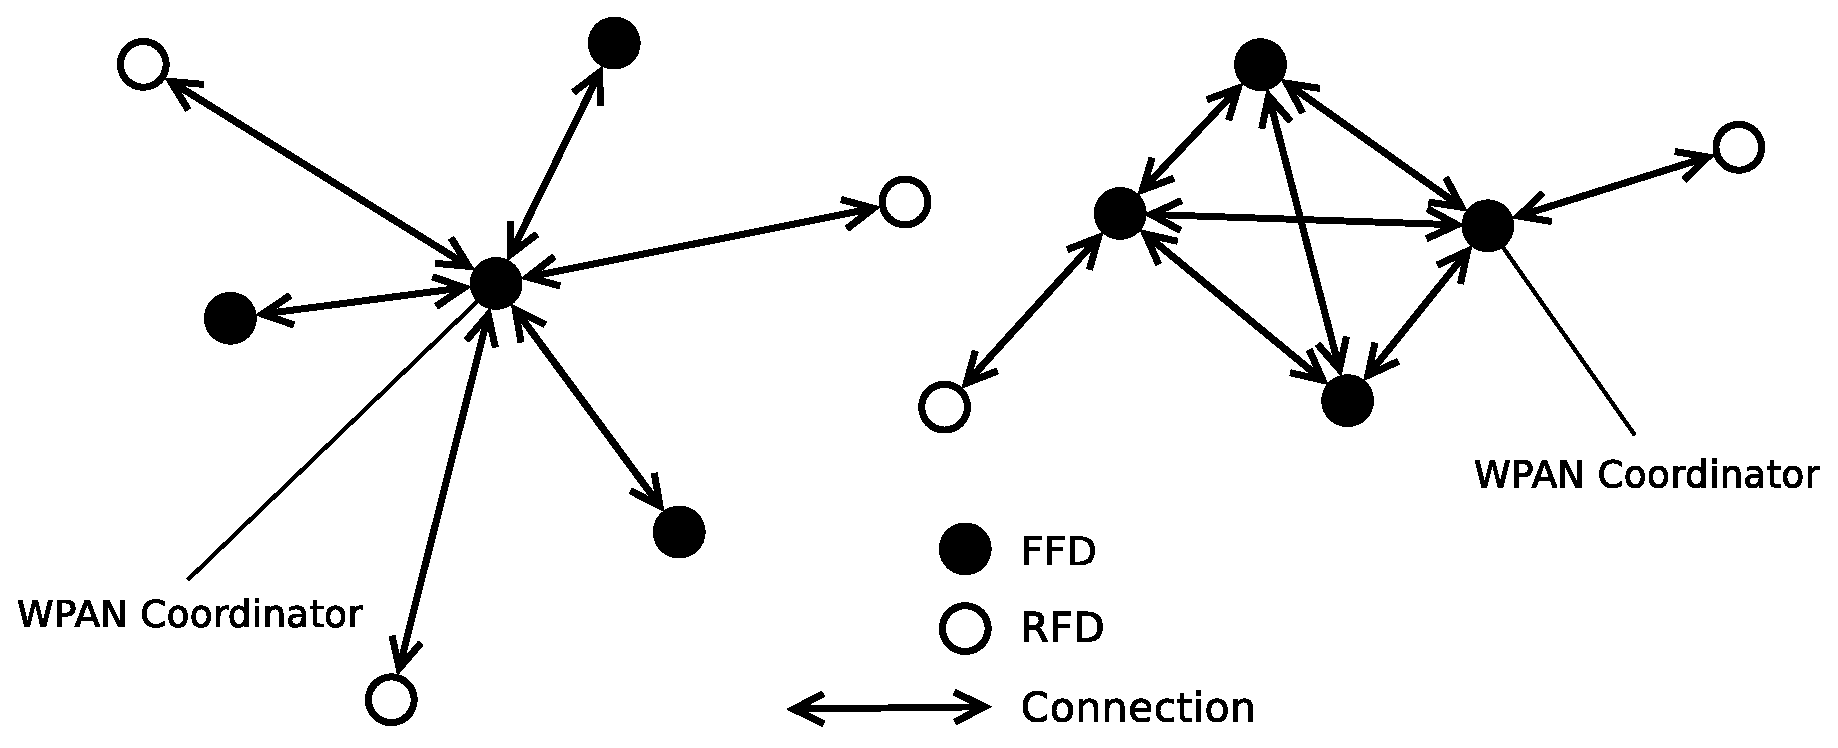
\includegraphics[width=0.9\textwidth]{WPAN_Network_Topologies.eps}
 \end{center}
 \caption{Star and peer-to-peer topology examples \cite{IEEE802.15.4-2003}}
 \label{fig:WPAN_Network_Topologies}
\end{figure}
\end{itemize}
This work will use the peer-to-peer topology as it is more flexible and scalable than the star topology. This topology is also
complexer, that is why a simpler case of peer-to-peer topology is selected, the tree topology. In this case all devices are
structured hierarchically and all of them have a father with whom they communicate, excepting the \ac{WPAN} Coordinator who is on the top of the network.

For this topology, a Network Layer (not provided in 802.15.4) is needed. For routing purposes only the short address (16 bits),
from the 2 kind already commented, will be used. This is to make packets as short as possible.

\section{Physic Layer}

Although for this work \ac{PHY} Layer has not as much importance as the \ac{MAC} Layer, there are some aspects that are important and 
that are good to know. This section will focus just on this aspects.

Some of the tasks developed by the \ac{PHY} Layer are:

\begin{itemize}
 \item \textbf{Switches on and off the radio transceiver.} Transceiver has 3 operation modes, \ac{Tx}, \ac{Rx} and sleeping, \ac{PHY}
layer must commute among this modes by \ac{MAC} layer petition. The standard defines that the change time between \ac{Rx} and 
\ac{Tx} and vice versa cannot be bigger as 12 symbols (\textit{aTurnaroundTime} = 12 symbols = 192 $\mu$s for 2.4 GHz).
 \item \textbf{Performs the \ac{ED} of the channel.} \ac{PHY} layer measures the power level of the channels to choose the best one
to transmit, this measurement lasts exactly 8 symbols.
 \item \textbf{Performs \ac{CCA} to check the channel.} This indicator is a part of \ac{CSMA/CA} algorithm as it will be seen later. The
\ac{CCA} is requested by the \ac{MAC} Layer and the \ac{PHY} Layer returns IDLE or BUSY depending on the channel situation. This \ac{CCA}
period lasts exactly like the \ac{ED}, 8 symbols (128 $\mu$s at 2.4 GHz).
 \item \textbf{Channel frequency selection.} As it was already commented, the 802.15.4 standard contemplates 3 different frequency 
ranges, although this possibility, only the 2450 MHz will be used in this work. At this frequency, the standard stipulates 
the use of a \ac{O-QPSK} modulation with a symbol rate of 62,5 symbol/s. As this modulation makes 4 bit per symbol, we get 
a 250 bit/s bit rate. This frequency range, has 16 different channels with a 5 MHz separation between them, the number of 
this channels goes from 11 to 26.
 \item \textbf{Data transmission and reception.} According to the standard, the \ac{PHY} Layer must be able to transmit with a minimum
power of 1 mW and it must have a sensibility of at least -85 dBm. Figure \ref{fig:PPDU} shows the physical level frame structure.

\vspace*{1cm}

\begin{figure}[here]
 \begin{center}
  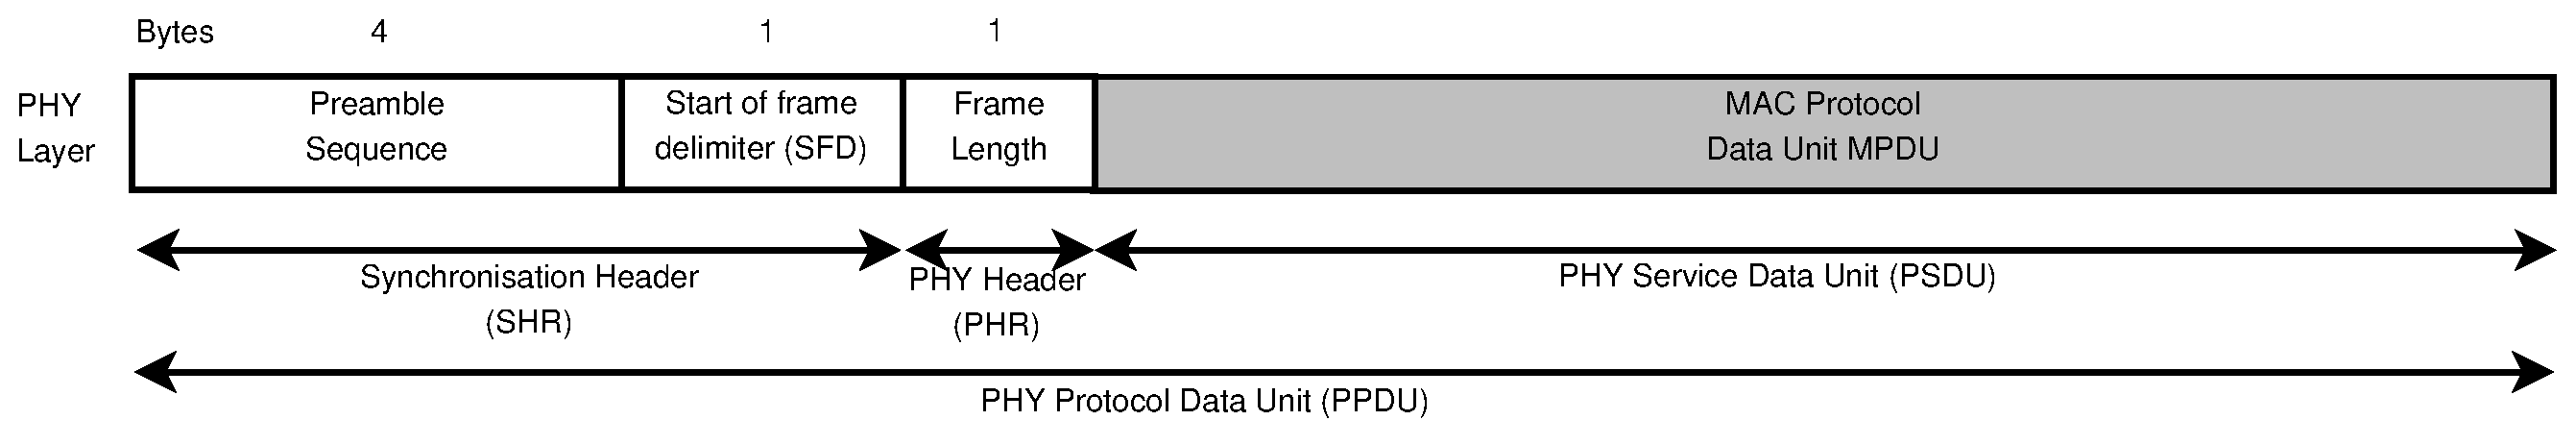
\includegraphics[width=0.9\textwidth]{PPDU.eps}
 \end{center}
 \caption{\ac{PHY} Layer frame \cite{IEEE802.15.4-2003}}
 \label{fig:PPDU}
\end{figure}
\end{itemize}



\section{\ac{MAC} Layer}

Non-Beacon mode as is more flexible for our purposes, but we have to sleep the node manually from the App layer


\clearpage{\pagestyle{empty}\cleardoublepage}
\chapter{Protocol Design}
\label{chap:protocoldesign}

In the state of the art, there are different protocols constructed over \ac{IEEE} 802.15.4, probably the most popular is ZigBee \cite{Zigbee}. 
Some of these protocols are prepared for low consumption, but, looking for it, it was found that none of them is really focused on localization. 
To cover this necessity, as an alternative, \ac{LPL} and \ac{OLP} \cite{LPLandOLP} protocols were proposed in the department. These protocols 
are based on \ac{IEEE} 802.15.4 and are specifically designed for low consumption localization. In the next sections a brief overview will be 
given, for a deeper view, please consult \cite{LPLandOLP}.

\section{\ac{LPL} and \ac{OLP}}

\ac{LPL} and \ac{OLP} \cite{LPLandOLP}, are two protocols designed for localization, in particular localization using \ac{RSSI} 
values. These values give an idea of the received signal strength in the device, knowing that the higher this value,
the nearer the device. \ac{RSSI} have the big advantage that its value is already included in all packets a device receives. There
is therefore no need for special hardware or data to be prepared or obtained like in other methods (Ultra Wide Band e.g.). But \ac{RSSI} 
values have a big problem for localization, its dispersion is very big, making the localization resolution (in some cases up to 
many meters \cite{fingerprint}) inappropriate for some applications. 

However, this resolution problem can be solved. One solution is using localization techniques like ``fingerprint 
technique'' \cite{fingerprint} to improve the resolution. Another option is, taking more than one \ac{RSSI} value to obtain a more stable 
result. This technique has one big challenge, the more values are taken, the higher the energy consumption. Without a good approach, 
the \ac{MN} would need to listen to the channel most of the time waiting to receive packets from \ac{AN} to obtain \ac{RSSI} values. 
This way a lot of energy would be wasted just doing nothing during what is called idle listening. \ac{LPL} and \ac{OLP} propose two different 
approaches to solve this.

Another important aspect in localization is which kind of node calculates the position. Three different alternatives can be obtained.

\begin{itemize}
 \item \textbf{Centralized.} A central computer receives the \ac{RSSI} values from all \acp{AN} in the network and calculates the positions of 
the \acp{MN}. The advantage is that the computer can use complicate algorithms to obtain better results, but this method 
charges the network with a lot of traffic, specially if the \ac{MN} needs to know its position after calculation.
 \item \textbf{Distributed-A.} The \ac{AN} gets the \ac{RSSI} values directly from the packet sent by the \ac{MN}, and this \ac{AN}
calculates directly the \ac{MN} position. This method does not charge the network like the centralized approach but the resolution 
is not that good. It is important to note that each \ac{MN} has a ``selected \ac{AN}''. This \ac{AN} is the one in charge to 
calculate \ac{MN} position and the one the \ac{MN} communicates with and through. This \ac{AN} is usually the closest one to 
the \ac{MN}.
 \item \textbf{Distributed-M.} In this mode, the \ac{MN} is who calculates directly its position from \ac{RSSI} values obtained from \acp{AN}.
The problem is that \acp{MN} cannot use powerful localization algorithms. This solution almost does not charge the network.
\end{itemize}

The protocols \ac{LPL} and \ac{OLP} are going to use different phases for different behaviors, and these phases will be repeated cyclically. To 
make this possible, all nodes have to start the phases at the same time. This makes necessary a good synchronization among all nodes.
Nodes will get the synchronization information from their parents (do not forget that a tree topology is used) using an active or a passive synchronization. 
To get a graphical explanation check Figure \ref{fig:synchronization}.

\begin{itemize}
 \item \textbf{Passive Synchronization.} The parent starts the process sending a packet (R1) to \ac{MAC} Layer to be transmitted, this packet is
created at the time-stamp Tx1, and includes this time, the time until the next phase start (TF) and info about this phase. Due to random time in 
\ac{CSMA/CA} process and other processing times, R1 is not transmitted immediately but in Tx2. When the packet is transmitted, \ac{MAC} Layer informs
the application layer and this creates another packet (R2) including the new time-stamp Tx2. At the child, 2 packets will be received, R1 and 
R2 in times Rx1 and Rx2 respectively. Calculation of next phase start, from the child's point of view (TZ), is accomplished like in (\ref{mat:pasivesync}).

\begin{equation}
  TZ = TF - (Rx2 - Rx1) - (Tx2 - Tx1)
  \label{mat:pasivesync}
\end{equation}

\begin{figure}[ht]
 \begin{center}
  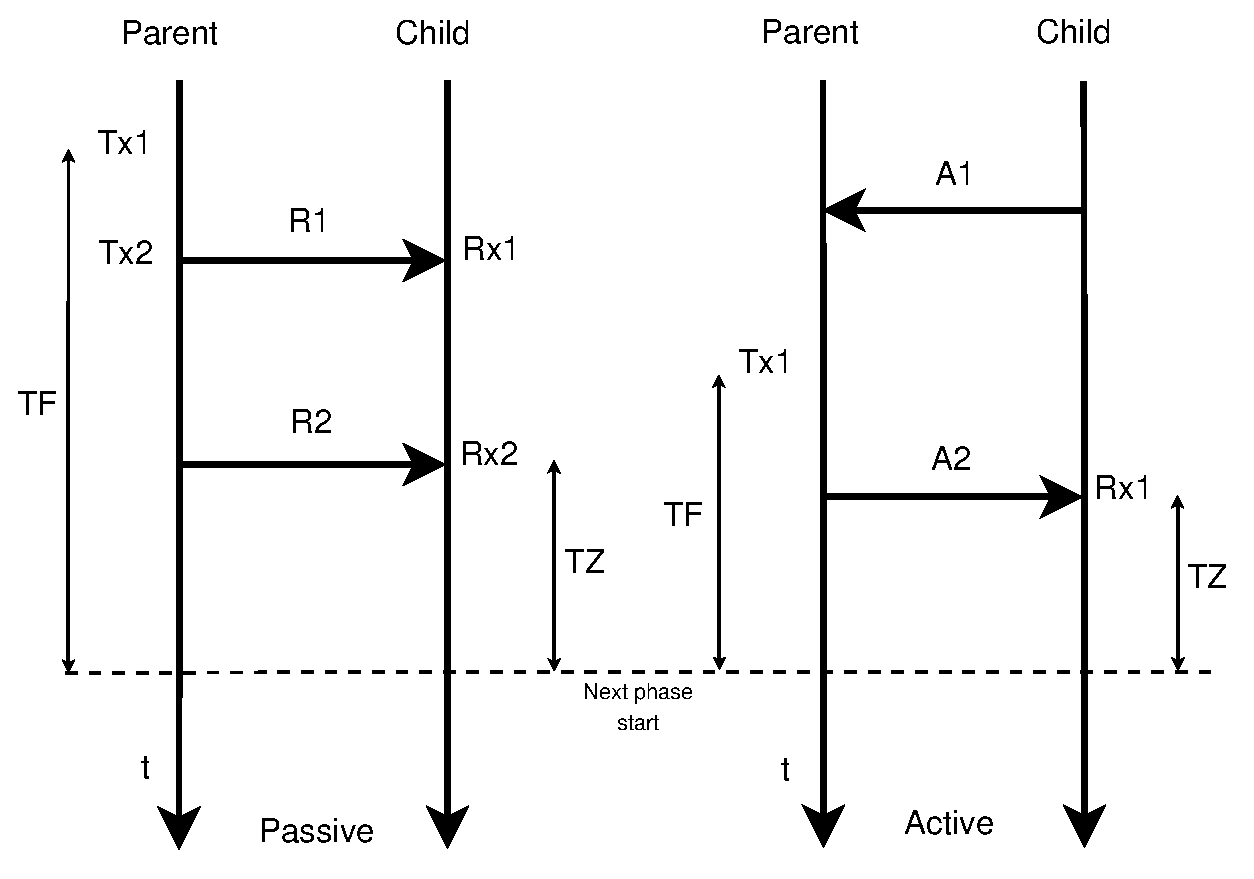
\includegraphics[width=0.6\textwidth]{synchronization.eps}
 \end{center}
 \caption{Passive and Active Synchronization \cite{LPLandOLP}}
 \label{fig:synchronization}
\end{figure}
 
 \item \textbf{Active Synchronization.} In the active synchronization, the child starts the process sending a synchronization request (A1).
Then the parent answers with packet A2, which contains the time until the start of the next phase (TF). The child can calculate this time
with the equation in (\ref{mat:activesync}).

\begin{equation}
  TZ = TF - C
 \label{mat:activesync}
\end{equation}

The C parameter in (\ref{mat:activesync}), represents an estimation of all the processing times and random times from \ac{CSMA/CA}. For that reason 
this method is not so exact like the passive one, but it does not need two packets.
\end{itemize}

In the following subsections, both protocols \ac{LPL} and \ac {OLP} are going to be explained.

\subsection{\acl{LPL}}

To reduce the idle listening, and therefore the energy consumption, this protocol proposes that \acp{MN} do not listen to the \acp{AN}. Instead, the
\acp{MN} are the ones who transmit and the \acp{AN} the ones who listen and transmit this information to the central computer. This protocol is 
divided into three phases which can be appreciated in Figure \ref{fig:LPL}.

\begin{figure}[ht]
 \begin{center}
  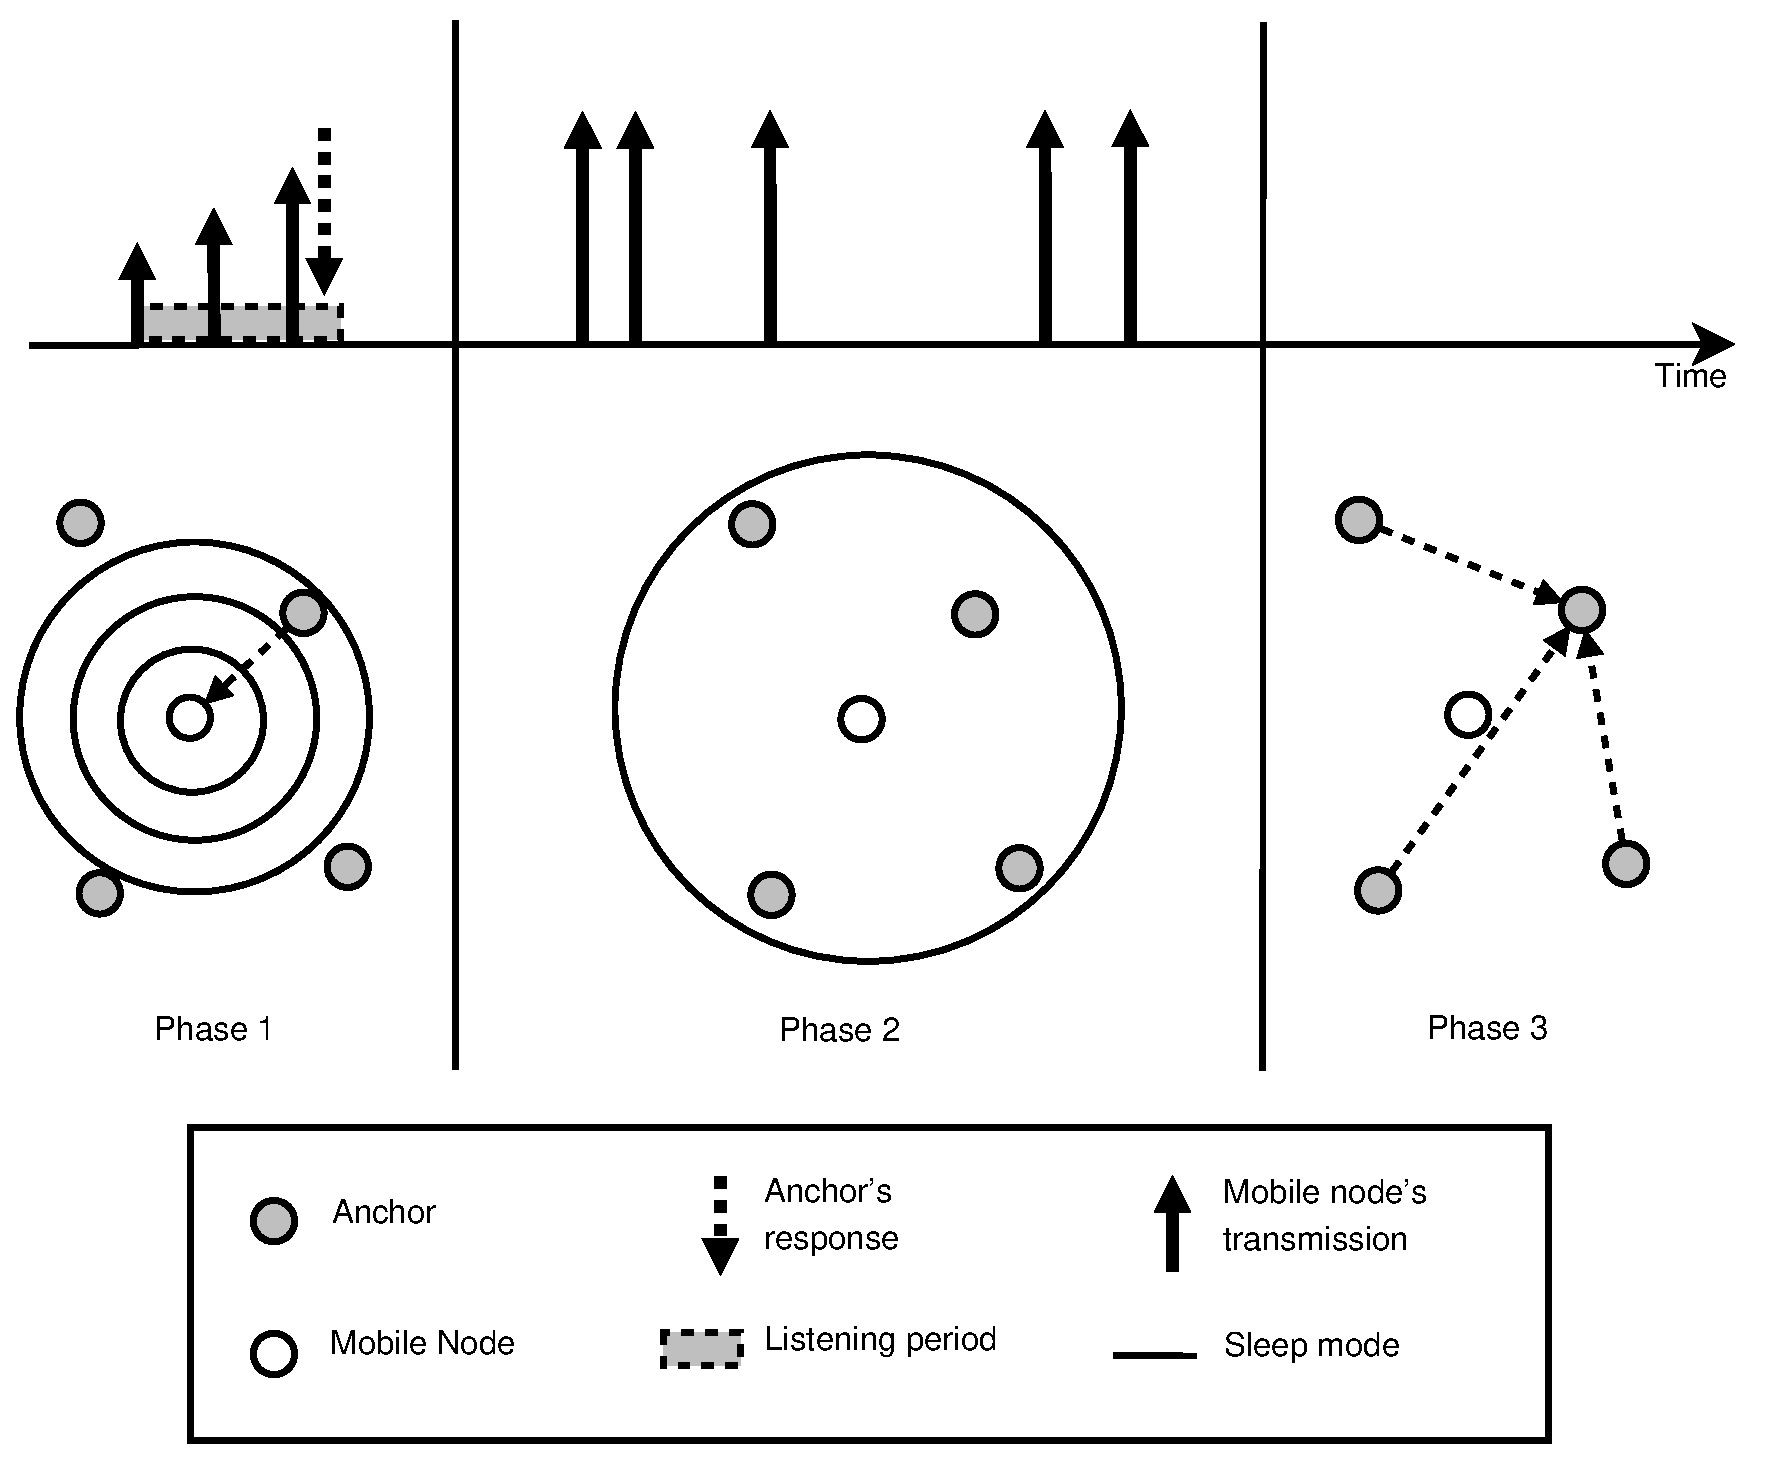
\includegraphics[width=0.7\textwidth]{LPL.eps}
 \end{center}
 \caption{LPL Phases \cite{LPLandOLP}}
 \label{fig:LPL}
\end{figure}

\begin{itemize}
 \item \textbf{Phase 1:} In this phase, \ac{MN} selects a random time to broadcast a synchronization request, starting with the minimum power,
and increasing this power until it receives an answer from an \ac{AN}. This will be the selected \ac{AN}, and the answer will contain information
about the phase times. This process makes sure that only the nearest \acp{AN} answer to the synchronization request. In the next phase 1, if 
the \ac{MN} needs to know its position, it asks its selected \ac{AN} about this information, and if not, it just synchronizes.
 \item \textbf{Phase 2:} In phase 2, the \ac{MN} broadcasts several packets in random times to minimize the collisions. Each time the node is not
transmitting, it goes to sleep. This way \acp{MN} are awake only when they transmit, eliminating the idle listening. The \acp{AN} that
received these broadcasts, store the read \ac{RSSI} values and the selected \ac{AN} address.
 \item \textbf{Phase 3:} During this phase, the \acp{MN} sleep and the \acp{AN} send the measured \ac{RSSI} values to the selected \ac{AN}. 
This \ac{AN} will calculate the \ac{MN} position in Distributed-A case or send the data to a central computer in Centralized case. In this phase, both 
synchronization among the \acp{AN} and the network configuration take place.

This protocol, has some disadvantages that make it not suitable for all conditions:

\begin{itemize}
 \item Hidden Terminal Problem. This is a serious problem not only because it could cause big idle listening in phase 2, but also because the number
of collisions could be high and the packets would have been sent for nothing, wasting a lot of energy. In phase 1, it could also 
happen that, if two \acp{MN} transmit at the same time, the selected \ac{AN} might not be the closest one to the \ac{MN} but one with a bad connection.
 \item High \ac{MN} number. If the number of \acp{MN} is high, phase 2 is going to be full of collisions and therefore, the idle listening will be
high. This problem would be worse due to the hidden terminal problem.
 \item Selected \ac{AN} selection. In phase 1, if many \acp{AN} are close to the \ac{MN}, all of them are going to try to answer causing collisions. Also, 
when the \acp{AN} are not close to the \ac{MN}, a lot of energy is wasted in the \ac{MN} trying to detect gradually the selected \ac{AN}.
\end{itemize}


\end{itemize}


\subsection{\acl{OLP}}

In the case of \ac{OLP} protocol and unlike \ac{LPL}, the \ac{MN} is the one who listens. This protocol is also divided in 3 phases, 2 of 
them can be appreciated in Figure \ref{fig:OLP}.

\begin{figure}[ht]
 \begin{center}
  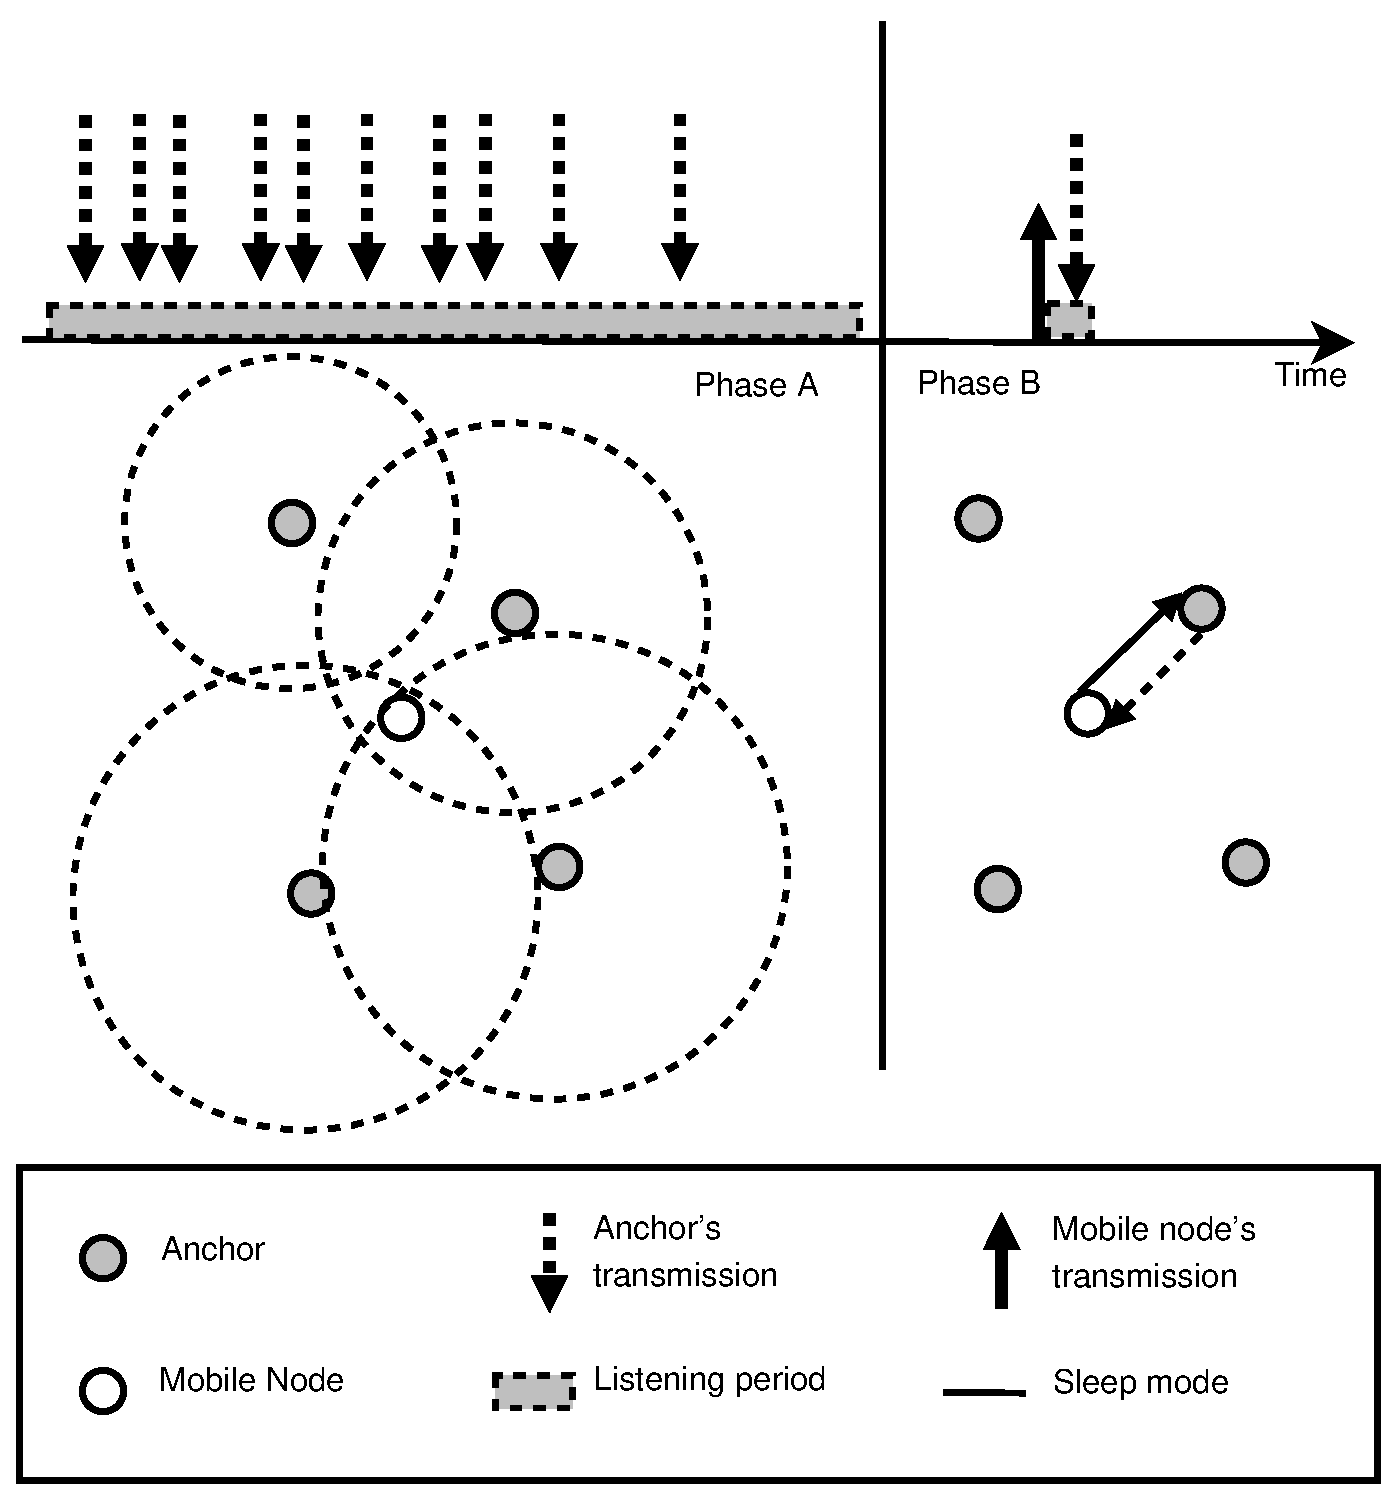
\includegraphics[width=0.55\textwidth]{OLP.eps}
 \end{center}
 \caption{OLP Phases \cite{LPLandOLP}}
 \label{fig:OLP}
\end{figure}

\begin{itemize}
 \item \textbf{Phase A:} In this phase, the \acp{AN} transmit their broadcast packets. Thanks to the synchronization among \acp{AN}, the inter-arrival 
time is reduced, decreasing so the idle listening. These packets also contains synchronization information for the \ac{MN}. In this phase \ac{RSSI} values are received and stored
by the \ac{MN}. Then it goes to sleep.
 \item \textbf{Phase B:} In this phase and in Distributed-M mode, the \ac{MN} will use easy localization algorithms together with all the obtained
\ac{RSSI} values to calculate its position. In case of Distributed-A or Centralized mode, the \ac{MN} will send a report to the selected \ac{AN}, taken 
from the highest \ac{RSSI} value, with all the stored \ac{RSSI} values in Phase A. The selected \ac{AN} will answer with an \ac{ACK}. In the following
phase B, the \ac{MN} will ask the selected \ac{AN} about its position in case it needs it.
 \item \textbf{Phase C:} Like in \ac{LPL} this Phase is reserved for communication among \acp{AN} and network configuration.
\end{itemize}

\ac{OLP} has also some problems:

\begin{itemize}
 \item Synchronization. In this protocol, a really good \acp{AN} synchronization is needed to make the idle listening in phase 1 from the 
\acp{MN} as low as possible. This is not easy, specially with a tree structure where the synchronization error will be increased and 
propagated through the tree.
 \item \ac{MN} listens too much. The \ac{MN} is listening during long periods of time where all the \acp{AN} are transmitting, some times it
could even happen that the \ac{MN} it is not at a reachable distance from the \ac{AN} that is transmitting, listening in this moment just 
for nothing.
 \item Hidden Terminal Problem. If the \acp{AN} are not good synchronized to avoid this problem, the \acp{MN} would get many invalid 
packets, what means a waste of energy. If the number of \acp{MN} is big, then in phase 2 we could have many collision problems.
 \item Temporal \ac{RSSI} Correlation. As the \ac{RSSI} values are very correlated in near times \cite{RSSIcorrelated}, receiving all 
the packets so close in time would not contribute to have a better and more stable \ac{RSSI} measurement.
\end{itemize}
 

\section{High Configurable Protocol proposal}
\label{sec:ProtocolDescription}

From the previous section and according to the results in \cite{LPLandOLP}:
\begin{quote}
``LPL consumes lower energy than OLP when many RSSI samples are required from many ANs. On the other hand,
OLP becomes more energy efficient than LPL when there are several MNs and few RSSI samples are needed.''\cite{LPLandOLP}
\end{quote}

From this could be extracted that depending on the application and the network load, it could be better that some nodes could have a 
configuration where their main action is listening and others could have a configuration where their main action is broadcasting. This 
configuration should be variable depending on the current network situation and the necessities of the node. From this arises the necessity
of a High Configurable Protocol with different node configurations.

As it was seen, \ac{OLP} and \ac{LPL} localization protocols, are based on \ac{RSSI} values. This work is also based on localization using 
\ac{RSSI} values. Anyhow, this simulation work proposes a framework for the protocol and does not try to locate any node, it concentrates
in the communication aspects and defines a base for the protocol to be developed further in future works.


\subsection{Node Configurations}

From the Table \ref{tab:wsn_applications} (page~\pageref{tab:wsn_applications}) where different applications for \ac{WSN} where stated and the
previous quotation, it is possible to extract these four different node configurations.

\begin{itemize}
 \item \textbf{Mode 1.} This is the normal configuration, when the \ac{MN} does not have any special need. A \ac{MN} with this configuration,
will listen to the \acp{AN} and then send the selected \ac{AN} a packet with the measurements. This is equivalent to having just \ac{OLP}. This
configuration supports the Centralized and Distributed-A working modes.

 \item \textbf{Mode 2.} This configuration mode is similar to mode 1, but in this case it is prepared to work only with Distributed-M working mode.
From time to time, if it is needed, the \ac{MN} could send the estimated positions to its selected \ac{AN}.

 \item \textbf{Mode 3.} This configuration, also called \ac{VIP} mode, is used when the node's battery is in a critical situation.
This configuration is similar to \ac{LPL} where the \ac{MN} broadcasts and the \acp{AN} receive the packets and send them to a coordinator that
will be able to estimate \ac{MN} position. When it is needed, a way for the \ac{MN} to request its position is provided, this will be explained 
later. The number of sent broadcasts is defined with the parameter \textit{NumberOfBroadcasts}.

 \item \textbf{Mode 4.} Unlike the previous configuration, this configuration is for nodes without battery problems, and with a high accuracy
need. This configuration is a mix of Modes 1 and 3, the \ac{MN} listens to the \ac{AN}'s broadcasts but also they broadcast their
own packets to be measured by the \acp{AN}. All this information is sent together to a coordinator that will estimate the \ac{MN} position.
This Mode as well as Mode 3 loads the network so much and will be used just when strictly needed. The number of sent broadcasts is also defined with 
the parameter \textit{NumberOfBroadcasts}.
\end{itemize}

This is just a brief description of the different configurations. As the protocol is yet to be explained, a full behavior description from 
every configuration will be done later together with the protocol description.

\subsection{Protocol Description}

From the previous section, it is obtained that this protocol, needs at least three different phases to work. One of the phases is a Sync 
Phase, where the \acp{AN} will transmit broadcasts and the \acp{MN} will listen to get \ac{RSSI} values and synchronize. Another needed 
phase is a phase where \acp{AN} and \acp{MN} could communicate among them. And the last required phase, is the one where the \acp{AN} could 
communicate with each other to and from the coordinator.

\acp{MN} configured in Mode 3 are nodes with critical battery. These nodes must not waste energy, and this means their idle listening must be
as low as possible. As these nodes will not waste time listening and will just transmit broadcasts, it could be interesting reserving a phase
just for them, where their transmissions will not interfere with the ones from the rest of the \acp{MN}. This phase will be called \ac{VIP} 
Phase. It is clear, that the number of \ac{VIP} \acp{MN} cannot be too big, if so, their exclusivity will not be anymore exclusive.
This phase should not last too long, as there are still many other \acp{MN} to transmit and the phases collection would become too long.
The phase for communication among \acp{MN} and \acp{AN} will be named Report Phase, and here is where Mode 4 \acp{MN} can make 
their broadcasts and where communication among \acp{MN} and \acp{AN} can take place.

The main purpose of the phase where \acp{AN} communicate with each other, is to transmit information between the coordinator, also called sink, and 
the \acp{MN}. That is the reason why this phase will be called ComSink Phase. This phase should be the biggest one, as all traffic from 
the \acp{MN} should reach the sink and come back, and all \acp{AN} must transmit their own \acp{MN} information and route the one coming from
their sons or father. As the traffic in this phase will be high, it could be useful to separate up-links traffic and down-links traffic. 
ComSink Phase will be divided in ComSink Phase 1 (up-links) and ComSink Phase 2 (down-links).

As it was said, \ac{RSSI} values are very correlated in time instants that are next to each other \cite{RSSIcorrelated}. That is why it could 
be favorable to distribute the Sync Phase to get better \ac{RSSI} samples. The whole period is formed by Sync Phase, Report Phase, \ac{VIP}
Phase, ComSink Phase 1 and ComSink Phase 2. If Report Phase and \ac{VIP} Phase are considered together in the phases distribution, Sync 
Phase can be divided into three phases separated in time: Sync Phase 1, Sync Phase 2 and Sync Phase 3. These sync phases will be intercalated 
between the other phases.

This phase collection will be repeated in time, being the period every phases collection repe\-ti\-tion. For a better understanding of this 
phase division, check Figure \ref{fig:ProtocolPhases}. This Figure will be explained in detail later.

\begin{figure}[ht]
 \begin{center}
  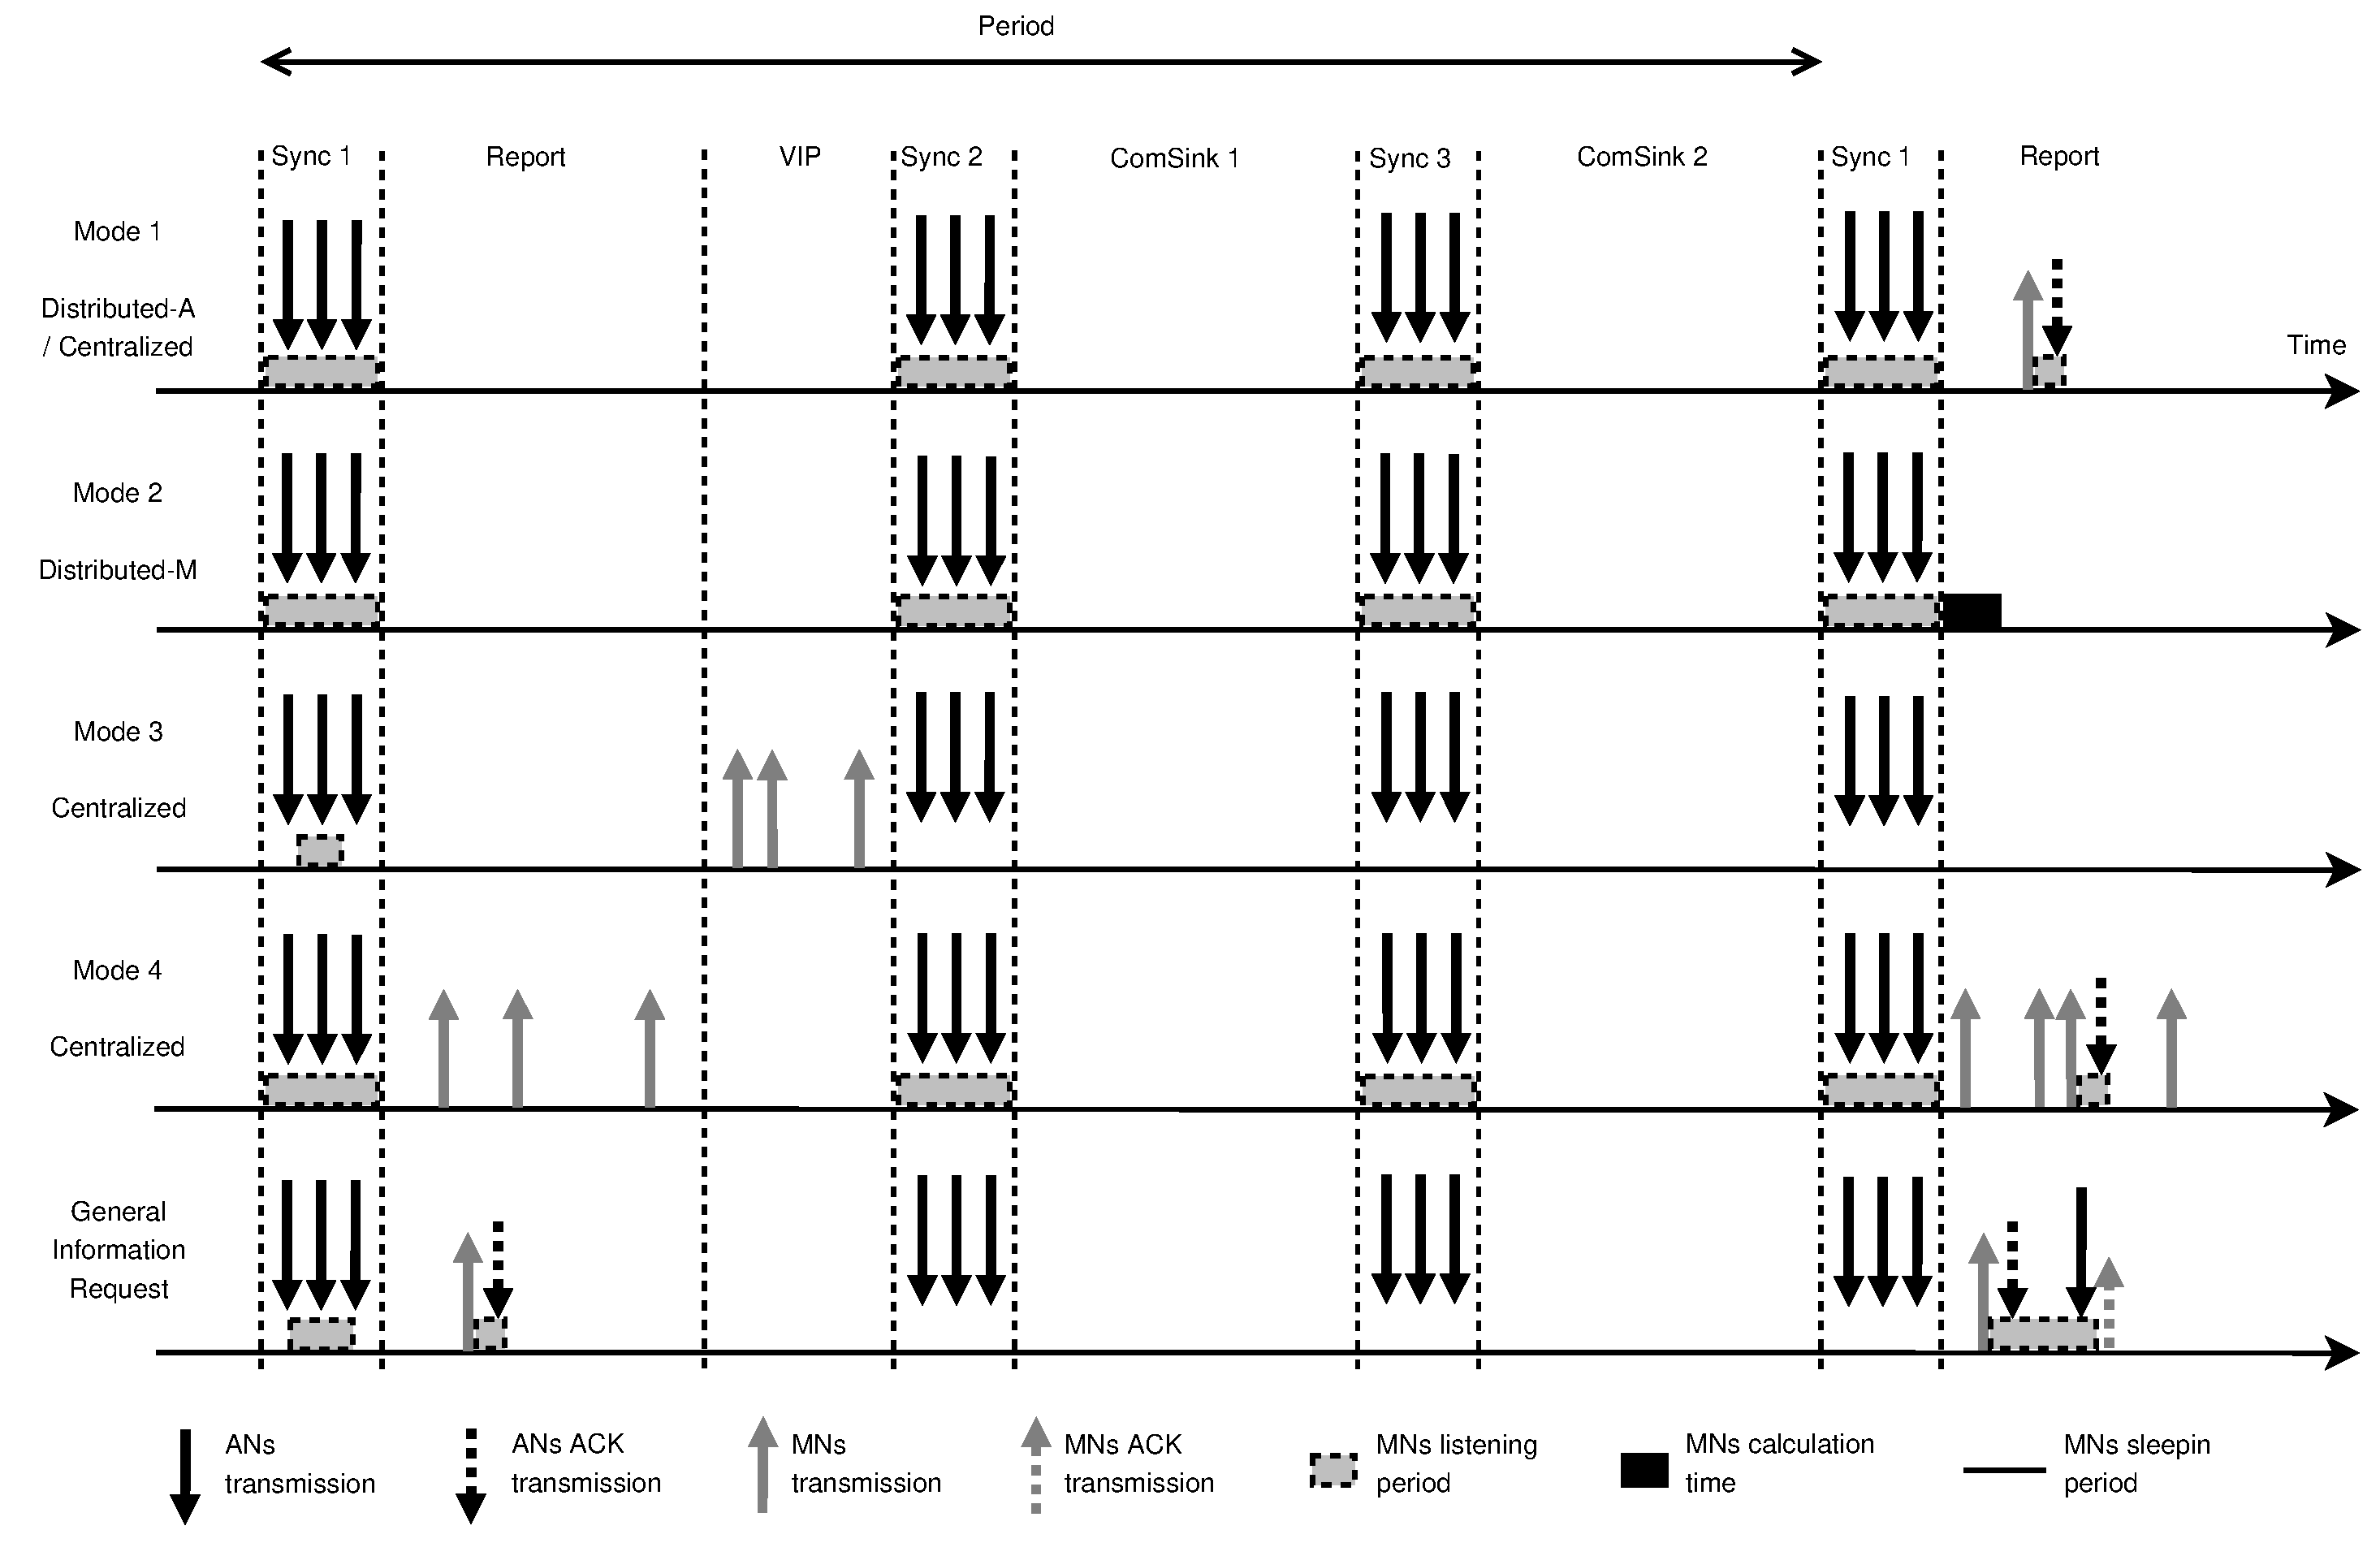
\includegraphics[width=1\textwidth]{ProtocolPhases.eps}
 \end{center}
 \caption{High Configurable Protocol Phases \cite{mipaper}}
 \label{fig:ProtocolPhases}
\end{figure}

The Figure \ref{fig:ProtocolPhases} is divided into 5 sections, one per Configuration Mode and the last one for explaining the General Information
Request. To understand properly how the protocol works, these sections have to be explained in detail:

\begin{itemize}
 \item \textbf{Mode 1.} \acp{MN} listen during the Sync Phases to the \acp{AN} broadcasts, and read the \ac{RSSI} values and send them
to their selected \ac{AN} during the Report Phase. This is obtained from the highest measured \ac{RSSI}. The selected \ac{AN} answers with an \ac{ACK} 
to the \ac{MN}. \acp{MN} sleep during the \ac{VIP}, ComSink 1 and ComSink 2 Phases as well as during Report Phase when no transmitting. 
\acp{AN} will communicate among them during ComSink 1 phase (up-links) and during ComSink 2 phase (down-links). This aspect is common for all the 
modes, that is why it will be commented only in this one. Whenever the \ac{MN} must communicate something to the selected \ac{AN} and no report 
is going to be sent during the period, it can schedule an extra report during the Report Phase. This extra report behavior is the same as the report 
where the \ac{RSSI} values are sent.
 
 \item \textbf{Mode 2.} Like in Mode 1, \acp{MN} listen during the Sync Phases to the \acp{AN} broadcasts, and read the \ac{RSSI} values. Instead
of sending them and due to the fact that packets also contain information of \acp{AN} localization, it is the \ac{MN} who calculates its own position 
and saves it. From time to time, this positions information will be sent to the coordinator via the selected \ac{AN} during the Report Phase. The 
selected \ac{AN} will answer with an \ac{ACK} to the \ac{MN} which will go to sleep. \ac{MN} sleeps, like Mode 1, during \ac{VIP}, ComSink 1 and ComSink 2 
Phases as well as during Report Phase when no transmitting.

 \item \textbf{Mode 3.} Unlike Mode 1 and 2, Mode 3 does not listen during the Sync Phases but sleeps. Once in a while, Mode 3 will not sleep during a 
Sync Phase and will listen just for a couple of packets (not the whole phase) to resynchronize. During the \ac{VIP} Phase, the \ac{MN} will broadcast
some packets that will be listened by the \acp{AN} in the surrounding. These \acp{AN} will send the \ac{RSSI} information to the coordinator during the 
ComSink 1 phase, and this will calculate the \ac{MN} position. As Mode 1, \acp{MN} in Mode 3 could schedule an extra report during Report Phase to
communicate something to the selected \ac{AN}. Mode 3 \acp{MN} sleep during Sync, Report, ComSink 1 and ComSink 2 phases as well as during \ac{VIP} phase
when not transmitting. Whenever a \ac{MN} sends an extra report, during that period it will not send the broadcasts during \ac{VIP} Phase, this is to 
save energy, as with the extra report it will send already \ac{RSSI} information to the selected \ac{AN}.

 \item \textbf{Mode 4.} This is a combination of Modes 1 and 3. On one hand, the \acp{MN} listen during Sync Phases to get \ac{RSSI} values and send them
to their selected \ac{AN} during Report Phase waiting for an \ac{ACK}. But on the other hand, they broadcast also their own packets during the Report Phase.
This broadcasted \ac{RSSI} values are sent by all \acp{AN} to the coordinator who with all these values and the values reported by the \ac{MN} through the 
selected \ac{AN}, calculates the \ac{MN} position. As for Mode 1, whenever a \ac{MN} wants to send something, it can schedule an extra report. This node sleeps
during \ac{VIP}, ComSink 1 and ComSink 2 phases as well as during Report Phase when no transmitting.

 \item \textbf{General Information Request.} What happens if a \ac{MN} wants to know its position? or if it wants to change its configuration, how does it
warn the coordinator? Thanks to the General Information Request, this can be solved. During Report Phase and using a report or extra report, the \ac{MN}
will activate in this packet an ASK flag to notify the selected \ac{AN} that some data (the requested info is given in this packet) will be requested 
during next period in Report Phase, then the \ac{AN} acknowledges the packet like always. During the next Report Phase, the \ac{MN} will generate an extra
report in case there is no scheduled one and will activate the Request flag to notify the \ac{AN} that it wants the data asked the previous period about. As soon
as the \ac{MN} receives the \ac{ACK} from the selected \ac{AN}, a timer starts. If during this timer no packet from the selected \ac{AN} is received, the whole
process is canceled and it could be tried again later. If during this timer the \ac{MN} receives a packet from the selected \ac{AN}, the \ac{MN} sends an
\ac{ACK} to the \ac{AN} and the process is finished. The \ac{AN} will send a packet to the \ac{MN} even to indicate that it has no information available.
Doing so, idle listening in \ac{MN} is avoided.

This process must be done from time to time even if the node does not have any change or requirement, because if the coordinator wants to communicate with a
\ac{MN}, which would be sleeping all the time, this is the only way to reach it.
\end{itemize}

Like in \ac{LPL}, all packets sent (report and broadcasts), are sent in a random time using \ac{CSMA/CA} to minimize collisions.

Previously, it was just defined the standard behavior of the different configurations, but to really extract a high configuration of the protocol, some 
parameters must be taken into account.

\begin{itemize}
 \item \textbf{activePhases -} These are the periods where the \acp{MN} are active with their standard behavior (the already commented in the previous page).
 \item \textbf{inactivePhases -} These are the periods where the \acp{MN} are sleeping during all the phases.
 \item \textbf{offsetPhases -} These are the periods to leave inactive before the first active period comes.
 \item \textbf{offsetSyncPhases -} This is the number of Sync Phases during the first active period where the \acp{MN} do not listen, it will be explained 
better with an example.
 \item \textbf{reportPhases -} One period out of \textit{reportPhases}, the \ac{MN} will send an extra report in case this period does not have already one
scheduled. This happens even if the period is an inactive one.
 \item \textbf{askFrequency -} Every \textit{askFrequency} number of extra reports, these will have the ASK flag activated.
 \item \textbf{offsetReportPhases -} These are the periods to leave before the first extra report is scheduled.
\end{itemize}
 
As an example to explain these parameters check Figure \ref{fig:parametersphases}, where the parameters take the following values: 

\begin{quote}
 \textit{activePhases} = 2 | \textit{inactivePhases} = 2 | \textit{offsetPhases} = 1 | \textit{offsetSyncPhases} = 1 | \textit{reportPhases} = 3 
| \textit{askFrequency} = 2 | \textit{offsetReportPhases} = 0
\end{quote}

In Figure \ref{fig:parametersphases} can be seen how the first period is left inactive due to the \textit{offsetPhases} = 1. Although the period
is inactive, it has an extra report (\textit{offsetReportPhases} is 0). As \textit{reportPhases} is 3, the first period of 3 will have an extra report (R1). 
Then, for two periods it will not be an extra report and then another extra report will be scheduled (R3). After the first inactive period, 2 active 
periods follow (\textit{activePhases} = 2). Then 2 inactive periods (\textit{inactivePhases} = 2) and so on. From now on, this work will call ``report'' to the one 
corresponding to the standard behavior of \acp{MN} Mode 1 and 4, which is transmitted in every last active period. And ``extra report'' will be 
the one scheduled with \textit{reportPhases} frequency. Take into account that, while reports are sent just for Modes 1 and 4 and only in the last active period,
broadcasts in Modes 3 and 4 are send every active period. Note also that, if an extra report is scheduled in an inactive period, the \ac{MN} must
listen to the first Sync Phase of the period to get to know which is its selected \ac{AN}.

\begin{figure}[H]
 \begin{center}
  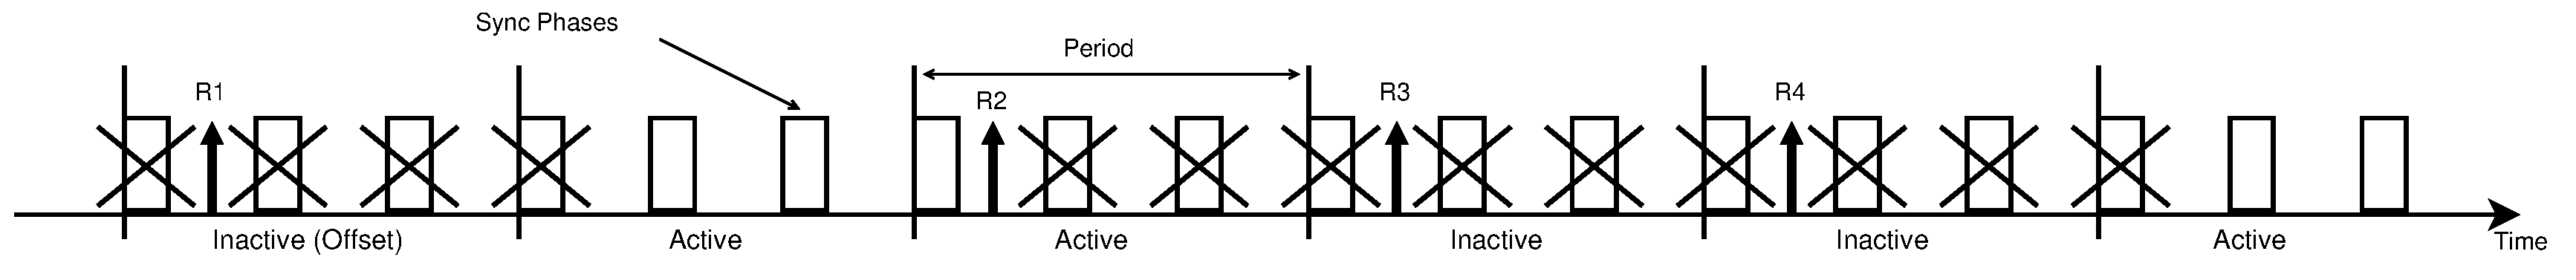
\includegraphics[width=1\textwidth]{parametersphases.eps}
 \end{center}
 \caption{Parameters Example}
 \label{fig:parametersphases}
\end{figure}

The last period in a group of active periods, is the one where the position is calculated (for mode 2) or the \ac{RSSI} values are sent (R2) to the selected 
\ac{AN} (for modes 1 and 4). After this moment, it makes no sense for the \acp{MN} to listen to more Sync Phases, that is why they are crossed out. 

It can also be seen that due to \textit{offsetSyncPhases} = 1, the \ac{MN} is not listening to the first Sync Phase from the first active period in the active
periods collection. Thanks to this, it is possible changing \textit{offsetSyncPhases} and \textit{activePhases}, to decide how many Sync Phases will the \ac{MN}
listen to before calculating its position or sending the measured \ac{RSSI} values to its selected \ac{AN}. In this case three Sync Phases were listened to.

Last but not least, as \textit{askFrequency} = 2, every 2 extra reports, the ASK flag will be activated, in this case in R3. This flag indicates the 
\ac{AN} that the \ac{MN} will ask for some information during the next period, this is made with R4. This request packet does not necessarily correspond
to a normal report (modes 1 or 4) or to an extra report, but if the period has already one of these reports, the same one will be used, activating a request
flag in it.


\section{Sync Phase detail}

To make possible that all nodes know when all phases within a period start, it is really important that all of them are correctly synchronized. This is 
possible thanks to the Sync Phase, and that is why this phase will be studied in detail. It has to be taken into account that all nodes know the duration
of the phases and the period.

The separation between Sync Phases allows the \ac{MN} to take \ac{RSSI} measurements at different time instants within the period. It increases the 
probability that the \ac{RSSI} values are not correlated. The minimal separation between Sync Phases can be defined by considering the coherence time 
of the signal.  According to \cite{RSSIcorrelated}, the attenuations of the signal at two time instants separated by more than the coherence time 
are weakly correlated. The coherence time depends on the carrier frequency and the speed of the \acp{MN}. In \cite{RSSIcorrelated2} a coherence time 
of 125 ms was calculated for a node operating at 2.4 GHz, when it moves at 1.2 Km/h.

In our network the coordinator is the time reference which initializes the synchronization propagation. The \acp{AN} start broadcasting packets only 
when they are synchronized. Between transmissions the \ac{AN} listens to the new synchronization packets from all surrounding \acp{AN}. In this way 
it is possible that the \acp{AN} are always synchronized.

Two scenarios are going to be described and studied, in the first scenario, the Sync Broadcasts, are going to be randomly distributed through the Sync 
Phase, in the second scenario, Sync Phase is going to be divided into slots where all \acp{AN} broadcasts will be distributed.

In both scenarios, the \acp{AN} broadcast packets contain information about the synchronization of the network as well as the position 
of the \acp{AN}. These packets are used by the \acp{MN} to obtain \ac{RSSI} measurements and to synchronize. This way they can know when the start time of 
the next phase will take place.

\subsection{Random Sync Phase}

In this first scenario, \ac{AN}'s application level, calculates the time to the next phase. This information is included in the synchronization packet 
and sent to the \ac{MAC} layer for its transmission. Due to the random time of the \ac{CSMA/CA} process, the packet is not immediately transmitted. This 
random delay degrades the synchronization performance, because it is unknown by the receivers. A possible solution to this problem is to transmit a 
second packet, which informs about the \ac{CSMA/CA} delay of the first transmission (passive synchronization, see Figure \ref{fig:synchronization}, 
page~\pageref{fig:synchronization}). The main disadvantage of this proposal is that the \ac{MN} needs to listen to at least two synchronization packets 
from the same \ac{AN} in order to be synchronized.

In order to reduce the idle listening period in the \acp{MN}, this work proposes to configure the \ac{AN}'s \ac{MAC} Layer to disable its random 
Backoff delay. Thus, it is possible to have a constant offset time between the moment when the remaining time was calculated and the moment of the 
transmission. According to the 802.15.4 Standard the Backoff delay can be disabled by setting the parameters \textit{macMaxCSMABackoffs}, 
\textit{macMinBE} and \textit{macMaxBE} to zero. Under this \ac{MAC} configuration, in case the channel is busy during the first \ac{CCA} detection, a \ac{CAF} 
is sent to the application level, which can try a retransmission. To avoid all \acp{AN} trying to transmit at the same time and therefore making easier 
the access to the channel, a random delay has to be generated in the application level before sending the packet. This way, the time until the start of the
next phase, will still be known in the application layer, but still random.

Hidden terminal problem has a high importance in this scenario, provoking collisions between Sync Packets. To prove this, during the Chapter 
\ref{chap:simulationandresults}: \nameref{chap:simulationandresults}, a scenario avoiding hidden terminal problem and another having it will be simulated.

\subsection{Slotted Sync Phase}
\label{subsec:slottedsyncphase}

To make the most of Sync Phase and avoid random times where \acp{MN} are listening without any benefit, a broadcast transmission distributed into slots is proposed.

A first approach is to divide the Sync Phase in as many slots as \acp{AN} in the network. This way each \ac{AN} could transmit a broadcast per Sync Phase.
But as it was already said, it is beneficial to be able to listen to more than one \ac{RSSI} value to get a more stable value due to its dispersion. This
way, the parameter \textit{syncPacketsPerSyncPhase} is presented. This parameter defines in how many parts Sync Phase will be divided (typically three). Each of 
these parts, will be divided in as many slots as \acp{AN} in the network. For example, if \textit{syncPacketsPerSyncPhase} = 3 and there are 9 \acp{AN} in the 
network, the Sync Phase will be divided into 27 slots. The problem is, that this way, Sync Phase could be very long when the number of \acp{AN} increases and therefore
\acp{MN} would be listening to the channel for too much time. Most of this time while \acp{AN} at not reachable distance transmit (idle listening).

A way to solve this, is to reuse the slots allowing that \acp{AN} far from each other could transmit at the same time. To avoid Hidden Terminal 
Problem, an \ac{AN} cannot transmit at the same time as its neighbors, or all the neighbors of them. With neighbors, is understood all \acp{AN} at a 
reachable distance. As an example check Figure \ref{fig:ejemplonetslots}.

\begin{figure}[ht]
 \begin{center}
  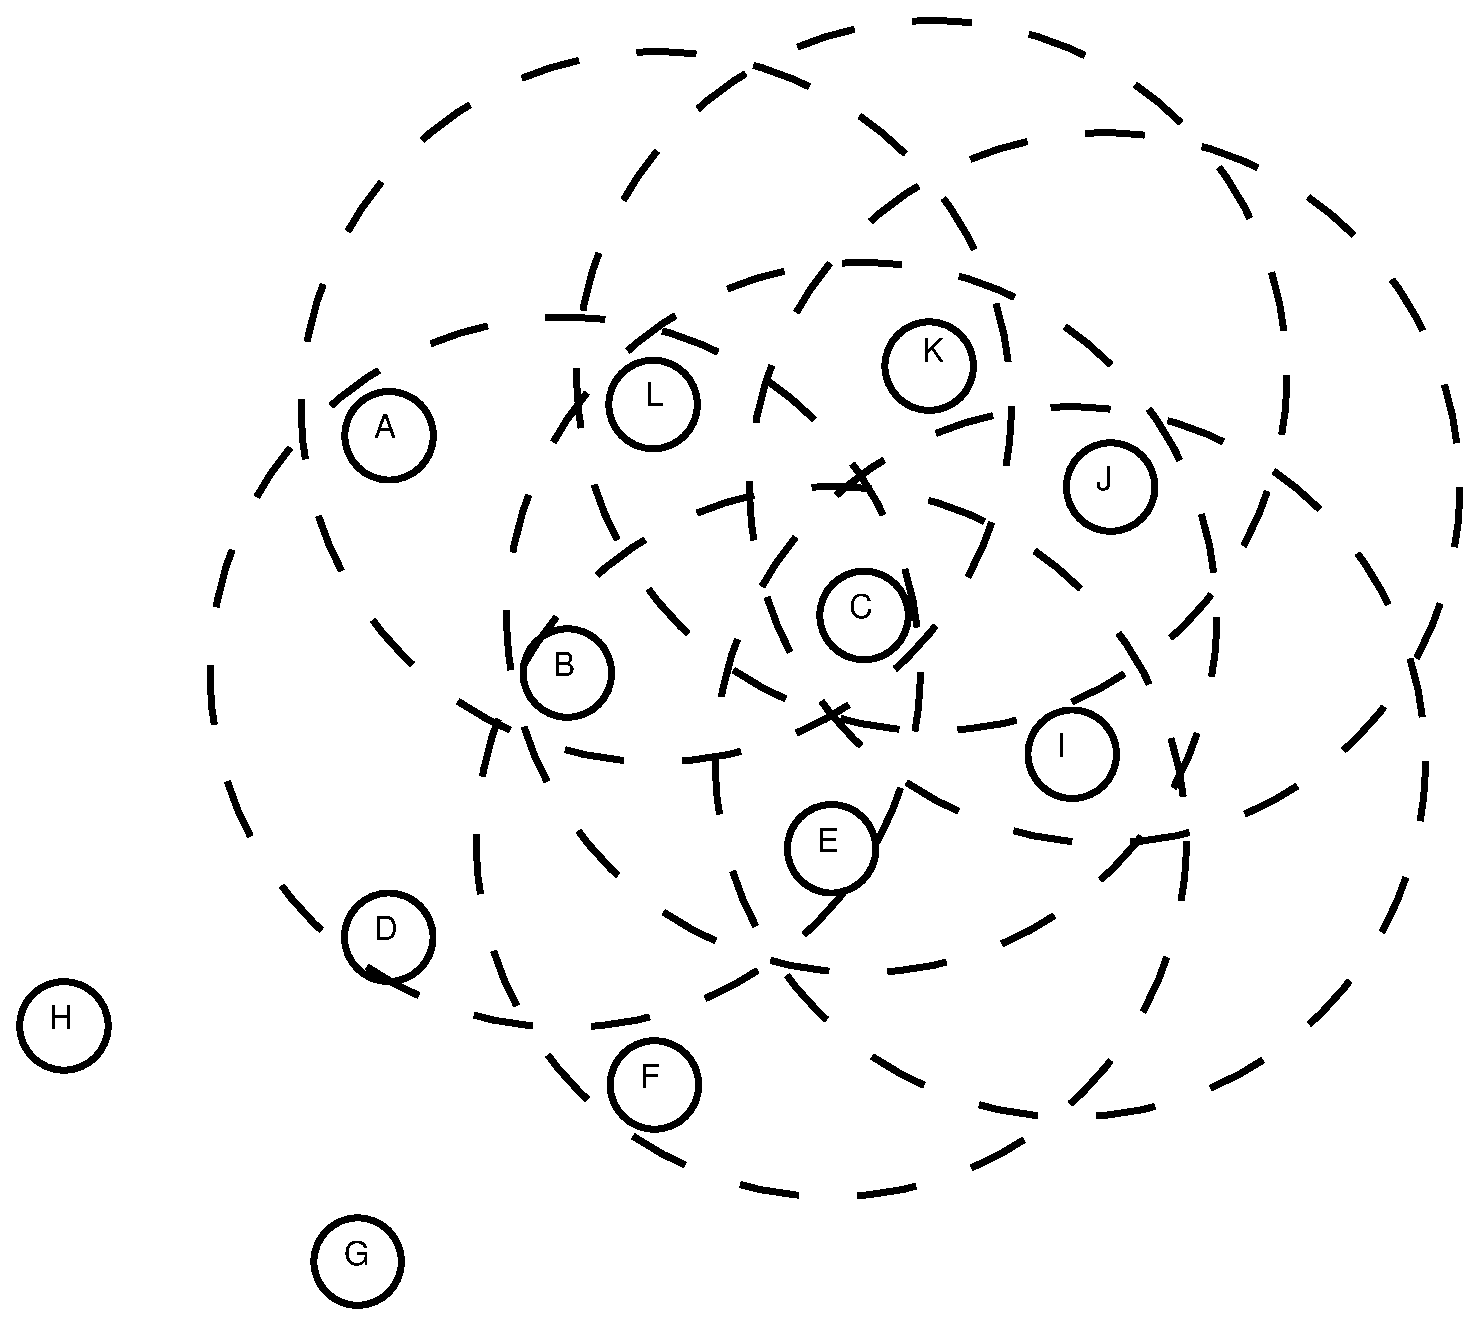
\includegraphics[width=0.7\textwidth]{ejemplonetslots.eps}
 \end{center}
 \caption{Neighbors, and neighbors from neighbors from \ac{AN} C}
 \label{fig:ejemplonetslots}
\end{figure}

In Figure \ref{fig:ejemplonetslots}, a network with 12 \acp{AN} is presented. These \acp{AN} have their coverage painted with a discontinuous line circle.
All \acp{AN} inside a circle are the neighbors of a determinate \ac{AN}. At the same time all these neighbor \acp{AN}, have their own coverage circles.
All \acp{AN} inside these circles and the ones before, cannot transmit at the same time as the first \ac{AN} to avoid hidden terminal problem, the others 
can without risk. In the Figure, \ac{AN} C has as neighbors \acp{AN} B, L, K, J, I and E, and these all have as neighbors the \acp{AN} A, D and F. All these
\acp{AN} cannot transmit at the same time as \ac{AN} C, but \acp{AN} H and G perfectly can.

Thanks to this slot reuse technique, the bigger the network the more optimal the slot distribution, finding that, when the number of \acp{AN} is not so big this 
technique almost does not help, as all \acp{AN} are inside the neighbor-neighbor distance. But when the number of \acp{AN} grows maintaining their density, 
the total needed slots are highly reduced.

To obtain the slot distribution automatically among all the \acp{AN} using this technique, the following algorithm is proposed:

\begin{itemize}
 \item First, a matrix with distances between \acp{AN} should be filled. In this matrix the number indicates the distance between
two \acp{AN} in the network. 1 indicates the \acp{AN} are neighbors, 2 indicates that one \ac{AN} is the neighbor of a neighbor, and so on. For 
the previous network example in Figure \ref{fig:ejemplonetslots}, Table \ref{tab:neighborsmatrix} is extracted.

\begin{table}
 \begin{center}
  \begin{tabular}{c|c|c|c|c|c|c|c|c|c|c|c|c|}
   %\noalign{\vspace*{0.5cm}}
   & \textbf{A} & \textbf{B} & \textbf{C} & \textbf{D} & \textbf{E} & \textbf{F} & \textbf{G} & \textbf{H} & \textbf{I} & 
    \textbf{J} & \textbf{K} & \textbf{L} \\
   \hline
   \textbf{A} & X & 1 & 2 & 1 & 2 & 2 & 2 & 2 & 3 & 3 & 2 & 1 \\
   \hline
   \textbf{B} & 1 & X & 1 & 1 & 1 & 1 & 2 & 2 & 2 & 2 & 2 & 1 \\
   \hline
   \textbf{C} & 2 & 1 & X & 2 & 1 & 2 & 3 & 3 & 1 & 1 & 1 & 1 \\
   \hline
   \textbf{D} & 1 & 1 & 2 & X & 2 & 1 & 1 & 1 & 3 & 3 & 3 & 2 \\
   \hline
   \textbf{E} & 2 & 1 & 1 & 2 & X & 1 & 2 & 3 & 1 & 2 & 2 & 2 \\
   \hline
   \textbf{F} & 2 & 1 & 2 & 1 & 1 & X & 1 & 2 & 2 & 3 & 3 & 2 \\
   \hline
   \textbf{G} & 2 & 2 & 3 & 1 & 2 & 1 & X & 1 & 3 & 4 & 4 & 3 \\
   \hline
   \textbf{H} & 2 & 2 & 3 & 1 & 3 & 2 & 1 & X & 4 & 4 & 4 & 3 \\
   \hline
   \textbf{I} & 3 & 2 & 1 & 3 & 1 & 2 & 3 & 4 & X & 1 & 2 & 2 \\
   \hline
   \textbf{J} & 3 & 2 & 1 & 3 & 2 & 3 & 4 & 4 & 1 & X & 1 & 2 \\
   \hline
   \textbf{K} & 2 & 2 & 1 & 3 & 2 & 3 & 4 & 4 & 2 & 1 & X & 1 \\
   \hline
   \textbf{L} & 1 & 1 & 1 & 2 & 2 & 2 & 3 & 3 & 2 & 2 & 1 & X \\
   \hline
  \end{tabular}
  \caption{\ac{AN} distances matrix}
  \label{tab:neighborsmatrix}
 \end{center}
\end{table}
To fill in this matrix, first all number ones have to be filled in (neighbors). Once this is done, all the twos, then all the threes \ldots. For 
example if A - B is 1 and B - C is 1, and A - C was left empty, then A - C will be 2.
 \item After the matrix is completely filled in, it begins slot assignation. First slot is assigned to first row \ac{AN}, in our case A. To 
make it easier, the algorithm will be explained based on the example as it is complicate enough to show all circumstances.
\begin{quote}
 Slot 1 - A
\end{quote}
Then, A row is covered from left to right until a number 3 or bigger is found, then this \ac{AN} gets the same slot as A, in this case I.
\begin{quote}
 Slot 1 - A, I
\end{quote}
Continuing the row, it is found that also J has a number 3, but as I and J have only a 1, they are not compatible and therefore J is left out. 
Then, next row is analyzed and B gets a slot.
\begin{quote}
 Slot 1 - A, I \\ Slot 2 - B
\end{quote}
It can be seen that B row has no numbers above 2. This means B cannot share a slot with any other \ac{AN} as it is so close to all of them. 
This makes sense, because as it can be seen in Figure \ref{fig:ejemplonetslots}, B is in the middle of the network. Next row C, gets another
slot and shares it with G but not with H for the same reason as A, I and J.
\begin{quote}
 Slot 1 - A, I \\ Slot 2 - B \\ Slot 3 - C, G
\end{quote}
Next row is D, this \ac{AN} gets its own slot, and covering the row, it is found that I can share the slot with it. But as I was already 
assigned and to allow other \acp{AN} to get also a slot, I is skipped and left for the end. This way, J is the next with number 3 or more 
which was not assigned yet, so it gets to share slot with J. There is still K with 3 or more, but K and J are not compatible, so K is left out.
We had still I to recheck, in this case it is no more compatible with J and it is therefore left out, but if it was compatible with all the 
\acp{AN} in the slot list, then I would get another slot. Based on this, \acp{AN} can get more than one slot if possible, and this way 
idle listening in the \acp{MN} gets reduced.
 \begin{quote}
  Slot 1 - A, I \\ Slot 2 - B \\ Slot 3 - C, G \\ Slot 4 - D, J
 \end{quote}
The matrix analysis continues as described until G row is reached. As G was already assigned, G is skipped and it does not get an extra 
slot like all the \acp{AN} did before. It happens the same with rows H, I, J and K. The current slot assignation is then like follows:
 \begin{quote}
  Slot 1 - A, I \\ Slot 2 - B \\ Slot 3 - C, G \\ Slot 4 - D, J \\ Slot 5 - E, H \\ Slot 6 - F, K
 \end{quote}
Row L. As L did not get a slot before, a new slot is assigned, and covering the row, the first number above 2 found is for G, but
like it was explained before, G has already a slot assinged and for that reason it is left for the end. H has also a 3 with L, but H 
was also assigned before and it is also left for the end.

As the end of the row was reached, and no other \ac{AN} was found to share the slot with L. The skipped list has to be checked. In this case 
the list has more than one element. To assure that all the \acp{AN} get the most slots they can, this list is ordered from the \ac{AN} with 
less slots assigned at the first place to the \ac{AN} with more slots assigned at the last place. This way, it is avoided for example, that 
an \ac{AN} gets one slot and another one three, when both could take two. In this case both G and H have only one slot assigned, that is why any 
of the two \acp{AN} gets the slot. For our example, G was chosen.

This is the final slot distribution:
 \begin{quote}
  Slot 1 - A, I \\ Slot 2 - B \\ Slot 3 - C, G \\ Slot 4 - D, J \\ Slot 5 - E, H \\ Slot 6 - F, K \\ Slot 7 - L, G
 \end{quote}
\end{itemize}

From this example, it can be seen that if \textit{syncPacketsPerSyncPhase} = 3, instead of having $12 \cdot 3 = 36$ slots in every Sync Phase, the slot 
number was reduced to $7 \cdot 3 = 21$ slots, reducing quite a lot listening time in the \acp{MN}.

The word slot was mentioned quite a lot, but how long is an slot?

From Figure \ref{fig:MACFrame} on page~\pageref{fig:MACFrame} and Figure \ref{fig:PPDU} on page~\pageref{fig:PPDU} it is obtained that \ac{MAC}
Layer header has 104 bits. And \ac{PHY} Layer header has 48 bits. If the Application Layer Sync Packet has the following structure:
\begin{itemize}
 \item[-] 8 bit: status
 \item[-] 32 bit: next phase start time-stamp
 \item[-] 16 bit: X dimension from \ac{AN} position
 \item[-] 16 bit: Y dimension from \ac{AN} position
 \item[-] 16 bit: Z dimension from \ac{AN} position
\end{itemize}
Making the \ac{MAC} Layer Payload 88 bits. This together with the 104 bits and the 48 bits, sums a total of 240 bits per Sync Packet to be sent.

As it was commented in Chapter \ref{chap:802154standard}: \nameref{chap:802154standard}, the bit rate is 250 Kbits/s. Therefore the Sync
Packet needs 0.96 ms to be transmitted. To this time, it has to be added the \ac{CCA} time and the \textit{aTurnaroundTime}. Adding to all this
a security gap in case of bad synchronization, make the slot length 1.5 ms.

To get good results from this technique, a good \acp{AN} distribution is of vital importance. \acp{AN} should be distributed with a density that all
\acp{MN} in the network, no matter where they are, can reach at least three \acp{AN}, but not so concentrated that all \acp{AN} can
reach each other to allow this technique to reduce the slots number. Whenever a wall or obstacle is found in the network, it could be modeled as
a reduction of the affected \acp{AN} coverage in this direction. 

As all this planning process would be done the first time the network is deployed and probably not changed anymore, the effort will just be made 
at the beginning and it will get compensated with a much better network performance than for the random case. This will be proved in Chapter 
\ref{chap:simulationandresults}: \nameref{chap:simulationandresults}.
\clearpage{\pagestyle{empty}\cleardoublepage}
\chapter{Protocol Implementation}
\label{chap:protocolimplementation}

This chapter details the simulation environment where the presented High Configurable Protocol was developed and tested. Simulation was chosen 
instead of analytical study or real networks, because this are difficult or expensive for such a complex protocol. During this chapter a 
deeper view into the protocol will be given, as all generated code will be explained in detail.

\section{Used Tools}

To develop this project different simulators and frameworks were considered, choosing finally \ac{OMNeT++} 4.0 \cite{OMNeT}
as simulator, and \ac{MiXiM} 2.0 \cite{MiXiM} as framework, due to its versatility, their short time to get to work with them for the first time and 
their current development of 802.15.4 standard, specially in non-beaconed mode.

After all simulations were done, the results were extracted with a tool called \textit{scavetool}. This data is than imported and treated with 
\ac{MATLAB} \cite{MATLAB} to obtain all results in Chapter \ref{chap:simulationandresults}: \nameref{chap:simulationandresults}.

\subsection{\ac{OMNeT++} 4.0}

\ac{OMNeT++} 4.0 is an object oriented discrete event simulator, based in C++ \cite{cpp}. \ac{OMNeT++} consists in several modules hierarchically
connected and that communicate among them through messages. Modules relation is done through an own easy programming language called \ac{NED}.
This language is written in the \textit{.ned} files. This files, apart from relations among modules, contain parameters about them. The value for this
parameters can be given directly in the \textit{.ned} file or also in a file called \textit{omnetpp.ini}, that is the network configuration file.
This file's contain is basically simulation configuration parameters and module parameter values.

This software allows two kind of simulation environments, a graphic one (Tkenv) and a command line one (Cmdenv). Working with the graphic one, 
message interchange simulation can be done step by step, this mode is good to debug the code.

The command environment, allows to make express simulations in order to obtain the final results much faster than for graphic environment. In this 
mode it is possible to simulate changing parameters and also make several repetitions, this is all automatically done, not requiring the user intervention.
This mode makes all the process much easier when lots of iterations must be done. When random numbers are used, they are generated depending on a seed. 
This seed can be defined by the user but can also depend on a parameter, it usually changes with the run number. As this seed will be the same for the
same run number, all generated random numbers and hence the results will also be the same. This fact makes \ac{OMNeT++} a powerful tool in debugging 
process.

All modules in \ac{OMNeT++} are executed theoretically in a concurrent way, usually computers have only one processor so this is not always
practically possible. Anyway, it should be kept in mind that when a module depends on other module's data, the data should be taken at a 
later moment, if it is done at the same moment, data might not be ready.

All \ac{OMNeT++} modules have the same structure as they inherit all from the same class \textit{cSimpleModule}, later on, some modules could 
implement new methods, but they all have this basic ones:

\begin{itemize}
 \item \textbf{initialize - }This method is executed for every module by the \ac{OMNeT++} core  at the beginning of the simulation, and only there 
(time T = 0). This method gets as parameter the variable \textit{stage}. This parameter goes from 0 until the number defined by the method 
\textit{numInitStages()}.

It was said before that all modules in \ac{OMNeT++} are executed concurrently. This means that it cannot be assured that \textit{initialize} method from 
a module will be executed before the one for another module. If there is a data dependency between modules in this method, it should be solved
manually calculating the data in a smaller \textit{stage} than the one where the data will be read. Thus, if network needs to be initialized in an 
specific order, this should be done separating code among all the different \textit{stages}. First, all 0 \textit{stages} will be executed, then all 
1 \textit{stages}, etc. until the number defined for each module.

During this phase, it should be sent at least a message in at least one of the modules of the network, otherwise, the network will not start doing 
anything.
 \item \textbf{finish - }This method stores all the desired results at the end of the simulation. This results could be any of the variables during the 
simulation. This method should not delete the variables, that should be done in the class destructor.
 \item \textbf{handleMessage - }This method is the one executed each time a message arrives to a module. All modules are connected through gates,
being in this work usually the ones showed in Figure \ref{fig:omnetmodule}. Messages who arrived to a module, could come from one of the gates or be a self
message. Usually this method calls another methods that take care of the message depending if it is a self message (usually used to schedule 
tasks in a future time), a data message or a control message. This methods are: \textit{handleSelfMsg, handleUpperMsg, handleLowerMsg, 
handleLowerControl and handleUpperControl}.
\begin{figure}[ht]
 \begin{center}
  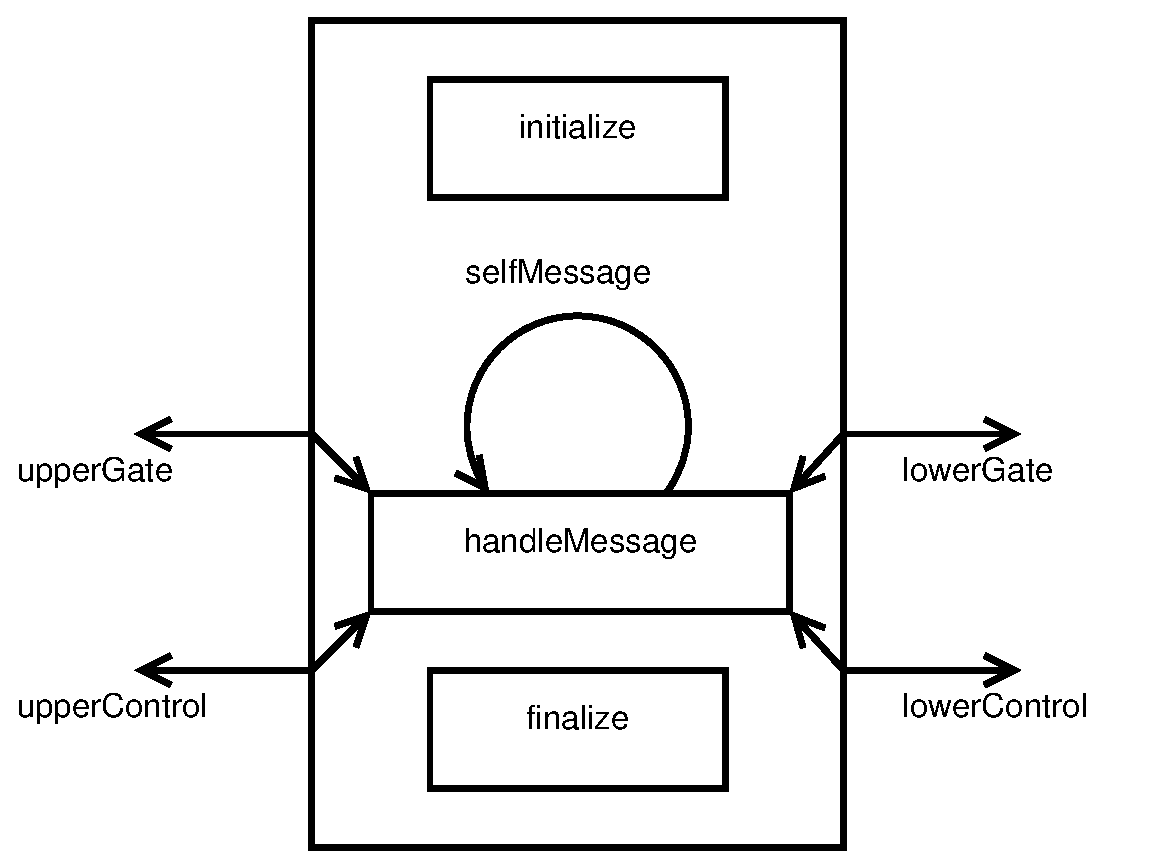
\includegraphics[width=0.5\textwidth]{omnetmodule.eps}
 \end{center}
 \caption{Basic \ac{OMNeT++} module structure}
 \label{fig:omnetmodule}
\end{figure}
 \item \textbf{sendDown/sendUp/sendControlDown/sendControlUp }This methods send a message from a module through the already commented gates.
 \item \textbf{scheduleAt - }This method schedules a self message in a certain time in the future. This is useful when programming timers or when a
message should be sent with a delay.
 \item \textbf{decapsMsg/encapsMsg - }Usually before a message is sent from one layer to another in the same device, it should be encapsulated or 
decapsulated. When this is done, instead of message, it is talked about packet. \textit{Packet} is a class that inherits from class \textit{message}. It 
is also possible to define a custom packet (check \cite{manualomnet} for this).
\end{itemize}

This methods and no others, were commented because they are going to be used many times during the work. For more information about \ac{OMNeT++}, 
refer to the user manual \cite{manualomnet}.

\subsection{\ac{MiXiM} Framework}

\ac{MiXiM} 2.0 framework provides \ac{OMNeT++} with many new modules. Among them, all necessary modules to work with 802.15.4 Standard. 
All this modules are build following \cite{IEEE802.15.4-2006}.

The basic structure of a node in \ac{MiXiM} is like shown in Figure \ref{fig:miximmodule}. This figure shows already some new modules added by
this work to the basic \ac{MiXiM} node. Depending on the kind of node: Computer, \ac{AN} or \ac{MN}, the \textit{.ned} files will load 
different modules to describe each behavior. This files should be also checked if a complete list of parameters is needed.

\begin{figure}[ht]
 \begin{center}
  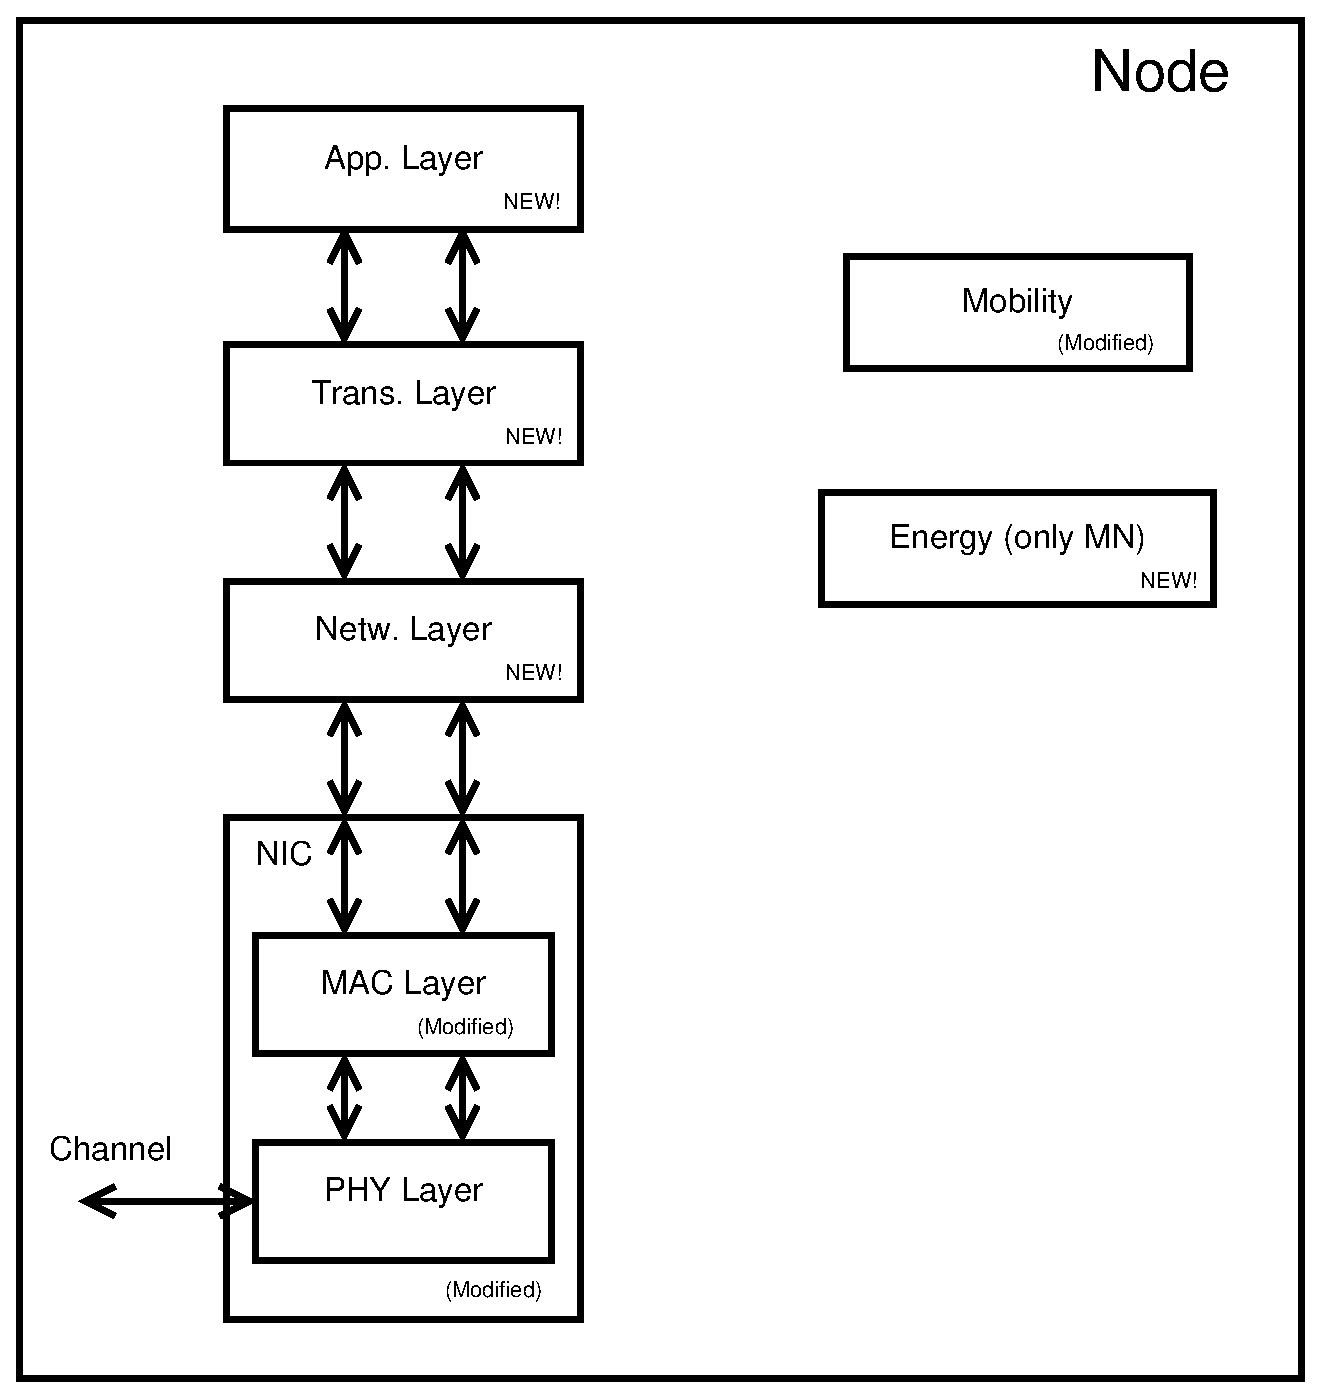
\includegraphics[width=0.8\textwidth]{miximmodule.eps}
 \end{center}
 \caption{Basic \ac{MiXiM} node structure}
 \label{fig:miximmodule}
\end{figure}

In this sub-section, only modified \ac{MiXiM} original modules will be commented leaving the new implemented modules for the next sub-sections.

\subsubsection{New packet structure}
\label{sec:packetstructure}

In \ac{OMNeT++}, there are special files (\textit{.msg}) that define messages types. When the project is compiled, a class is automatically 
generated from every \textit{.msg} file. \ac{MiXiM} contributes \ac{OMNeT++} with many different message files. One of this files is the 
\textit{ApplPkt.msg}. This packet will be generated in the Application Layer and encapsulated in every layer until it gets transmitted into the 
air. For this work, this packet should include the following information that it did not before:
\begin{itemize}
 \item \textit{realDestAddr} and \textit{realSrcAddr}. This values are better explained with an example. When a \ac{MN} sends a report to the 
computer, the first step is sending the report to the selected \ac{AN}, this will be the \textit{destAddr} but the report is really intended
to go until the computer, this is the \textit{realDestAddr}. When this report arrives at the computer, for it, the \textit{srcAddr} is the 
address of the selected \ac{AN}, and the address of the \ac{MN} would be the \textit{realSrcAddr}.
 \item \textit{retransmisionCounterBO} and \textit{retransmisionCounterACK}. Whenever the \ac{MAC} Layer informs the Application Layer that a 
packet was dropped, Application Layer checks if there are still more retransmission available for this packet. Counter
\textit{retransmisionCounterBO} is used to check the case when packet was dropped due to a maximum number of Backoffs, and counter 
\textit{retransmisionCounterACK} is used to check the case where the packet was dropped because no \ac{ACK} was received. This counters are
increased by Applicaton Layer whenever a packet is retransmitted.
 \item \textit{CSMA}. This variable is a boolean, and if it is true, indicates the \ac{MAC} Layer that \ac{CSMA/CA} has to be disabled for 
this packet.
 \item \textit{askForRequest} and \textit{requestPacket}. This two variables are also booleans. When \textit{askForRequest} is true, it means
that \ac{MN} wants to notify the selected \ac{AN} that in the next period a data will be asked for. When \textit{requestPacket} is true, it
measn that \ac{MN} requests some information to the selected \ac{AN}. This flags are here to help the selected \ac{AN} to know what kind of 
report is receiving.
\end{itemize}

This packet structure is just for simulation purposes and has nothing to do with the real packet structure and hence with the size of the 
packet (\textit{bitLength} from \textit{cMessage} class) to be sent in the channel. Apart from Application Layer packet, \ac{MAC} and 
\ac{PHY} Layer will add their own headers. From Figure \ref{fig:MACFrame} on page~\pageref{fig:MACFrame} and Figure \ref{fig:PPDU} on 
page~\pageref{fig:PPDU} it is obtained that \ac{MAC} Layer header has 104 bits. And \ac{PHY} Layer header has 48 bits. This \ac{MAC} Layer
header size, assumes both addresses as short addressed, but in case a report has its origin or destination in a \ac{MN}, a long address 
must be used. This 6 bytes difference will be compensated adding them to Application Layer packet size.

According to Application Layer, the following real packets can be distinguished:
\begin{itemize}
 \item \underline{Sync Packet}. Has 1 byte for the status, 4 bytes for the next phase time-stamp and 2 + 2 + 2 bytes for \ac{AN} position. 
Its size is hence 88 bits.
 \item \underline{Normal Report}. Reports the listened \acp{RSSI} during the previous Sync Phases. It has 1 byte for the status and 2 bytes 
for each listened \ac{AN}. This report only exists for \acp{MN} in modes 1 and 4. As the source address is a \ac{MN}, 6 bytes have to be added.
Its size is hence $56 + 2\cdot X$ bits, where X is the number of \acp{AN} where a Sync Packet was listened to.
 \item \underline{\ac{MN} in mode 2 Report}. Reports the calculated positions from itself. It has 1 byte status and $2 + 2 + 2 = 6$ position 
bytes for each position calculated (maximum five). This report exists only for \acp{MN} in mode 2. As the source address is a \ac{MN}, 6 bytes 
have to be added. Its size is hence $56 + 6\cdot X$ bits, where X is the number of calculated positions to transmit.
 \item \underline{Ask Report}. Report or extra report with the ASK flag activated. In this case, 10 bytes are added to the report where the
flag is activated. This 10 bytes represent the information needed by the selected \ac{AN} to know which data the \ac{MN} is asking for.
 \item \underline{Request}. Report or extra report with the Request flag activated. In this case, 1 byte is added to the report where the
flag is activated. This byte shows which information was requested.
 \item \underline{\ac{MN}'s broadcast}. Broadcast packet sent by \acp{MN} in modes 3 and 4. It has 1 byte for the status and 1 byte information.
As the source address is a \ac{MN}, 6 bytes have to be added. Its size is hence 64 bits.
 \item \underline{\ac{AN}'s answer to request}. Report sent by \acp{AN} when answering a \ac{MN}'s request. It has 1 byte status and 10 bytes info.
As the destination address is a \ac{MN}, 6 bytes have to be added. Its size is hence 136 bits.
 \item \underline{Broadcasts collection packet}. Report sent by an \ac{AN} as collection of all broadcasts received from a \ac{MN} in mode 3 
or 4. It has 1 byte status, 2 bytes for \ac{RSSI} info and 6 bytes for showing which \ac{MN} the \ac{RSSI} belongs to. Its size is hence 72 bits.
\end{itemize}

\subsubsection{Connection Manager}

Apart from node structure modules, there is a central module in \ac{MiXiM}, called \textit{connectionManager}. This module is in charge of connecting
all nodes at a reachable distance. It keeps a list of all nodes and it is called every time a node changes its position. \textit{ConnectionManager} 
updates then the position in the list and recalculates all connections. The maximum distance where two nodes could still reach each other, is 
calculated using the transmit power and sensitivity, both are defined in \textit{omnetpp.ini}.

Each element from the node list is an object of the class \textit{NicEntry}. This class stores among many other data, the coordinates where the node is.
This class was modified to store also the following data:

\begin{itemize}
 \item \underline{Module Type}. It stores in the variable \textit{moduleType} the node type this \ac{NIC} belongs to. The values could be 1 for \ac{AN}, 
2 for \ac{MN} and 3 for Computer. Its value is assigned when initializing the node. As defining this variable here, it can be read from all modules in the 
network. This is useful to make lists of the different types of nodes.
 \item \underline{Slot Information}. Through variables \textit{transmisionSlot} and \textit{numSlots}, the \ac{AN} knows which slots of the 
\textit{numTotalSlots} are the ones reserved for it to transmit. All this three variables are assigned by the Computer in its \textit{initialize} method.
\end{itemize}

\subsubsection{Mobility module modifications}

The mobility module is the responsible of the node's positions. It is the one assigning the initial position to the nodes and it is also the one
used whenever a node wants to be moved. This module's functionality is described in class \textit{BaseMobility}. As the position of the nodes is needed,
this class is also linked with the \textit{NicEntry} class. Unlike \textit{connectionManager}, this is not a general module, and each node have their own
mobility node as it can be seen in Figure \ref{fig:miximmodule}.

During \textit{initialize} method in \textit{BaseMobility}, all node's initial positions, are assigned according to the values given in the file
\textit{omnetpp.ini}. A different value for each coordinate (X, Y, Z) must be given, and all of them must be inside the playground area (defined also
in \textit{omnetpp.ini}). When instead of a fixed value for the position, a ``-1'' is given, node will get a random position. The modifications done to
this class, refer precisely to the node's initial position assignment.

\begin{itemize}
 \item \underline{Uniform random distribution}. It was already seen that assigning ``-1'' as value for a node's coordinate, this coordinate will be 
randomly assigned. But if all coordinates are ``-1'', a new peace of code at \textit{stage} = 2 during \textit{initialize} method is executed. This 
code distributes \acp{AN} and \acp{MN} uniformly and randomly in the playground according to \textit{minimumDistanceAnchor} and 
\textit{minimumDistanceNode} parameter respectively. This two variables represent, as their names show, the minimum distance to leave among \acp{AN} 
and the minimum distance to leave among \acp{MN}.
 \item \underline{Grid distribution}. When ``-2'' is assigned to all \ac{AN}'s coordinate values in \textit{omnetpp.ini}, all \acp{AN} will be 
distributed all over the playground forming a grid. The dimensions of the grid will depend on the number of \acp{AN}, resulting for example for 25 
\acp{AN} a 5 x 5 grid. This grid distribution, will be done at \textit{stage} = 0 during \textit{initialize} method.
\end{itemize}

\subsubsection{\ac{MAC} Layer modifications}
\label{sec:macmodifications}

\ac{MAC} Layer for 802.15.4 in \ac{MiXiM} is defined by the \textit{csma} class. This class works as a \ac{FSM} which diagram is as shown in Figure 
\ref{fig:csmaFSM}.

\begin{figure}[ht]
 \begin{center}
  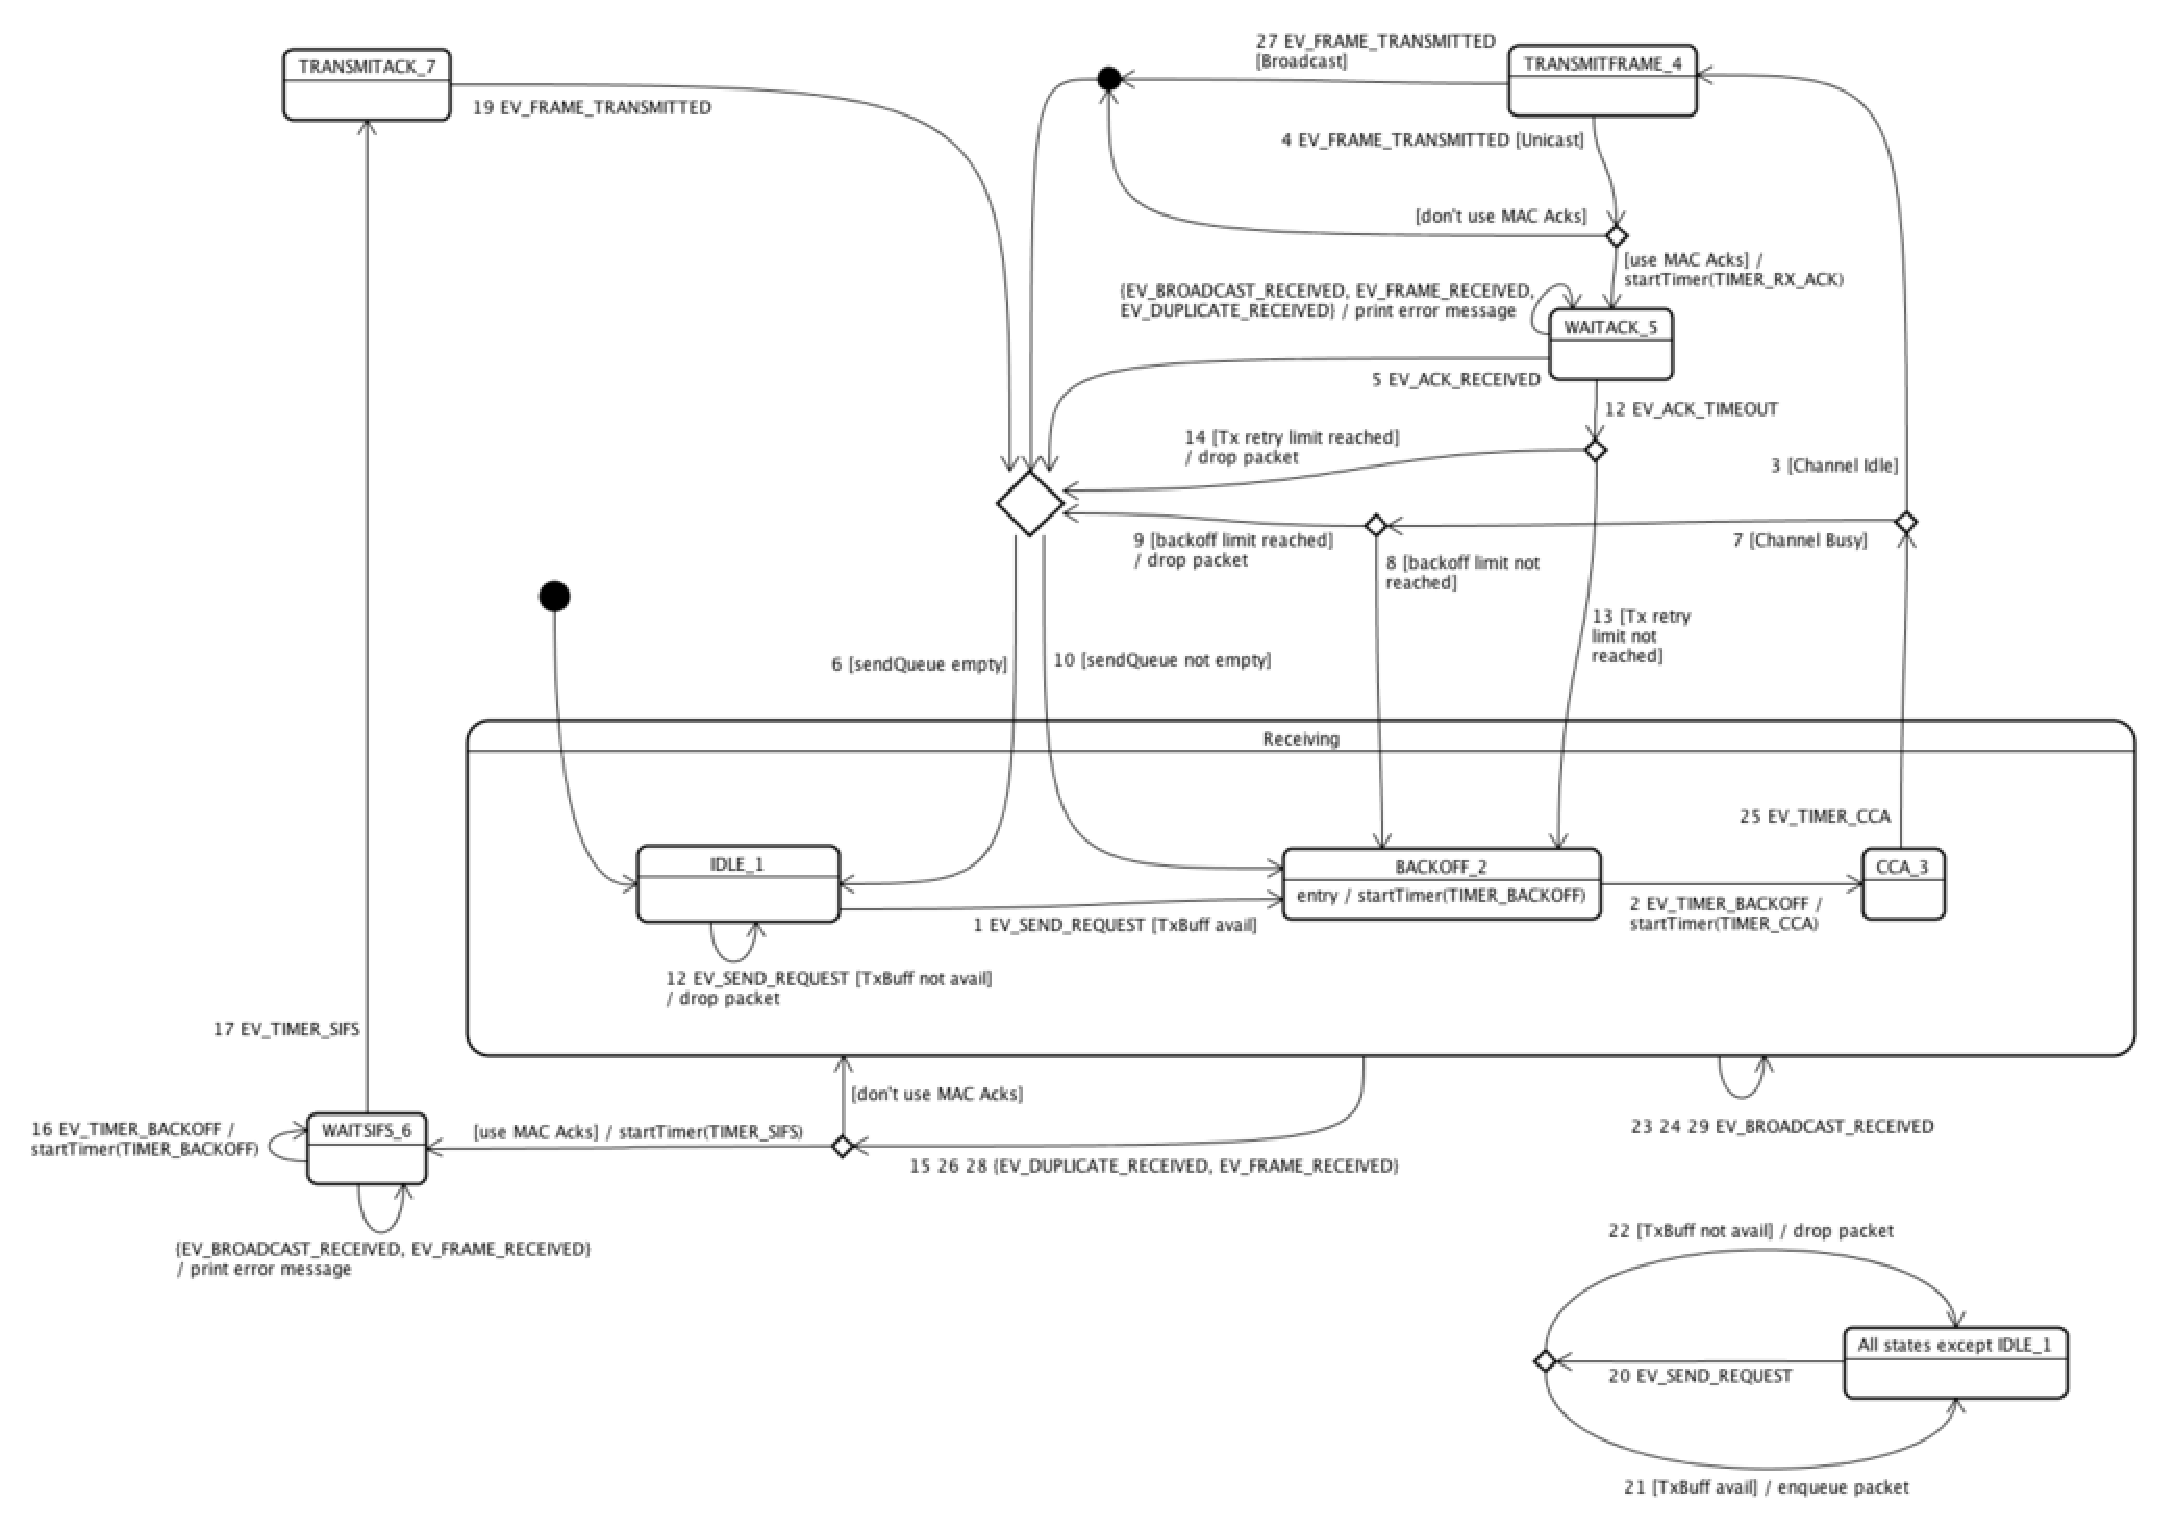
\includegraphics[width=1\textwidth]{csmaFSM.eps}
 \end{center}
 \caption{\ac{MiXiM}'s 802.15.4 \ac{MAC} Layer \ac{FSM} diagram \cite{MiXiM}}
 \label{fig:csmaFSM}
\end{figure}

Modifications done to this class are:

\begin{itemize}
 \item \underline{\ac{CSMA/CA} disable possibility}. During method \textit{updateStatusIdle} and whenever there is a packet in \ac{MAC} queue to
be transmitted, the first Backoff time would be calculated. In case the \ac{CSMA/CA} is deactivated, instead of calculating the first Backoff
time and scheduling the \ac{CCA} at this time, \ac{CCA} will be scheduled after \ac{SIFS} seconds (to assure Radio is in Rx state). If after the
\ac{CCA}, the channel is busy, the packet must be directly discarded instead of calculating a second Backoff time, that is why the \ac{NB} is 
set to the maximum number of retries. 
 \item \underline{Protocol phases end control}. It was added a way to control in which phase the node is, this control is started during the
\textit{initialize} method at stage 4 and it is rescheduled for every phase from method \textit{handleSelfMsg}. This control makes that the 
\ac{MAC} Layer, at the beginning from every phase, checks if the \ac{MAC} queue has elements from previous phase, in this case this elements
are erased and the number of elements recorded to have it as a result when calling the \textit{finish} method.

Before the end of every phase, it is left a \textit{guardTransmitTime} time. When \ac{MAC} Layer tries to send next packet in the queue, if the end of 
the first Backoff time goes beyond the guard time, this packet is not scheduled but it is erased. This erased packets number is also recorded
to be extracted as a result. This guard time for our work is 10 ms, it is this long to be protected even against the biggest packets during the 
simulation.
 \item \underline{Energy management}. In \ac{MiXiM}, although \ac{PHY} Layer has a SLEEP state, it is never used. This work has made \acp{MN}
going to sleep whenever they are able to. As this will be treated in Section \ref{sec:frameworkdevelopment} (\nameref{sec:frameworkdevelopment})
in a deeper way, here it would be just commented that whenever a \ac{MAC} state or a \ac{PHY} state gets changed in \textit{csma} class, another
class called \textit{energy} has to be warned.
 \item \underline{New control messages}. Before the modifications, \textit{csma} class informed upper layers whenever a sent report received an
\ac{ACK}, now, it informs also when broadcasts and \acp{ACK} were successfully sent to the channel. This class was also modified to 
report when a packet is dropped due to maximum number of Backoff retries, or to maximum number of ``no \ac{ACK} received`` retries, or when
\ac{MAC} Queue is full. Before it was only informing about packet dropped but without any reason. All this control messages will be treated 
in the Application Layer and they will be studied in following sections.
\end{itemize}

For a deeper view of \ac{MiXiM}'s \ac{MAC} Layer, a look up at \cite{MiXiM} and a deep view into the source code together with the diagram in Figure 
\ref{fig:csmaFSM} are recommended.


\section{Sync Phase study development}

Before constructing all the protocol framework, it had to be decided if during the Sync Phase the \acp{AN} would transmit their broadcasts 
synchronized in slots or randomly. For this purpose, a special and small framework was done, where just a simple Application Layer was added to 
the nodes. As this was just a temporary Application Layer, just the main aspects of it will be given.

\textit{Decider802154Narrow} class was modified to disable errors caused by noise and random errors due to the channel, this features were 
again enabled for the protocol framework development. This way whenever there is a fail, it can be known that it is due to simultaneous \ac{CCA}
or Hidden Terminal Problem.

\subsection{\ac{MN}}

\ac{MN} is the one receiving the broadcasts sent by the \acp{AN}. The only task for \ac{MN} is whenever it receives a broadcast, it stores in a
variable when and from which \ac{AN} the broadcast was. This way the performance could be later analyzed.

\subsection{Computer}

Computer does not really participate in the packet exchange, but it calculates the slot distribution among the \acp{AN} for the slotted case. 
Slot calculation is done according to the algorithm showed in Section \ref{subsec:slottedsyncphase} (\nameref{subsec:slottedsyncphase}). Computer 
also calculates the length of the different phases in the period. This length information is needed when packets are randomly transmitted 
during Sync Phase to compare with the slotted case, otherwise the maximum time to transmit will not be known. Slots calculation is done at
\textit{stage} 3 during \textit{initialize} method in \textit{ComputerAppLayer} class.

\subsection{\ac{AN}}

\acp{AN} are the responsible to send the broadcasts to be detected by the \ac{MN}. Depending on the mode (slotted or random) the 
behavior changes:
\begin{itemize}
 \item \underline{Random}. The first random broadcast gets scheduled at \textit{stage} 4 during \textit{initialize} method in \textit{AnchorAppLayer}
class. It gets scheduled a random time after starting the simulation. This random time has a maximum value defined in 
\textit{syncFirstMaxRandomTime}. Every time a message is sent, the next one is scheduled in a random time from this moment. This random 
time has also a maximum, but this time defined in \textit{syncRestMaxRandomTimes}. To make simulation easier, this two variables are going to get
always the same values.

The retransmission is done in \textit{handleLowerControl}
method whenever a broadcast was successfully sent in the channel and if the already sent broadcasts number is smaller than 
\textit{syncPacketsPerSyncPhase}. If on the other hand, the broadcast was not successfully sent into the channel, it is retransmitted, recording
it for the results.
 \item \underline{Slotted}. At \textit{stage} 4 during \textit{initialize} method, the first packet in the first slot is scheduled. This is done
in \textit{stage} 4 and not before, because all slot information is calculated by the computer in \textit{stage} 3. The next slotted packets to
send are scheduled during the \textit{handleSelfMsg} method. In this mode, the \textit{handleLowerControl} method has no functionality as all 
packets would be sent into the channel without problems. The number of slots per \ac{AN} during a Sync Phase, will be defined also by the variable 
\textit{syncPacketsPerSyncPhase}.
\end{itemize}


\section{Framework development}
\label{sec:frameworkdevelopment}

Apart from the modules already commented, the only ones to be introduced yet are the relatives to the node structure. This are the ones marked
with ''NEW$!$`` in Figure \ref{fig:miximmodule}. Due to their similarity among types of nodes and their simplicity, the modules 
\textit{Energy}, Transport Layer and Network Layer are going to be explained altogether. However, all Application Layers are going to be 
explained separately for \acp{AN}, \acp{MN} and Computer.

\subsection{Energy module}

Although this module is available for all types of nodes, it will be used just for \acp{MN}, as these are the nodes where the energy 
consumption is important. Whenever a \ac{MAC} or \ac{PHY} state is 
changed in \ac{MAC} or Application Layers, this module's main method will be called (\textit{updateStateStatus}). This class 
(\textit{EnergyConsumption}) will also \textit{initialize} with lots of default values and will \textit{finish} saving many different 
time values and calculating energy values to be studied later on.

In \ac{MiXiM}, \ac{PHY} Layer has no IDLE state. This work used hence the \ac{Rx} state to represent both \ac{Rx} and IDLE states. But this is
not 100\% correct because consumed energy in both states is not the same. That is why this module was created implementing its own state machine,
with the states SLEEP, \ac{Rx}, \ac{Tx} and IDLE. The transition among all the states can be observed in Figure \ref{fig:statesDiagramEnergy}. 
Inside the circles, with a bigger font, it is said the state of the \textit{Energy} module and with a smaller font, the equivalent \ac{MAC} 
states.

\begin{figure}[ht]
 \begin{center}
  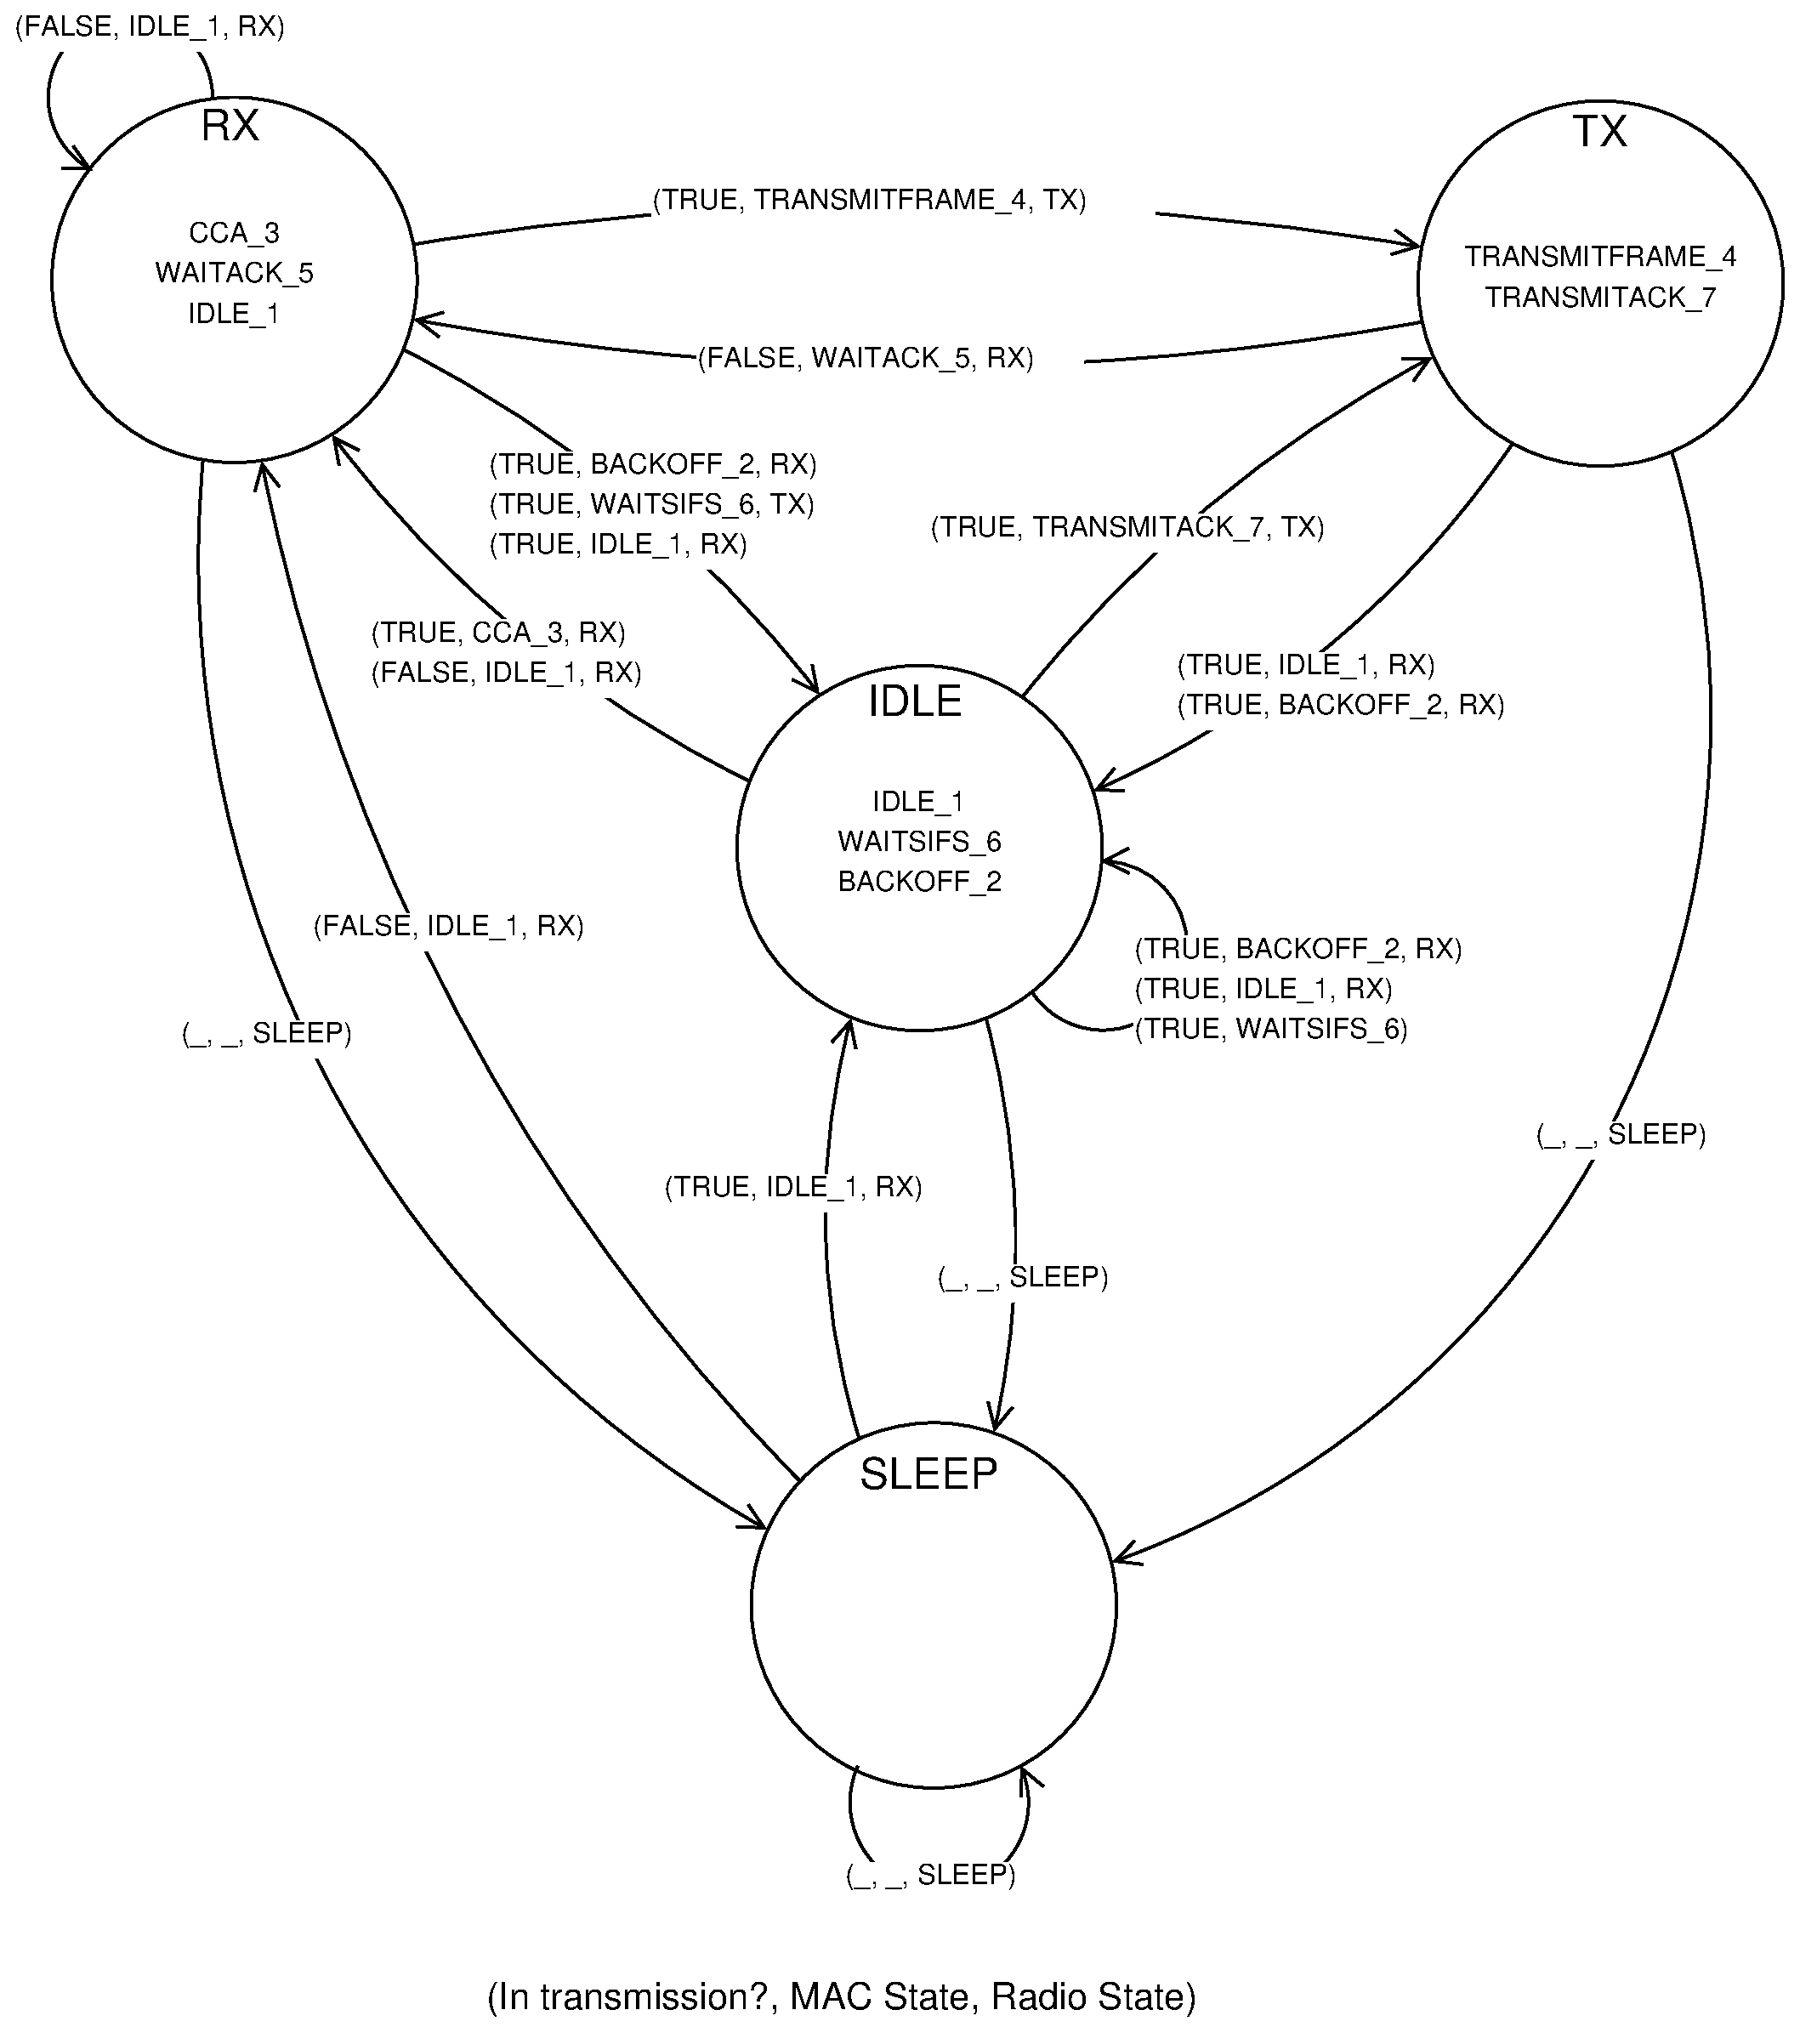
\includegraphics[width=0.8\textwidth]{statesDiagramEnergy.eps}
 \end{center}
 \caption{\textit{Energy}'s \ac{FSM} diagram}
 \label{fig:statesDiagramEnergy}
\end{figure}

Whenever there is a transition between two states, the three values between brackets on the figure (A, B, C), go also as argument of the 
\textit{updateStateStatus} method. When one of this values in the figure takes the \_ value, that means that the value sent
in this position is not important.

First value (A, \_, \_), is a boolean indicating true if the \ac{MN} is in a packet transmission process or false if it is in a IDLE or packet 
reception process. This might be important in some cases to differentiate when \ac{PHY} state \ac{Rx} is being used really as \ac{Rx} or as
IDLE.

Second value (\_, B, \_), indicates the \ac{MAC} state the \ac{MAC} Layer is changing to. Some times it is necessary to change \ac{PHY} Layer state
without modifying the \ac{MAC} state from the Application Layer. This Layer has no access to know in which state the \ac{MAC} Layer is. That is
why, when \ac{MAC} state does not want to be changed, the total number of \ac{MAC} states must be given.

Third value (\_, \_, C), indicates the \ac{PHY} state the Radio is changing to. For the same reason as before, the total number of \ac{PHY} states
could be given.

The main functionalities of \textit{updateStateStatus} method are:
\begin{itemize}
 \item Calculating and changing the new Energy State according to the previous state and the given arguments, following the diagram in Figure
\ref{fig:statesDiagramEnergy}.
 \item Calculating through time-stamps, the total time that \acp{MN} were in each state, as well as how much time was spent in all the different
transitions.
 \item Calculate the time the microprocessor spent calculating \ac{MN} position (\ac{MN} in Mode 2). During this time, transceiver
state and hence energy state are in SLEEP, but the microprocessor is working spending an energy that should be took into account.
\end{itemize}

\subsection{Transport Layer}

Transport Layer from Computer, \acp{AN} and \acp{MN} does not really do anything else than forwarding messages and control messages coming from 
Network Layer to Applications Layer and vice versa. This Layer was build to have its main structure available for a future work when 
aggregation and segmentation were needed as an idea to reduce traffic in the network. The three classes are \textit{ComputerTransLayer},
\textit{AnchorTransLayer} and \textit{NodeTransLayer} respectively.

\subsection{Network Layer}

As it was commented in Chapter \ref{chap:802154standard} (\nameref{chap:802154standard}), the topology of the network selected for this work,
is the tree topology. In this topology all \acp{AN} can communicate only whit their parents or children. On the top of this topology, is 
the computer.

A complicate routing protocol would be out of the scope of this project, that is why a network where all \acp{AN} do not change their positions 
in every simulation is needed. A grid topology was chosen because of its simplicity as well as because it is found in the literature quite often 
as a standard network where to try different protocols. For our work an scenario like the one in Figure \ref{fig:finalscenario} will be used 
in Chapter \ref{chap:simulationandresults} (\nameref{chap:802154standard}).

Assuming that the \acp{AN} are fixed and situated like shown in Figure \ref{fig:finalscenario}. The tree topology showed in Figure 
\ref{fig:routetree} is obtained. With this topology, a routing matrix could be easily extracted and stored in the nodes. This way nodes 
are able to know which next jump the packet should make to reach its final destination.

\begin{figure}[ht]
 \begin{center}
  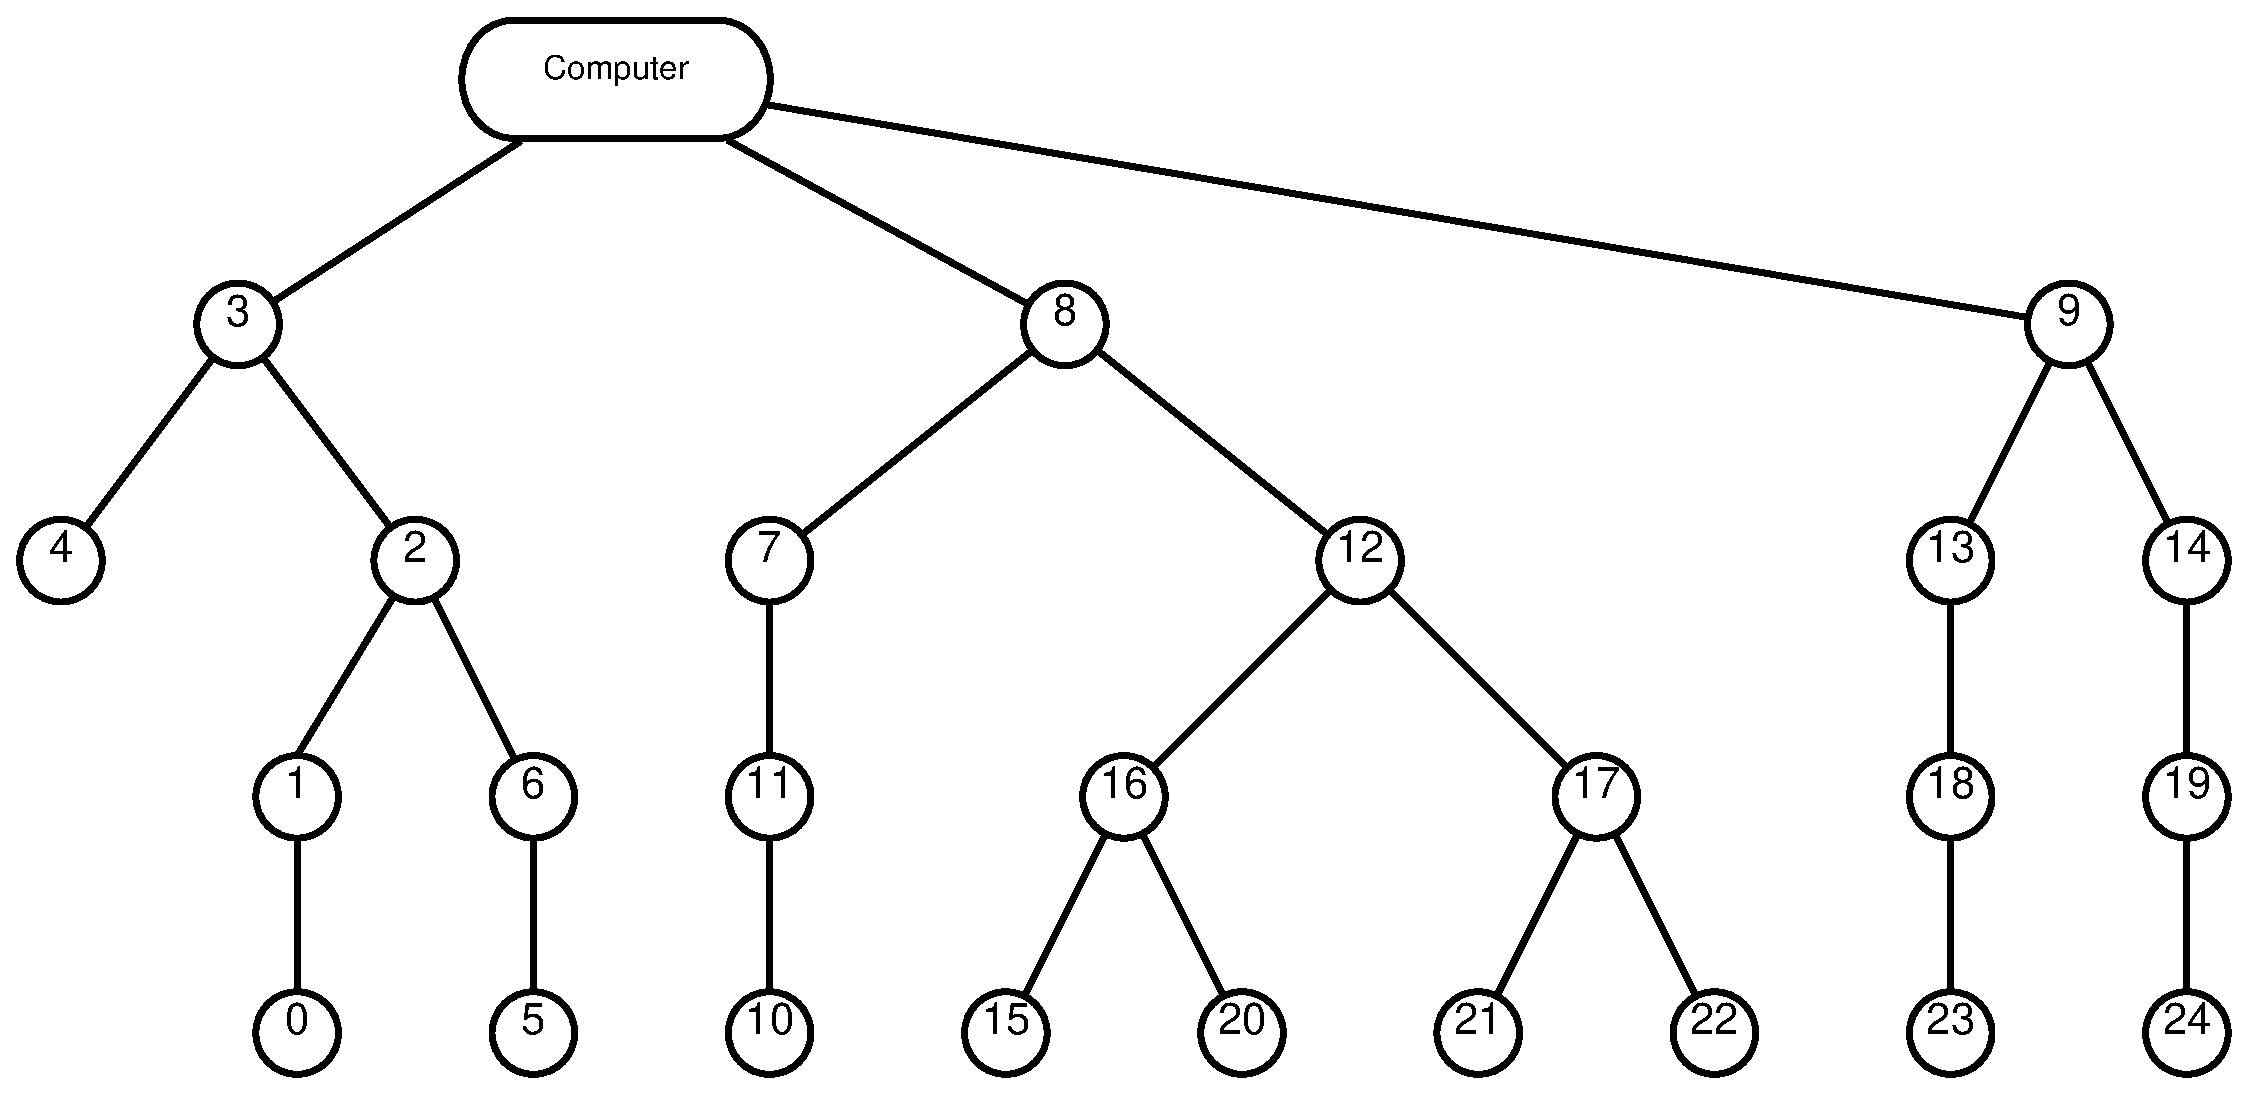
\includegraphics[width=0.8\textwidth]{routetree.eps}
 \end{center}
 \caption{Routing Tree Topology}
 \label{fig:routetree}
\end{figure}

Network Layer is present in the Computer, \acp{AN} and \acp{MN}, being the classes describing its functionality \textit{ComputerNetLayer},
\textit{AnchorNetLayer} and \textit{NodeNetLayer} respectively. All this classes have the same structure and their main methods are the following:
\begin{itemize}
 \item \textit{handleLowerControl}: this method receives a control message from \ac{MAC} Layer through Transport Layer and redirects it to the
Application Layer.
 \item \textit{handleUpperControl}: this method receives a control message from Application Layer and redirects it to the \ac{MAC} Layer through
Transport Layer.
 \item \textit{handleLowerMsg}: this method receives a message from \ac{MAC} Layer through Transport Layer, and after decapsulating it, sends it
to the Application Layer.
 \item \textit{handleUpperMsg}: this method receives a message from Application Layer and after encapsulating it, sends it to the \ac{MAC}
Layer through Transport Layer.
 \item \textit{encapsMsg}: this method adds (or encapsulates) a header to the Application message with the address of the next jump. This 
header will be however 0 bit long, because although the address is calculated here, it is only encapsulated to provide it to the \ac{MAC} Layer.
\ac{MAC} Layer will include it in its header taking there the necessary bits to be transmitted. This method will also attach information 
indicating if \ac{CSMA/CA} must be deactivated or not. This info will be interpreted in the \ac{MAC} Layer.

The destination address will be differently calculated depending on the case. When broadcasting, the value ''-1`` is assigned, this is 
interpreted by the \ac{MAC} Layer to send a broadcast. When the node is a \ac{MN}, as it does not need to route the packet because they 
can communicate only with their selected \ac{AN}, the next jump address will be the one from this \ac{AN}. However, when the node is an \ac{AN}
or the Computer, using the source and destination address, the next jump address is obtained from the routing matrix. For this work, the 
destination matrix corresponds to the one on Table \ref{tab:routingmatrix}.
 \item \textit{decapsMsg}: this method removes (or decapsulates) the header added by the Network Layer of the sending node to recover the 
original Application message. It attaches also the \ac{RSSI} and Bit Error Rate information provided by the \ac{MAC} Layer about the 
reception of this packet. Thanks to this attachment, this information will be available for Application Layer.
\end{itemize}

\begin{table}[ht]\tiny
 \begin{center}
  \begin{tabular}{|c|p{0.1cm}|p{0.1cm}|p{0.1cm}|p{0.1cm}|p{0.1cm}|p{0.1cm}|p{0.1cm}|p{0.1cm}|p{0.1cm}|p{0.1cm}|p{0.1cm}|p{0.1cm}|p{0.1cm}|p{0.1cm}|p{0.1cm}|p{0.1cm}|p{0.1cm}|p{0.1cm}|p{0.1cm}|p{0.1cm}|p{0.1cm}|p{0.1cm}|p{0.1cm}|p{0.1cm}|p{0.1cm}|p{0.1cm}|}
   %\noalign{\vspace*{0.5cm}}
   \hline
    \textbf{\acp{AN}} & \textbf{0} & \textbf{1} & \textbf{2} & \textbf{3} & \textbf{4} & \textbf{5} & \textbf{6} & \textbf{7} & \textbf{8} & 
    \textbf{9} & \textbf{10} & \textbf{11} & \textbf{12} & \textbf{13} & \textbf{14} & \textbf{15} & \textbf{16} & \textbf{17} & \textbf{18} & 
    \textbf{19} & \textbf{20} & \textbf{21} & \textbf{22} & \textbf{23} & \textbf{24} & \textbf{C} \\
   \hline
   \textbf{0} & 0 & 1 & 1 & 1 & 1 & 1 & 1 & 1 & 1 & 1 & 1 & 1 & 1 & 1 & 1 & 1 & 1 & 1 & 1 & 1 & 1 & 1 & 1 & 1 & 1 & 1 \\
   \hline
   \textbf{1} & 0 & 1 & 2 & 2 & 2 & 2 & 2 & 2 & 2 & 2 & 2 & 2 & 2 & 2 & 2 & 2 & 2 & 2 & 2 & 2 & 2 & 2 & 2 & 2 & 2 & 2 \\
   \hline
   \textbf{2} & 1 & 1 & 2 & 3 & 3 & 6 & 6 & 3 & 3 & 3 & 3 & 3 & 3 & 3 & 3 & 3 & 3 & 3 & 3 & 3 & 3 & 3 & 3 & 3 & 3 & 3 \\
   \hline
   \textbf{3} & 2 & 2 & 2 & 3 & 4 & 2 & 2 & C & C & C & C & C & C & C & C & C & C & C & C & C & C & C & C & C & C & C \\
   \hline
   \textbf{4} & 3 & 3 & 3 & 3 & 4 & 3 & 3 & 3 & 3 & 3 & 3 & 3 & 3 & 3 & 3 & 3 & 3 & 3 & 3 & 3 & 3 & 3 & 3 & 3 & 3 & 3 \\
   \hline
   \textbf{5} & 6 & 6 & 6 & 6 & 6 & 5 & 6 & 6 & 6 & 6 & 6 & 6 & 6 & 6 & 6 & 6 & 6 & 6 & 6 & 6 & 6 & 6 & 6 & 6 & 6 & 6 \\
   \hline
   \textbf{6} & 2 & 2 & 2 & 2 & 2 & 5 & 6 & 2 & 2 & 2 & 2 & 2 & 2 & 2 & 2 & 2 & 2 & 2 & 2 & 2 & 2 & 2 & 2 & 2 & 2 & 2 \\
   \hline
   \textbf{7} & 8 & 8 & 8 & 8 & 8 & 8 & 8 & 7 & 8 & 8 & 11 & 11 & 8 & 8 & 8 & 8 & 8 & 8 & 8 & 8 & 8 & 8 & 8 & 8 & 8 & 8 \\
   \hline
   \textbf{8} & C & C & C & C & C & C & C & 7 & 8 & C & 7 & 7 & 12 & C & C & 12 & 12 & 12 & C & C & 12 & 12 & 12 & C & C & C \\
   \hline
   \textbf{9} & C & C & C & C & C & C & C & C & C & 9 & C & C & C & 13 & 14 & C & C & C & 13 & 14 & C & C & C & 13 & 14 & C \\
   \hline
   \textbf{10} & 11 & 11 & 11 & 11 & 11 & 11 & 11 & 11 & 11 & 11 & 10 & 11 & 11 & 11 & 11 & 11 & 11 & 11 & 11 & 11 & 11 & 11 & 11 & 11 & 11 & 11 \\
   \hline
   \textbf{11} & 7 & 7 & 7 & 7 & 7 & 7 & 7 & 7 & 7 & 7 & 10 & 11 & 7 & 7 & 7 & 7 & 7 & 7 & 7 & 7 & 7 & 7 & 7 & 7 & 7 & 7 \\
   \hline
   \textbf{12} & 8 & 8 & 8 & 8 & 8 & 8 & 8 & 8 & 8 & 8 & 8 & 8 & 12 & 8 & 8 & 16 & 16 & 17 & 8 & 8 & 16 & 17 & 17 & 8 & 8 & 8 \\
   \hline
   \textbf{13} & 9 & 9 & 9 & 9 & 9 & 9 & 9 & 9 & 9 & 9 & 9 & 9 & 9 & 13 & 9 & 9 & 9 & 9 & 18 & 9 & 9 & 9 & 9 & 18 & 9 & 9 \\
   \hline
   \textbf{14} & 9 & 9 & 9 & 9 & 9 & 9 & 9 & 9 & 9 & 9 & 9 & 9 & 9 & 9 & 14 & 9 & 9 & 9 & 9 & 19 & 9 & 9 & 9 & 9 & 19 & 9 \\
   \hline
   \textbf{15} & 16 & 16 & 16 & 16 & 16 & 16 & 16 & 16 & 16 & 16 & 16 & 16 & 16 & 16 & 16 & 15 & 16 & 16 & 16 & 16 & 16 & 16 & 16 & 16 & 16 & 16 \\
   \hline
   \textbf{16} & 12 & 12 & 12 & 12 & 12 & 12 & 12 & 12 & 12 & 12 & 12 & 12 & 12 & 12 & 12 & 15 & 16 & 12 & 12 & 12 & 20 & 12 & 12 & 12 & 12 & 12 \\
   \hline
   \textbf{17} & 12 & 12 & 12 & 12 & 12 & 12 & 12 & 12 & 12 & 12 & 12 & 12 & 12 & 12 & 12 & 12 & 12 & 17 & 12 & 12 & 12 & 21 & 22 & 12 & 12 & 12 \\
   \hline
   \textbf{18} & 13 & 13 & 13 & 13 & 13 & 13 & 13 & 13 & 13 & 13 & 13 & 13 & 13 & 13 & 13 & 13 & 13 & 13 & 18 & 13 & 13 & 13 & 13 & 23 & 13 & 13 \\
   \hline
   \textbf{19} & 14 & 14 & 14 & 14 & 14 & 14 & 14 & 14 & 14 & 14 & 14 & 14 & 14 & 14 & 14 & 14 & 14 & 14 & 14 & 19 & 14 & 14 & 14 & 14 & 24 & 14 \\
   \hline
   \textbf{20} & 16 & 16 & 16 & 16 & 16 & 16 & 16 & 16 & 16 & 16 & 16 & 16 & 16 & 16 & 16 & 16 & 16 & 16 & 16 & 16 & 20 & 16 & 16 & 16 & 16 & 16 \\
   \hline
   \textbf{21} & 17 & 17 & 17 & 17 & 17 & 17 & 17 & 17 & 17 & 17 & 17 & 17 & 17 & 17 & 17 & 17 & 17 & 17 & 17 & 17 & 17 & 21 & 17 & 17 & 17 & 17 \\
   \hline
   \textbf{22} & 17 & 17 & 17 & 17 & 17 & 17 & 17 & 17 & 17 & 17 & 17 & 17 & 17 & 17 & 17 & 17 & 17 & 17 & 17 & 17 & 17 & 17 & 22 & 17 & 17 & 17 \\
   \hline
   \textbf{23} & 18 & 18 & 18 & 18 & 18 & 18 & 18 & 18 & 18 & 18 & 18 & 18 & 18 & 18 & 18 & 18 & 18 & 18 & 18 & 18 & 18 & 18 & 18 & 23 & 18 & 18 \\
   \hline
   \textbf{24} & 19 & 19 & 19 & 19 & 19 & 19 & 19 & 19 & 19 & 19 & 19 & 19 & 19 & 19 & 19 & 19 & 19 & 19 & 19 & 19 & 19 & 19 & 19 & 19 & 24 & 19 \\
   \hline
   \textbf{C} & 3 & 3 & 3 & 3 & 3 & 3 & 3 & 8 & 8 & 9 & 8 & 8 & 8 & 9 & 9 & 8 & 8 & 8 & 9 & 9 & 8 & 8 & 8 & 9 & 9 & C \\
   \hline
  \end{tabular}
  \caption{Routing Matrix for \acp{AN} and Computer}
  \label{tab:routingmatrix}
 \end{center}
\end{table}

\subsection{Computer Application Layer}

Computer Application Layer functionality is contained in the class \textit{ComputerAppLayer}. The diagram in Figure \ref{fig:Computerschema} 
shows a general overview of this Layer functionality together with the Network Layer. A \textit{AppLayer} class from which this class inherits,
was created to cover all the common variables and characteristics in all the Application Layers not to repeat everything for Computer, \ac{AN}
and \ac{MN}.

\begin{figure}[ht]
 \begin{center}
  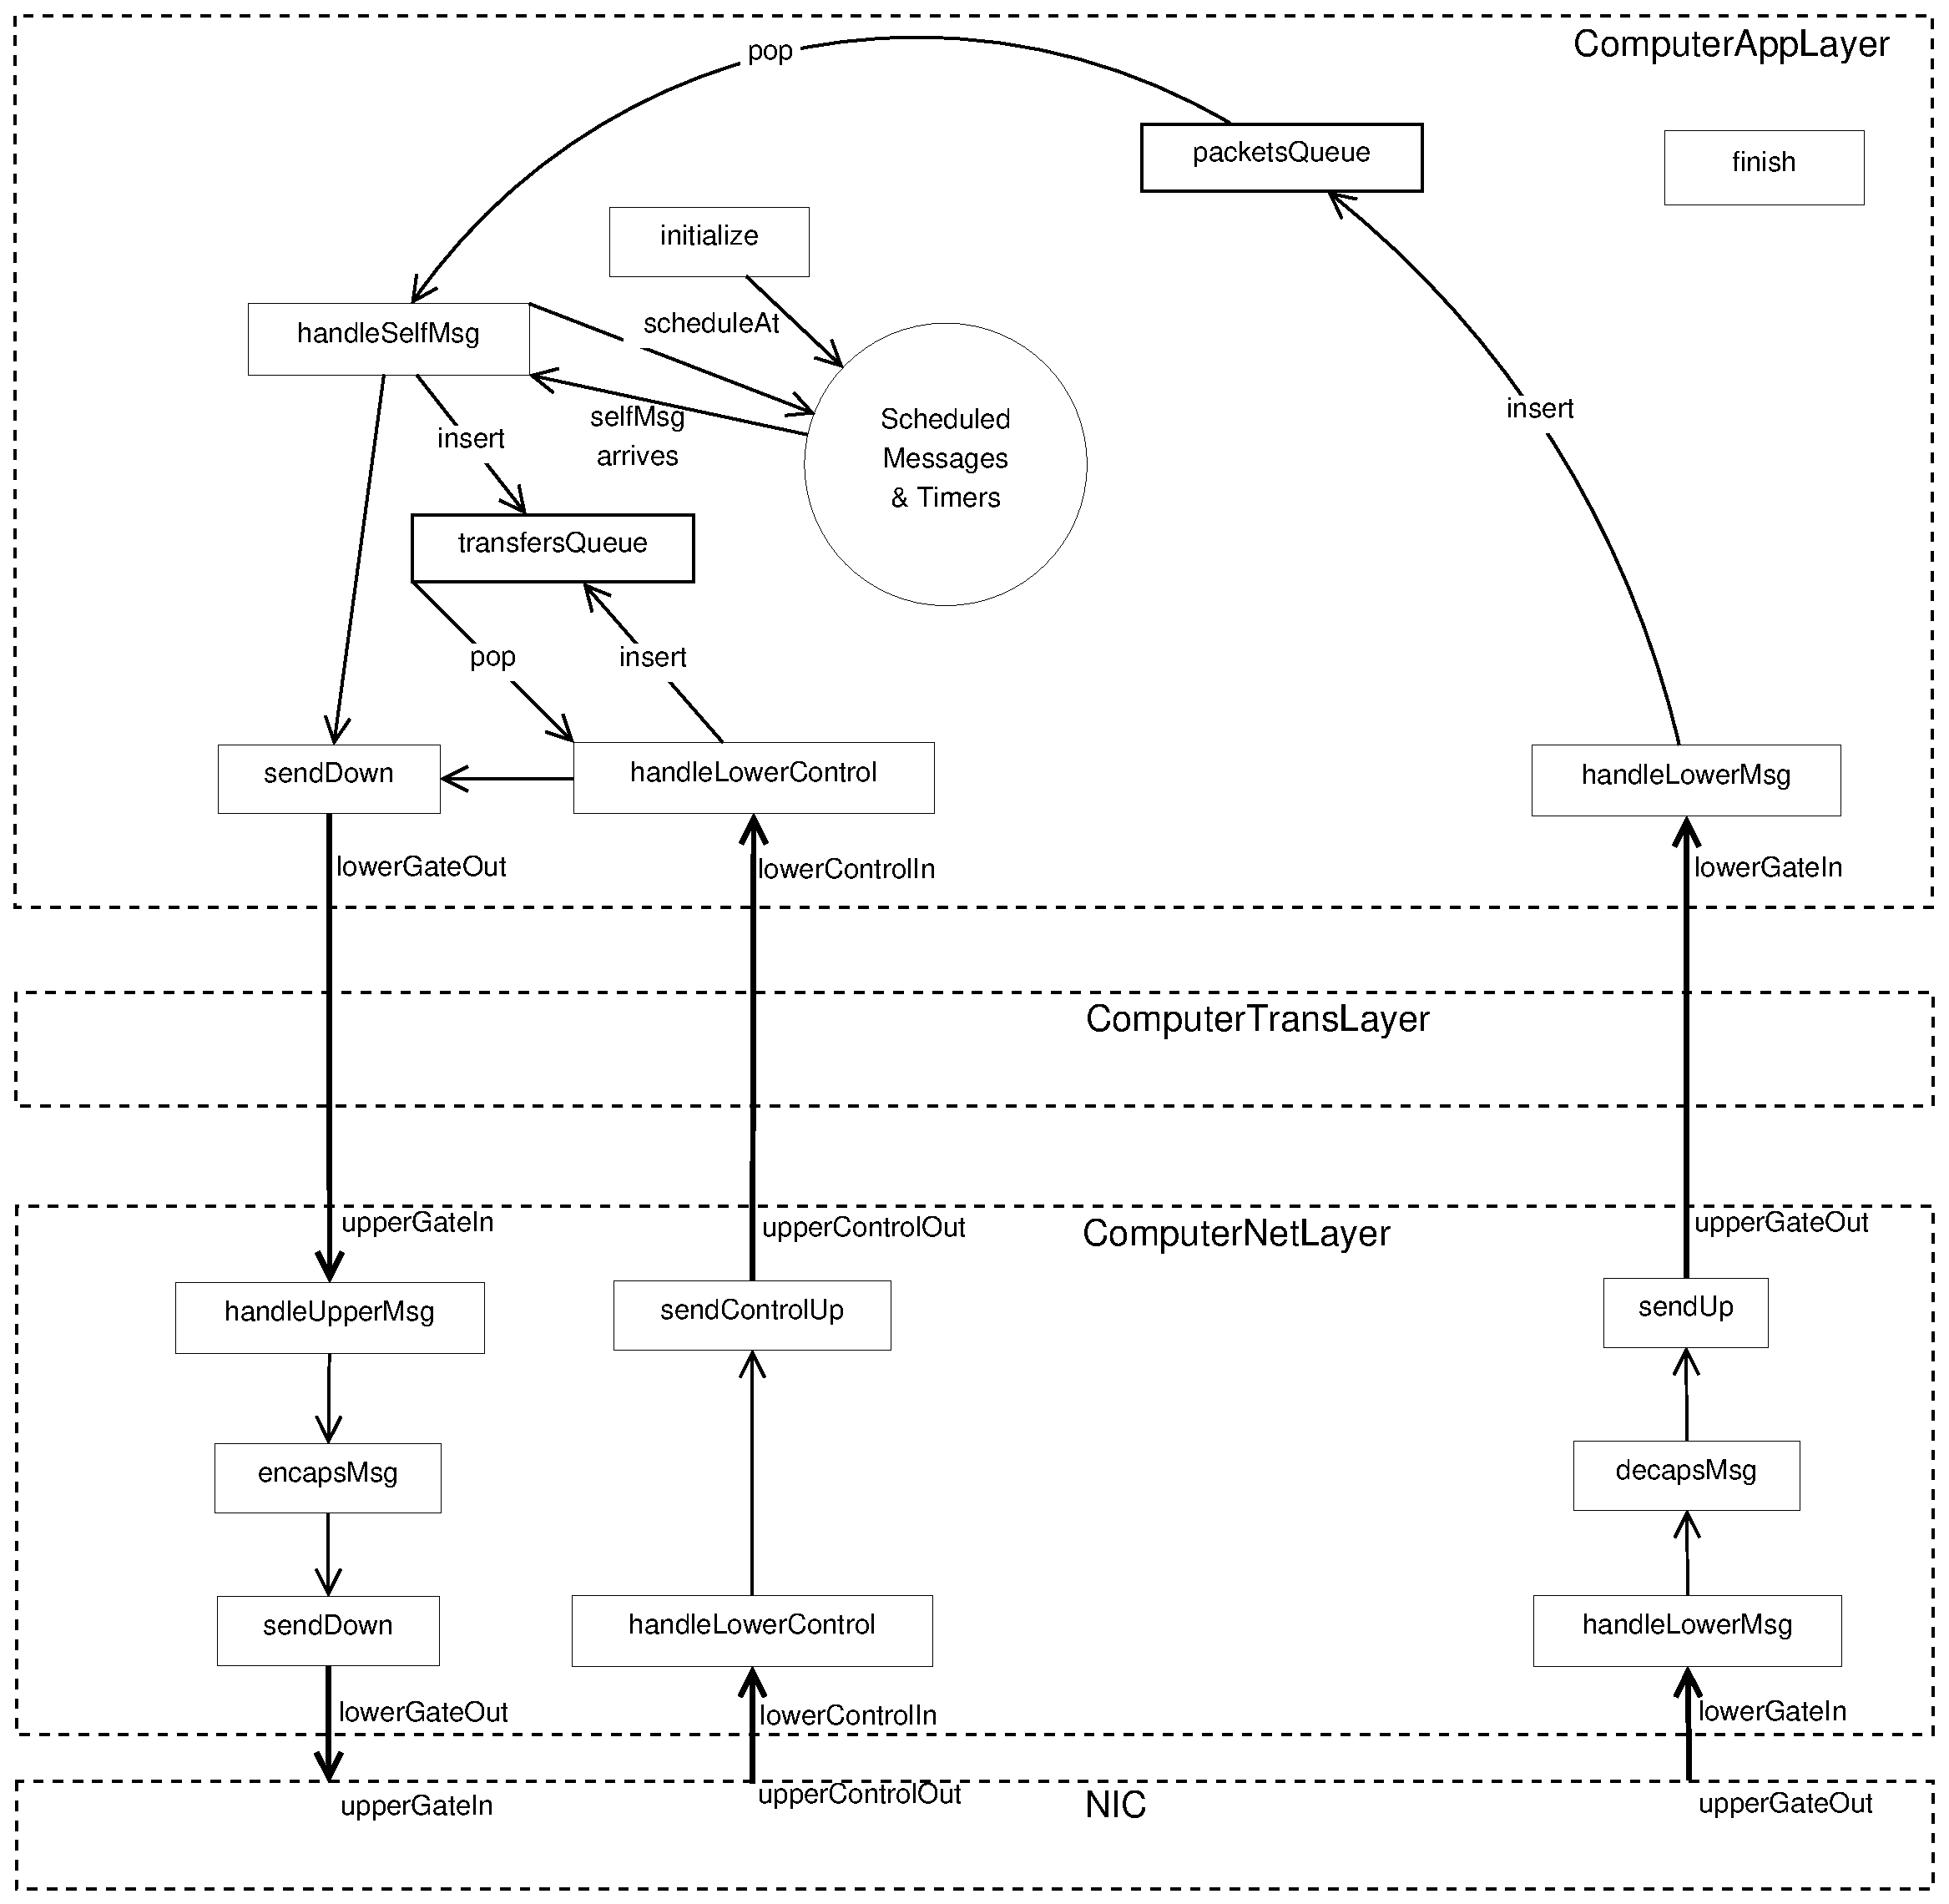
\includegraphics[width=0.9\textwidth]{Computerschema.eps}
 \end{center}
 \caption{Computer functionality diagram}
 \label{fig:Computerschema}
\end{figure}

All methods and elements in the figure will be described next:

\begin{itemize}
 \item \textbf{Scheduled Messages \& Timers}. This is like a big register where modules can store messages associated with a time. Whenever 
simulation time reaches one of this message's times, the message would be recovered from the register and received as self message in the 
module. Usually this message is handled by \textit{handleSelfMsg} method, which will filter the message according to its kind to decide
which action should be done. This register is used to program actions in a future time, send messages with delay or just to have timers
for any other use. To schedule a new message, the method \textit{scheduleAt} has to be used.
 
 \item \textbf{\textit{initialize}}. In this method, apart from initializing some variables, Computer calculates the slot distribution among the 
\acp{AN}. Slot calculation is done according to the algorithm showed in Section \ref{subsec:slottedsyncphase} (\nameref{subsec:slottedsyncphase}),
and it is done at \textit{stage} 3. At \textit{stage} 4 the length of the different phases in the period is calculated and the begin of the first
Sync Phase of the first period is scheduled to make the protocol start working.

 \item \textbf{\textit{finish}}. Records the number of dropped and erased packets due to different reasons, as well as the number of packets
correctly received and sent. It is executed at the end of the simulation.

 \item \textbf{\textit{sendDown}}. This method sends application packets to the \ac{MAC} going through the Transport and Network layers.

 \item \textbf{\textit{transfersQueue}}. This queue was created to store in Application Layer an exact copy of the \ac{MAC} queue. Whenever a packet
is sent down, a copy is stored in the \textit{transfersQueue}. This way, the packet trying to be sent by \ac{MAC} Layer, will be always on the
first position of the queue. In case the transmission fails or succeeds this will be notified from \ac{MAC} to Application Layer. Method
\textit{handleLowerControl} will handle this control message acting over the first position in \textit{transfersQueue} (will be explained later).

 \item \textbf{\textit{packetsQueue}}. Computer can receive only packets from \acp{AN} and never directly from \acp{MN}. The phases where \acp{AN}
and Computer communicate between them are ComSink 1 and 2. During ComSink Phase 1, the traffic goes direction computer (up-links), and during
ComSink Phase 2 the traffic goes direction selected \acp{AN} (down-links). This means that during ComSink 1, the Computer only receives messages
and during ComSink 2, it only sends messages. Therefore, a queue is needed to store all messages received during ComSink 1 until they are
transmitted during ComSink 2. This queue is the \textit{packetsQueue}.

 \item \textbf{\textit{handleLowerControl}}. When \ac{MAC} Layer wants to communicate to the Application Layer that some event occurred, it can do 
it using control messages. Possible control messages were commented in sub-section \ref{sec:macmodifications} (page \pageref{sec:macmodifications}),
and this method is the one in Application Layer in charge of handling them. Depending on the received control message, the following actions will
be done by the method:
  \begin{itemize}
    \item[-] \textit{PACKET\_DROPPED\_BACKOFF}. This control message is received when the transmitting packet in the \ac{MAC} Layer was dropped because
    the maximum number of Backoff tries in \ac{MAC} Layer was fulfilled (\textit{macMaxCSMABackoffs}). If this happens, the method extracts the first 
    message in \textit{transfersQueue} and increases the number of application retries due to Backoff for this message. If the maximum retries in 
    application is not yet reached, the message is transmitted again (and inserted into the queue), and if it is reached, the packet gets erased. 
    Dropped and erased packets are counted to be recorded with the \textit{finish} method.

    \item[-] \textit{PACKET\_DROPPED}. This control message is received when the transmitting packet in the \ac{MAC} Layer was dropped because
    the maximum number of retransmissions without receiving an \ac{ACK} was fulfilled. If this happens, the method extracts the first message in
    \textit{transfersQueue} and increases the number of application retries due to lack of \ac{ACK} for this message. If the maximum retries in
    application is not yet reached, the message is transmitted again (and inserted into the queue), and if it is reached, the packet gets erased.
    Dropped and erased packets are counted to be recorded with the \textit{finish} method.

    \item[-] \textit{QUEUE\_FULL}. This control message is received when the last packet sent down, found the \ac{MAC} Layer queue full. As 
    \ac{MAC} Layer queue is full, this layer cannot accept more packets and rejects it notifying to the Application Layer. If this happens, the message
    is removed from the \textit{transfersQueue} and a counter, indicating the number of packets erased due to \ac{MAC} Layer queue full, is increased.

    \item[-] \textit{SYNC\_SENT}. This control message is received when a broadcast was successfully transmitted into the channel. When this happens,
    , and to remain \textit{transfersQueue} like a copy of the \ac{MAC} Layer queue, the first element in \textit{transfersQueue} is deleted. This 
    value will be also recorded.

    \item[-] \textit{TX\_OVER}. This control message is received when a report was successfully sent and the \ac{ACK} was also received. When this 
    happens, for the same reason as before, the first element in \textit{transfersQueue} is deleted. This value will be also recorded.

    \item[-] \textit{ACK\_SENT}. This control message is received whenever an \ac{ACK} is sent by the \ac{MAC} Layer. For Computer or \ac{AN} cases 
    is not important, but it will be commented later in \ac{MN} explanation why is this control message needed.
  \end{itemize}


 \item \textbf{\textit{handleLowerMsg}}.

 \item \textbf{\textit{handleSelfMsg}}.


\end{itemize}


\subsection{\acp{AN} Application Layer}

\acp{AN} Application Layer functionality is contained in the class \textit{AnchorAppLayer}. The diagram in Figure \ref{fig:ANschema} 
shows a general overview of this Layer functionality together with the Network Layer. This class inherits from \textit{AppLayer} class, like
\textit{ComputerAppLayer} did.

\begin{figure}[ht]
 \begin{center}
  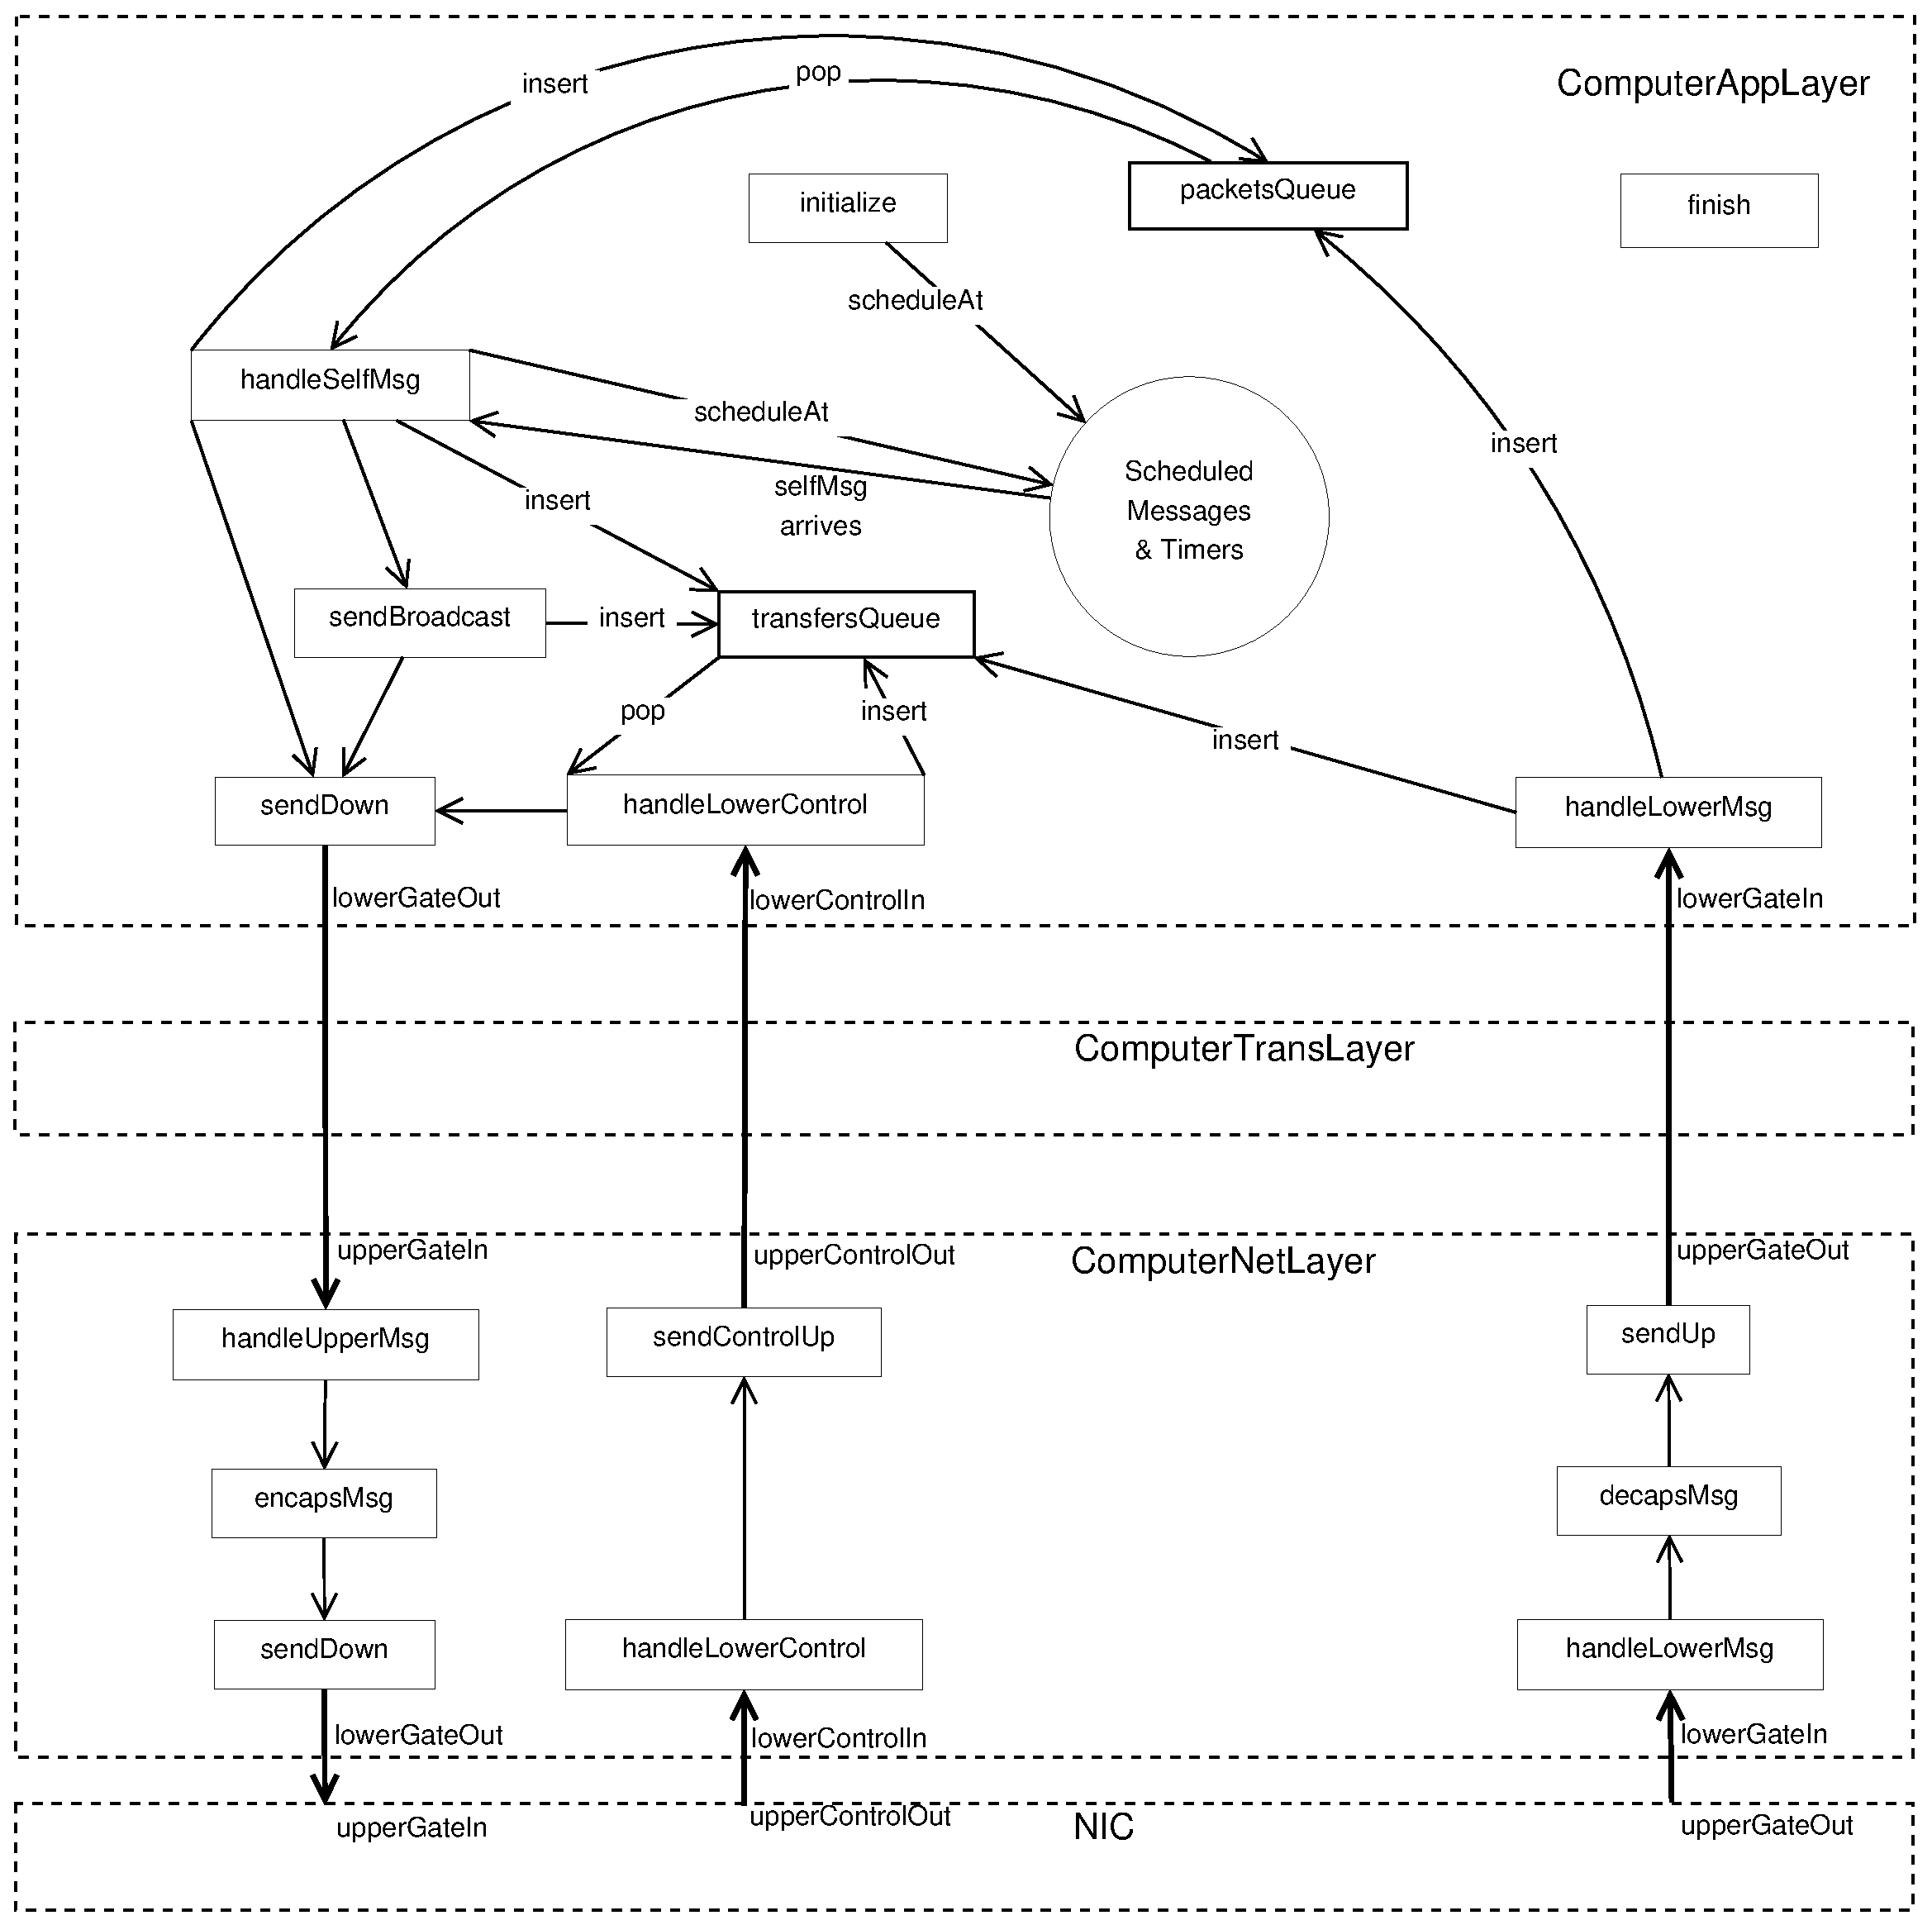
\includegraphics[width=0.9\textwidth]{ANschema.eps}
 \end{center}
 \caption{\acp{AN} functionality diagram}
 \label{fig:ANschema}
\end{figure}

All methods and elements in the figure will be described next:

\begin{itemize}
 \item \textbf{Scheduled Messages \& Timers}. This module for the \acp{AN}, works exactly the same as for the Computer. For a deeper explanation, check
the Computer Application Layer.

 \item \textbf{\textit{initialize}}. In this method, apart from initializing some variables, \acp{AN} schedule at \textit{stage} 4 the begin of 
the first Sync Phase of the first period to make the protocol start working.

 \item \textbf{\textit{finish}}. Records the number of dropped and erased packets due to different reasons, as well as the number of packets
correctly received and sent. It is executed at the end of the simulation.

 \item \textbf{\textit{sendDown}}. This method sends application packets to the \ac{MAC} going through the Transport and Network layers.

 \item \textbf{\textit{sendBroadcast}}. This method is called whenever a broadcast wants to be sent, for example during Sync Phase. Before sending
the message down, an application message is created and initialized with the correct message type and data. One thing to take into account is that
if the broadcast is a sync message, \ac{CSMA/CA} must be disabled and this is marked in the packet during this method. Remember that a copy must 
be inserted into the \textit{transfersQueue}.

 \item \textbf{\textit{transfersQueue}}. This module for the \acp{AN}, works exactly the same as for the Computer. For a deeper explanation, check
the Computer Application Layer.

 \item \textbf{\textit{packetsQueue}}. When an \ac{AN} receives a packet from another \ac{AN}, it must be during the ComSink Phases and for 
routing. This packet is immediately routed. When an \ac{AN} receives a packet (report or broadcast) from a \ac{MN}, it is during the
Report or \ac{VIP} Phases. If this packet is intended to be routed till the Computer (centralized mode), it has to be stored in a queue until
it can be sent during the next ComSink Phase 1. This queue is the \textit{packetsQueue}. All this process will be explained better in the 
following method explanations.

 \item \textbf{\textit{handleLowerControl}}. This method works exactly the same as for the Computer. For a deeper explanation, check the Computer 
Application Layer.

 \item \textbf{\textit{handleLowerMsg}}.

 \item \textbf{\textit{handleSelfMsg}}.

\end{itemize}


\subsection{\acp{MN} Application Layer}

\acp{MN} Application Layer functionality is contained in the class \textit{NodeAppLayer}. The diagram in Figure \ref{fig:MNschema} 
shows a general overview of this Layer functionality together with the Network Layer. This class inherits from \textit{AppLayer} class, like
\textit{ComputerAppLayer} did.

\begin{figure}[ht]
 \begin{center}
  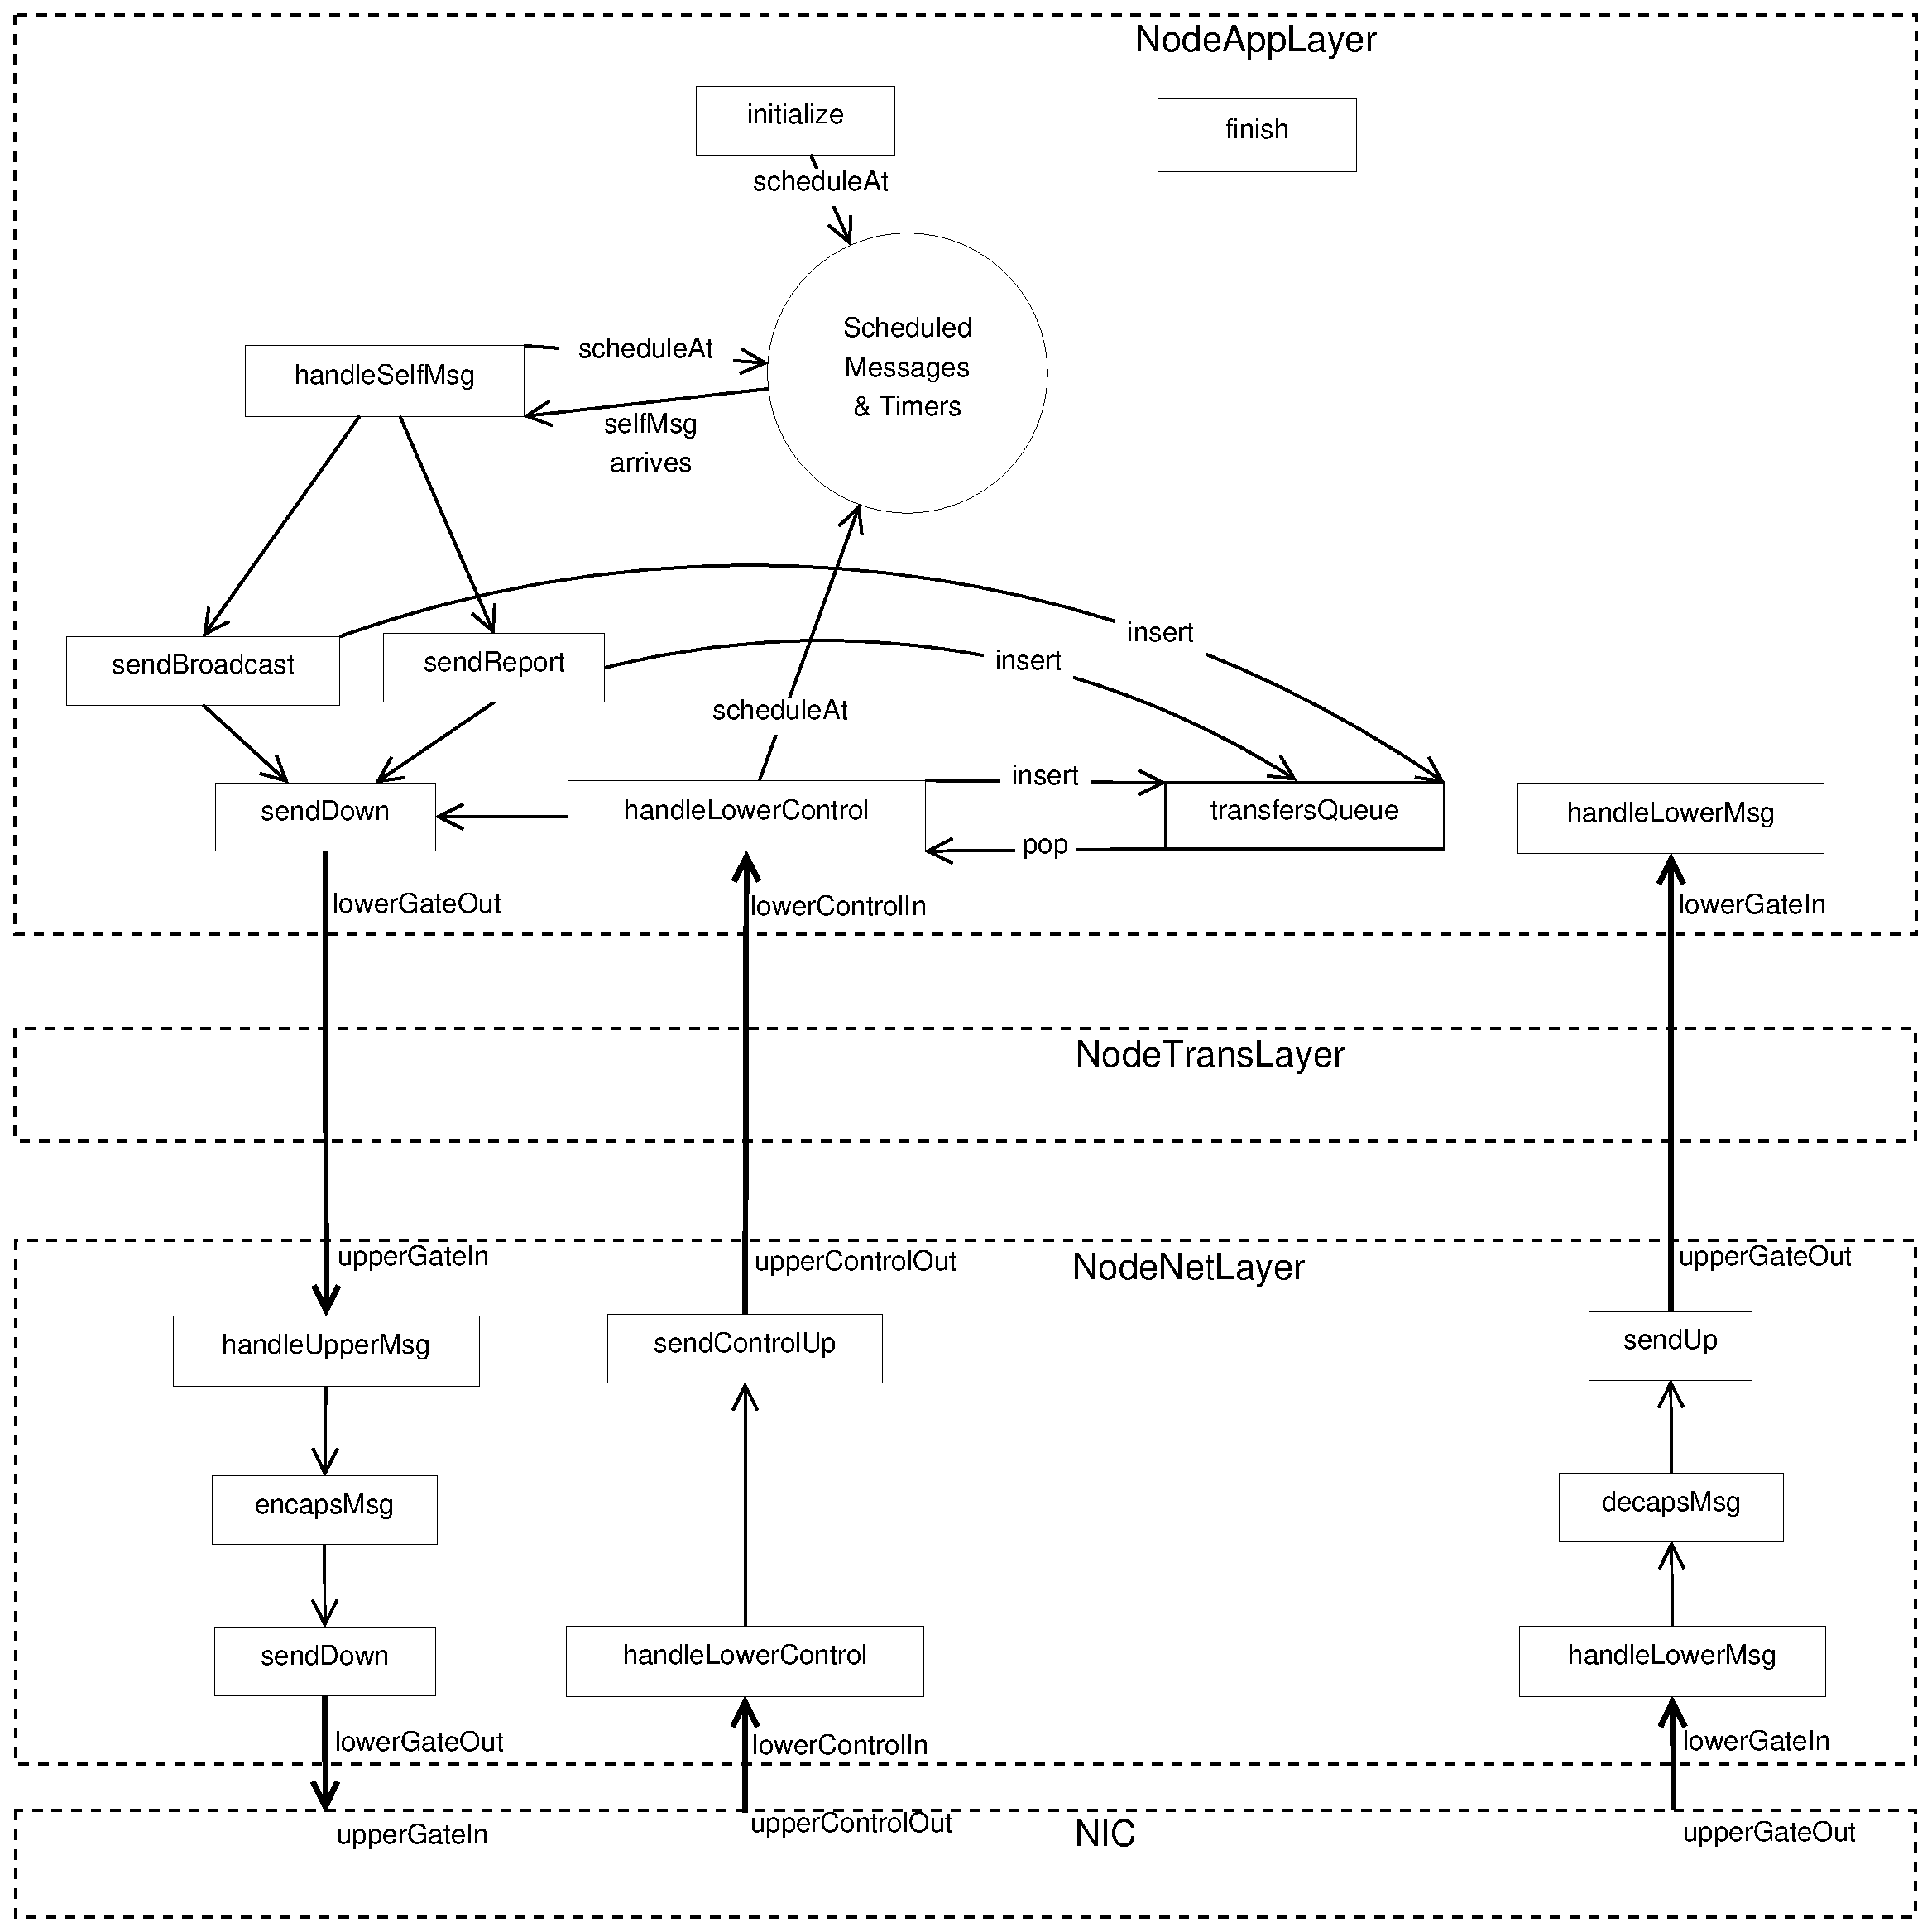
\includegraphics[width=0.9\textwidth]{MNschema.eps}
 \end{center}
 \caption{\acp{MN} functionality diagram}
 \label{fig:MNschema}
\end{figure}

All methods and elements in the figure will be described next:

\begin{itemize}
 \item \textbf{Scheduled Messages \& Timers}. This module for the \acp{MN}, works exactly the same as for the Computer. For a deeper explanation, check
the Computer Application Layer.

 \item \textbf{\textit{initialize}}. In this method, apart from initializing some variables, \acp{MN} schedule at \textit{stage} 4 the begin of 
the first Sync Phase of the first period to make the protocol start working.

 \item \textbf{\textit{finish}}. Records the number of dropped and erased packets due to different reasons, as well as the number of packets
correctly received and sent. It is executed at the end of the simulation.

 \item \textbf{\textit{sendDown}}. This method sends application packets to the \ac{MAC} going through the Transport and Network layers.

 \item \textbf{\textit{sendBroadcast}}. This method is called whenever a broadcast wants to be sent, during Report or \ac{VIP} Phases. Before 
sending the message down, an application message is created and initialized with the correct message type and data. Unlike for the \acp{AN},
here \ac{CSMA/CA} must remain active. Remember that a copy must be inserted into the \textit{transfersQueue}.

 \item \textbf{\textit{sendReport}}. \ac{MN}'s reports are just sent to selected \acp{AN}, that is why before sending them, it is always needed
to listen to any Sync Phase to find which \ac{AN} is our selected \ac{AN}. From the packets listened to, it is created a \ac{RSSI} list, which 
is the first thing \textit{sendReport} method checks to assign the destination address. In the case the \ac{RSSI} list does not exists, an 
error will notify about this fact. After assigning the destination address, real destination address is assigned. This address will be 
the Computer's address if the \ac{MN} is working in centralized mode and the selected \ac{AN} address in the case the \ac{MN} is working in 
Distributed-A mode.

Next thing to do is assign the packet size to model the real packet behavior. Depending on the type of report to be sent, different sizes will 
be chosen. A complete list of this types was already explained in sub-section \ref{sec:packetstructure} (page \pageref{sec:packetstructure}).

A last detail must be taken into account before sending the packet down. For the case where the packet asks for some information, the ASK flag
will be activated and the address of the selected \ac{AN} saved. This address is saved because, in case the \ac{MN} moves and its selected \ac{AN}
changes, the \ac{MN} will still need to ask for the information to the first \ac{AN}. This will be the \ac{AN} having the information ready to be 
requested, and not the new selected \ac{AN}. For the case where the packet requests for the previously asked information, the Request flag will
be activated. As it was said, the destination address to be used in this case, is the one saved by the \ac{MN} when asking for information.

Now the packet is ready to be sent down, but saving a copy before in the \textit{transfersQueue}.


 \item \textbf{\textit{transfersQueue}}. This module for the \acp{MN}, works exactly the same as for the Computer. For a deeper explanation, check
the Computer Application Layer.

 \item \textbf{\textit{handleLowerControl}}. The main functionality of this method is exactly the same as for the Computer. For a deeper explanation, 
check the Computer Application Layer. The difference between this method and the one for the Computer is that this method handles in which situations,
when receiving a control message, the \ac{MN} can go to sleep or must remain awake. All this cases will be explained later together with the ones from
the other methods.

 \item \textbf{\textit{handleLowerMsg}}. Whenever a \ac{MN} receives a packet in its Application Layer, this method is executed. The purpose
of this method is handling the different arrived packets according to the phase when they arrived. The following cases are possible:
\begin{itemize}
  \item Broadcasts arrived during any Sync Phase. This are the sync messages that \acp{MN} listen to get \ac{RSSI} samples and get 
  synchronized. This method makes a list with all \ac{RSSI} values per \ac{AN}. This list will be used by the \textit{sendReport} method to 
  decide which \ac{AN} is the selected \ac{AN}.

  \item Report from selected \ac{AN} answering a request, received during Report Phase. If a report answering a previous request comes, and 
  it comes during the waiting time left for this purpose, the answer will be considered as valid and the waiting time timer will get canceled to 
  avoid idle listening.
\end{itemize}

 \item \textbf{\textit{handleSelfMsg}}. Whenever a self message is received, it is handled by this method. The following kinds of self messages
are processed by this method:
 \begin{itemize}
  \item \textit{SLEEP}. It will be explained at the end of this section.

  \item \textit{WAKE\_UP}. It will be explained at the end of this section.

  \item \textit{SEND\_REPORT\_WITH\_CSMA}. In this case, the method will check if the \ac{MN} is already calculating its own position (\acp{MN} in
  Mode 2). When this is the case, the self message will be rescheduled a random time after the calculation process. If the \ac{MN} was not busy, 
  \textit{sendReport} method will be called.

  \item \textit{SEND\_SYNC\_TIMER\_WITH\_CSMA}. In this case, \textit{sendBroadcast} method is called to send a broadcast. If there are still 
  more broadcasts to send, the self message is rescheduled a time after. The times where the broadcasts are going to be sent are calculated by the
  method \textit{createRandomBroadcastTimes}.

  \item \textit{CALCULATE\_POSITION}. When this self message is received, there are two options. If the \ac{MN} was calculating its position, then
  the timer is ended and the energy status updated. If the \ac{MN} was not still calculating its position, a new timer is started scheduling its end
  some time after. This time will be the processing time. The \ac{MN}'s position is also stored in a list.

  \item \textit{WAITING\_REQUEST}. When a request is correctly transmitted, method \textit{handleLowerControl} starts a waiting time timer. When the
  self message due to this timer is received, means that no \ac{AN}'s answer was received on time. This method restarts then all waiting time 
  variables to its default values, and records this situation.

  Another situation where this kind of self message can arrive is when requesting information. When a \ac{MN} wants to perform a request, it 
  schedules a WAITING\_REQUEST self message at the middle of Sync Phase 1. It is made this way because in the middle of this phase all reports and 
  extra reports are already scheduled. When this self message is handled, the first thing to do is looking for a report or extra report where the 
  request flag could be activated. In case no report could be reused, a new one is scheduled.

  The request packet is one of the most important packets to be sent, and not losing it is a priority. That is why when a request is made from a 
  \ac{MN} in Mode 4, its broadcasts are canceled to reduce the traffic in the Report Phase, and hence arise the probability of a successfully 
  delivery.

  \item \textit{BEGIN\_PHASE}. This self message is scheduled during all the simulation at the beginning of every phase to configure it. The 
  first thing the method does when receiving a self message of this type, is deleting all messages in the \textit{transfersQueue} which did not 
  have time to be transmitted during the previous phase (the same is done in \ac{MAC} queue). After that, next thing to do is calculate next phase 
  start time, and reschedule the self message at that time. The following actions will be different depending on the phase:
  \begin{enumerate}
    \item \textit{SYNC\_PHASE\_1}. When this phase starts, and the period is active, the whole period will be configured. At this moment, the 
    following things are going to be done:
    \begin{itemize}
      \item Sync Phases to be listened are going to be enabled. It depends on the Sync Phase Offset, if the active period is the last one and
      if the \acp{MN} are in Mode 3.
      \item Clean \ac{RSSI} list before reading new Sync messages.
      \item Report for \acp{MN} in Modes 1 and 4 are going to be scheduled if the active period is the last one of the collection.
      \item If \ac{MN} is in Mode 2 and the active period is the last one of the collection, the timer for calculating the \ac{MN}'s position will 
      be started.
      \item Broadcasts random times are going to be calculated for \acp{MN} in Modes 3 and 4. The first broadcast is also going to be scheduled. 
      If there is an extra report in the period and \ac{MN} is in Mode 3, broadcasts are going to be canceled to save battery. A minimum time among
      broadcasts and with the reports should be left.
      \item If an extra reports is going to be scheduled in this period (depends on the configuration parameters), Sync Phase 1 must be enabled if it
      was not already. Before scheduling a new extra report, it has to be checked if another report is already scheduled. If this happens, the extra
      report will not be scheduled and the normal report will be used. Every time an extra report is processed, a counter is increased. When this
      counter reaches the value of the parameter \textit{askFrequency}, the extra report gets the ASK flag activated and the request packet is 
      scheduled for the next period.
    \end{itemize}




    \item \textit{REPORT\_PHASE}.
    \item \textit{VIP\_PHASE}.
    \item \textit{SYNC\_PHASE\_2}.
    \item \textit{COM\_SINK\_PHASE\_1}.
    \item \textit{SYNC\_PHASE\_3}.
    \item \textit{COM\_SINK\_PHASE\_2}.

  \end{enumerate}


 \end{itemize}



\end{itemize}

A last detail and probably the most important for the \ac{MN} is, when are the nodes going to sleep and when should they wake up? This transitions
are done during the previously explained methods, but they will be explained all together here for a better understanding.

Transition between SLEEP state and any other takes some time (times can be seen in source code in class \textit{EnergyConsumption}). This is why,
before sleeping a node, it has to be checked if some other event. where the node must be awake. is coming sooner than the time needed to sleep and
wake up the node again (this time will be named as T). From this, it results that \ac{MN} can go to sleep in the following situations:

\begin{itemize}
 \item At the beginning of ComSink 1 and 2 (Done in \textit{handleSelfMsg} method).
 
 \item At the beginning of Sync Phases in any of the following cases (Done in \textit{handleSelfMsg} method):
    \begin{itemize}
      \item[-] Inactive periods.
      \item[-] First offset periods.
      \item[-] Second and third Sync Phases in last active period.
      \item[-] Sync Phases belonging to the Sync Phases offset.
      \item[-] If \ac{MN} is in Mode 3.
      \item[-] If there are no active periods.
    \end{itemize}
  The only exception to this, where \ac{MN} cannot go to sleep, is when an extra report is scheduled. In this case it does not matter if the 
  previous conditions are fulfilled, at the beginning of the first Sync Phase in this period, the \ac{MN} cannot sleep.

 \item At the beginning of \ac{VIP} Phase if next broadcast is scheduled in a time bigger than T (Done in \textit{handleSelfMsg} method).

 \item At the beginning of a Report Phase if all these conditions get fulfilled (Done in \textit{handleSelfMsg} method):
    \begin{itemize}
      \item[-] If next extra report comes after T.
      \item[-] If next report comes after T.
      \item[-] If next broadcast comes after T (just for \ac{MN} in Mode 4).
    \end{itemize}

  \item When a report was successfully sent, if the \textit{transfersQueue} has no elements and all these conditions get fulfilled (Done in 
  \textit{handleLowerControl} method):
    \begin{itemize}
      \item[-] If next broadcast comes after T (just for \ac{MN} in Mode 4).
      \item[-] If the report was not a request. In this case instead of sleeping the \ac{MN}, a timer to wait for the \ac{AN}'s answer is started.
    \end{itemize}

  \item When erasing a report due to maximum number of retries, if the \textit{transfersQueue} has no elements and if next broadcast (just for 
  \ac{MN} in Mode 4) comes after T (Done in \textit{handleLowerControl} method).

  \item When a broadcast was successfully sent into the channel, if the \textit{transfersQueue} has no elements and all these conditions get 
  fulfilled (Done in \textit{handleLowerControl} method):
    \begin{itemize}
      \item[-] If next broadcast comes after T.
      \item[-] If next report comes after T (just for \ac{MN} in Mode 4).
      \item[-] If Sync Phase 2 begins after T (just for \ac{MN} in Mode 3).
    \end{itemize}

  \item When erasing a broadcast due to maximum number of retries, if the \textit{transfersQueue} has no elements and all these conditions get
  fulfilled (Done in \textit{handleLowerControl} method):
    \begin{itemize}
      \item[-] If next broadcast comes after T.
      \item[-] If next report comes after T (just for \ac{MN} in Mode 4).
      \item[-] If Sync Phase 2 begins after T (just for \ac{MN} in Mode 3).
    \end{itemize}

  \item When waiting time in request process ended, if the \textit{transfersQueue} has no elements and if next broadcast (just for \ac{MN} in 
  Modes 3 and 4) comes after T (Done in \textit{handleSelfMsg} method).

  \item When an answer from an \ac{AN} to a request is received and the \ac{ACK} is sent, if the \textit{transfersQueue} has no elements and 
  if next broadcast (just for \ac{MN} in Modes 3 and 4) comes after T (Done in \textit{handleLowerControl} method).

\end{itemize}

Like for the previous case, transition times between SLEEP state and any other state are important. That is why, if the \ac{MN} must be awake for 
a certain event, it is important to wake it up some time before this event is coming. This time must be at least the time needed by \ac{MN} to go 
from SLEEP state to \ac{Rx} state (this time is named ``$T_2$''). \ac{MN} must wake up in the following situations:

\begin{itemize}
  \item A time $T_2$ before the start of each Sync Phase if all this conditions are fulfilled (Done in \textit{handleSelfMsg} method):
    \begin{itemize}
      \item[-] If \ac{MN} is not in Mode 3.
      \item[-] If the period is an active one.
      \item[-] If the Sync Phase is not affected by Sync Phase Offset.
      \item[-] If the Sync Phase is not the second or third Sync Phases in last active period.
    \end{itemize}
  
  \item A time $T_2$ before the start of Sync Phase 1 if there is an extra report scheduled in this period (Done in \textit{handleSelfMsg} method).
  
  \item A time $T_2$ before a report is going to be sent.

  \item A time $T_2$ before an extra report is going to be sent.

  \item A time $T_2$ before a broadcast is going to be sent.
\end{itemize}

It is important to remember that any time a report, extra report or broadcast gets canceled, the wake up order must be also canceled or the \ac{MN}
will wake up for nothing.

Both sleeping the \ac{MN} and waking it up actions, are called with the methods \textit{goToSleep} and \textit{goToWakeUp} respectively. Whenever
one of this two methods is called, it adds to an array a new time where the \ac{MN} should sleep or wake up. This arrays are then ordered to get
first the times coming sooner. When the arrays are already ordered, a self message is scheduled for each array's first element, at the indicated 
time. This self message will be handled by the \textit{handleSelfMsg} method. When this method receives a message to sleep or wake up the \ac{MN},
it does the following:
\begin{itemize}
 \item[-] Sleeps or wakes up the Radio changing its state to SLEEP or \ac{Rx}.
 
 \item[-] Updates the Energy module status calling the \textit{updateStateStatus} method from \textit{EnergyConsumption} class.

 \item[-] Removes the already handled time from the array.

 \item[-] Schedules the next time if there are still times to schedule.
\end{itemize}




\clearpage{\pagestyle{empty}\cleardoublepage}
\chapter{Simulation and Results}
\label{chap:simulationandresults}

In this chapter, different scenarios for the simulation and their results will be exposed and commented. To make it easier to understand, and as 
previously this two cases were also separated, first just the Sync Phase will be analyzed and then the whole protocol together.

In all the scenarios, simulations are independent among them and at least 100 repetitions are going to be done, this way the confidence intervals
shown in all figures could be calculated like in (\ref{mat:confidenceintervals}).

\begin{equation}
  x-\frac{\sigma}{\sqrt{n}}\cdot t_{\frac{\alpha}{2}} < \mu < x+\frac{\sigma}{\sqrt{n}}\cdot t_{\frac{\alpha}{2}}
  \label{mat:confidenceintervals}
\end{equation}

Where x is the value to check, $\sigma$ is the standard deviation of the measurements, $\mu$ is the average value, n is the number of repetitions done and 
$t_{\frac{\alpha}{2}}$ is a constant of 1.96 for a confidence interval of 95\%.

\section{Sync Phase simulation and analysis}

The aim of this section is to compare slotted transmission and random transmission during Sync Phase. This two approaches were already commented 
during Chapter \ref{chap:protocoldesign}: \nameref{chap:protocoldesign}.

As random transmission case is more difficult and chaotic as the slotted one, this will be studied separately first, leaving the slotted case to 
be studied together with the comparison and finishing with a study of the number of slots depending on the \acp{AN} density.

\subsection{Random Transmission}

To study this case, scenarios in Figure \ref{fig:hiddenvsnohidden} were simulated. In a) can be seen that all nodes can detect all node transmissions,
avoiding so Hidden Terminal Problem. In b), \acp{AN} can detect only some of the \ac{AN} transmissions and the \ac{MN} can detect all of them, this way
\acp{AN} are going to start transmitting when probably another \ac{AN} will be doing so, provoking a collision at the \ac{MN}. The number of \acp{AN}
is 6 in both cases and the number of \acp{MN} is 1.

\begin{figure}[ht]
 \begin{center}
  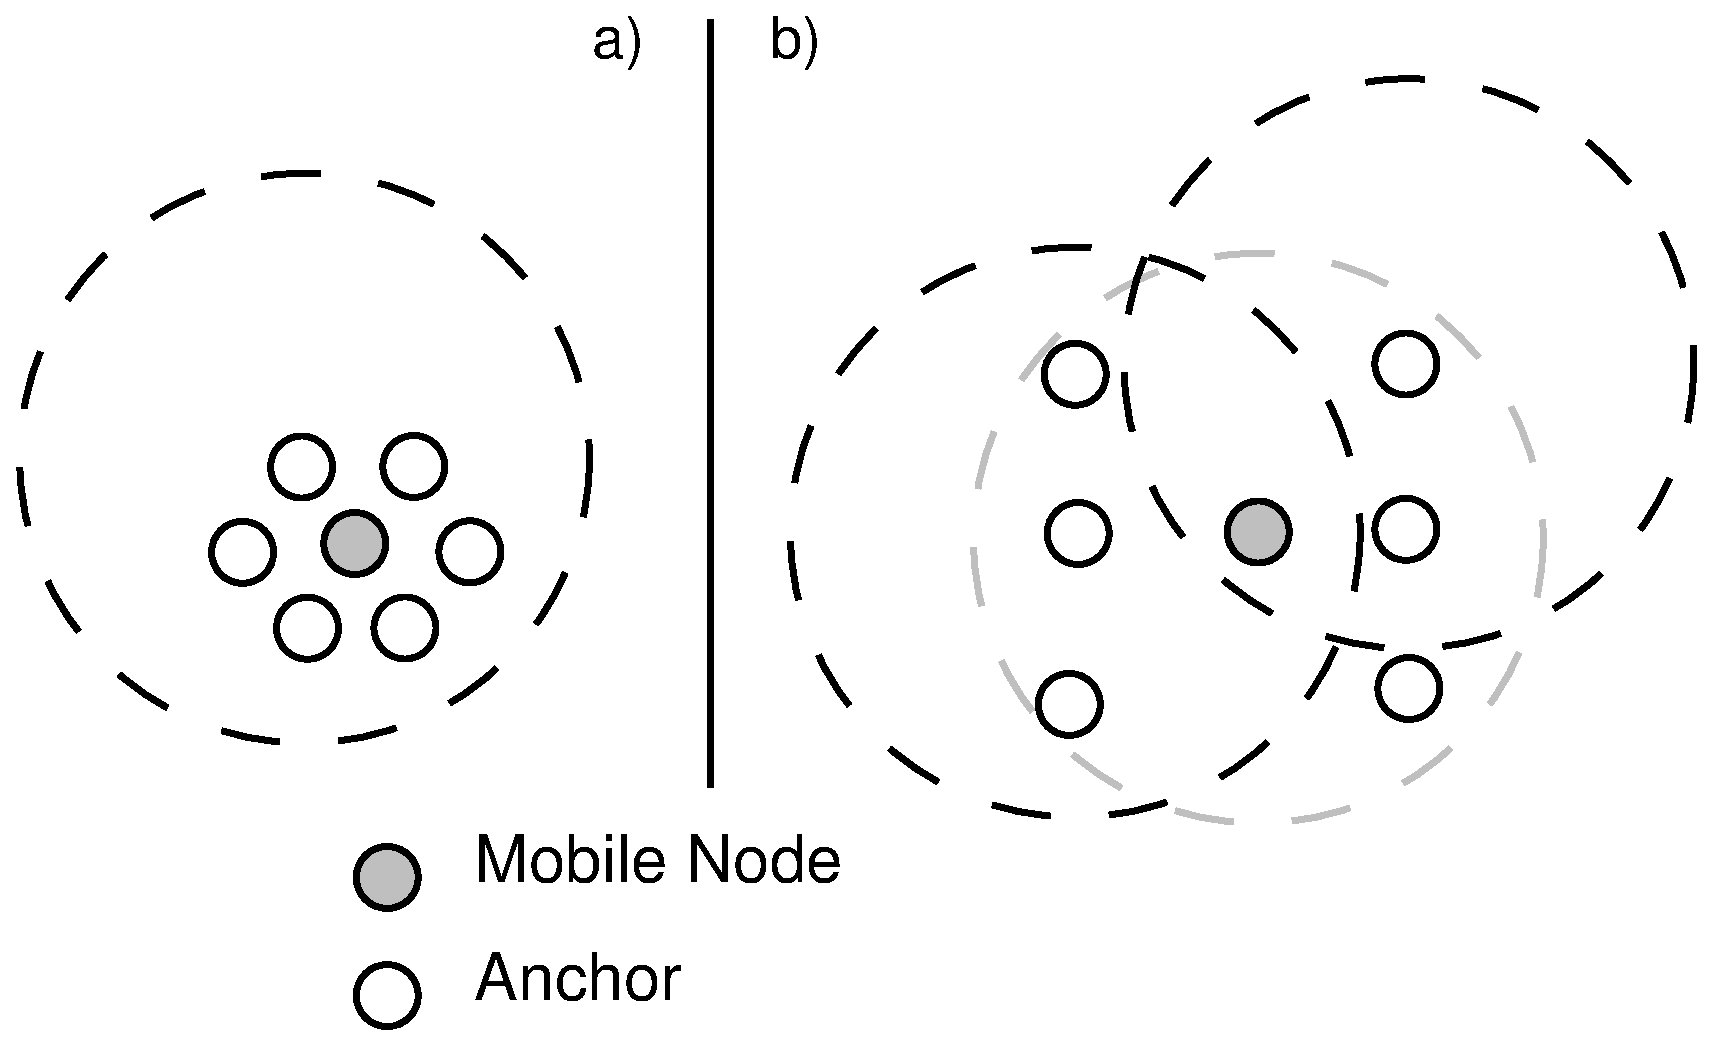
\includegraphics[width=0.5\textwidth]{hiddenvsnohidden.eps}
 \end{center}
 \caption{Scenarios avoiding (a) and forcing (b) Hidden Terminal Problem}
 \label{fig:hiddenvsnohidden}
\end{figure}

All errors caused by noise and random errors due to the channel, were disabled during this simulation. This is so, to have only simultaneous \acp{CCA} 
problem and Hidden Terminal Problem. With this situation, it can be assured that if a packet is received incorrectly in the \ac{MN}, the reason would 
be one of this two problems.

As is was commented in Chapter \ref{chap:protocoldesign}: \nameref{chap:protocoldesign}, in order to avoid an unknown random time during active 
synchronization, \ac{CSMA/CA} must be disabled. If this is done, all \acp{AN} will transmit at the same time generating lots of collisions. To solve this
a random time is added by Application Layer before the packet is transmitted. This random time value, will be between 0 and a maximum number. In this
section, this maximum number goes from 1 to 30 originating 30 different simulations. This value will be the X axis in all Figures. 

In order to reduce the dispersion caused by random numbers, each simulation will be done 1000 times.

\begin{figure}[ht]
 \begin{center}
  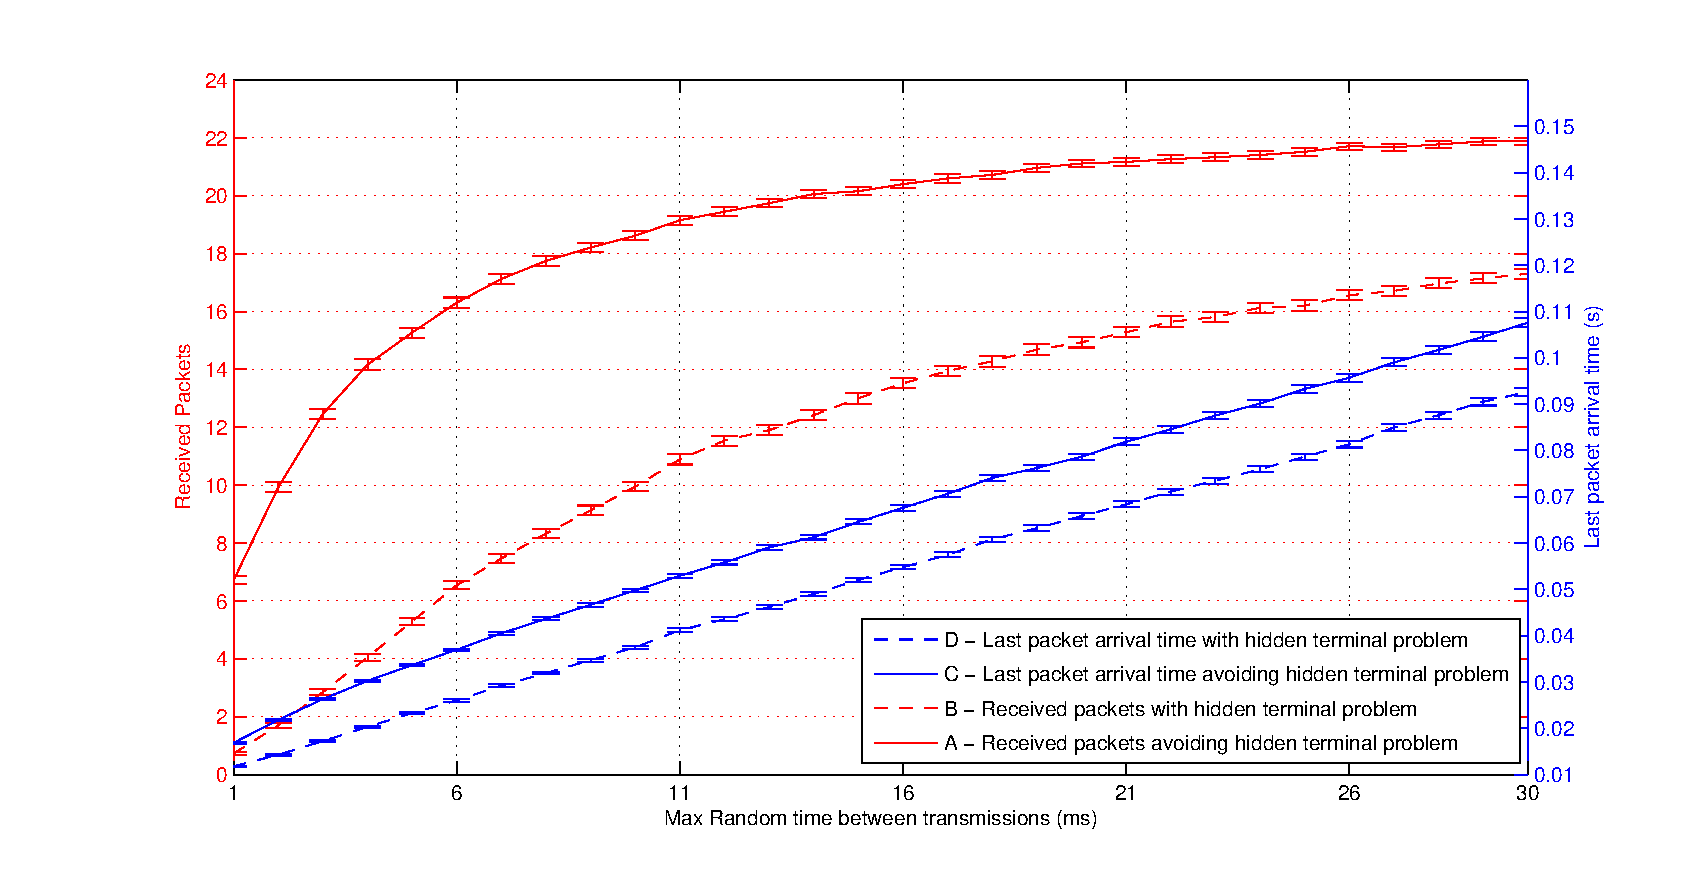
\includegraphics[width=1\textwidth]{receivedPacketsAndLastPacketArrival.eps}
 \end{center}
 \caption{Received packets in \ac{MN} and last packet arrival time}
 \label{fig:receivedPacketsAndLastPacketArrival}
\end{figure}


First simulation, gives as result \textbf{Figure \ref{fig:receivedPacketsAndLastPacketArrival}}. Here can be seen the total received packets in the 
\ac{MN} and the time when the last packet arrived in function of the maximum inter packet transmission time.

Both received packets lines (A and B) have a rising trajectory and both tend to 24 in the infinite. This 24 packets are the total number of 
packets sent to the network, sending each \ac{AN} four. It can be seen that, as in the case without Hidden Terminal Problem (A) the number of collisions
is smaller, the number of received packets in the \ac{MN} is much bigger than in the Hidden Terminal Problem case.

This Figure shows also the average arrival time from the last arrived packet in the \ac{MN}. This is not the 24$^{th}$ sent packet, as this could 
possibly collide with another. As the number of arrived packets in the case avoiding Hidden Terminal Problem is bigger, the last packet takes more time 
to arrive to the \ac{MN}. This can be seen in the Figure as C line values are always bigger than D line ones.

\begin{figure}[ht]
 \begin{center}
  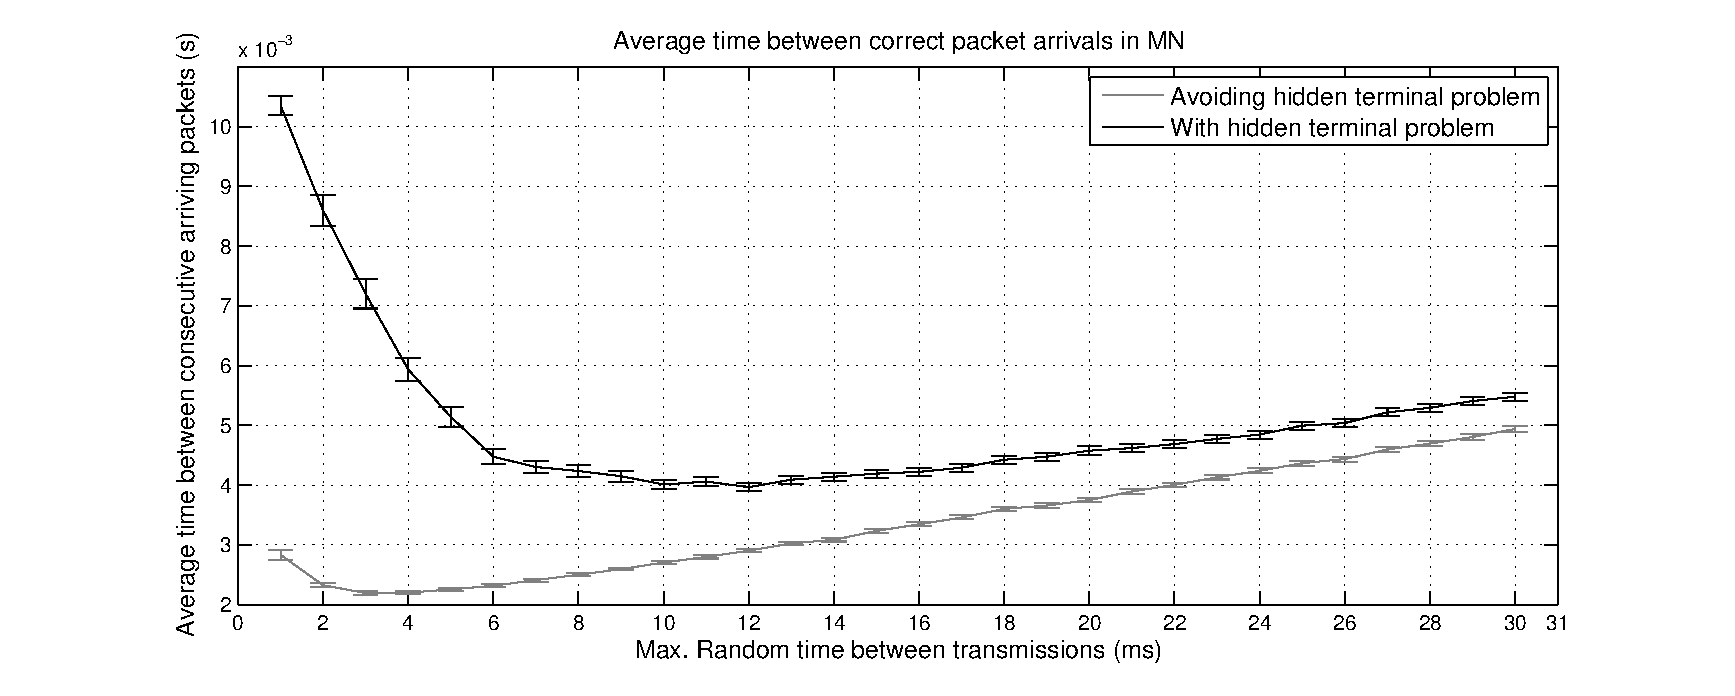
\includegraphics[width=1\textwidth]{averageTimeBetweenArrivals.eps}
 \end{center}
 \caption{Average time between arrivals in the \ac{MN}}
 \label{fig:averageTimeBetweenArrivals}
\end{figure}

\textbf{Figure \ref{fig:averageTimeBetweenArrivals}} shows the average times between packet arrivals in function of the maximum inter packet 
transmission time. This time does not represent the arrival time between two packets from the same \ac{AN}, but from any \ac{AN}. It is seen how
for the case with Hidden Terminal Problem, the time between consecutive arrived packets is much bigger than for the case without Hidden Terminal Problem,
consequently the number of collisions is also bigger, needing the \ac{MN} to wait more time until it gets another valid packet.

It is logic to think, that the bigger the time between transmissions, the bigger the time inter arrived packets. But, why in both cases, with or 
without Hidden Terminal Problem, for low values in X axis, the Y values start high and decrease until a certain moment where they start to grow again? 
This is because at the beginning, when the time between transmissions is low, the number of collisions is high as all \acp{AN} are trying to send their
packets almost at the same time. As the X value becomes bigger, the number of collisions gets reduced and thus the inter packet arrival time. But from 
the moment where the curves make their minimum, the influence of the time between transmissions becomes important, and makes the curves go up again.

\begin{figure}[ht]
 \begin{center}
  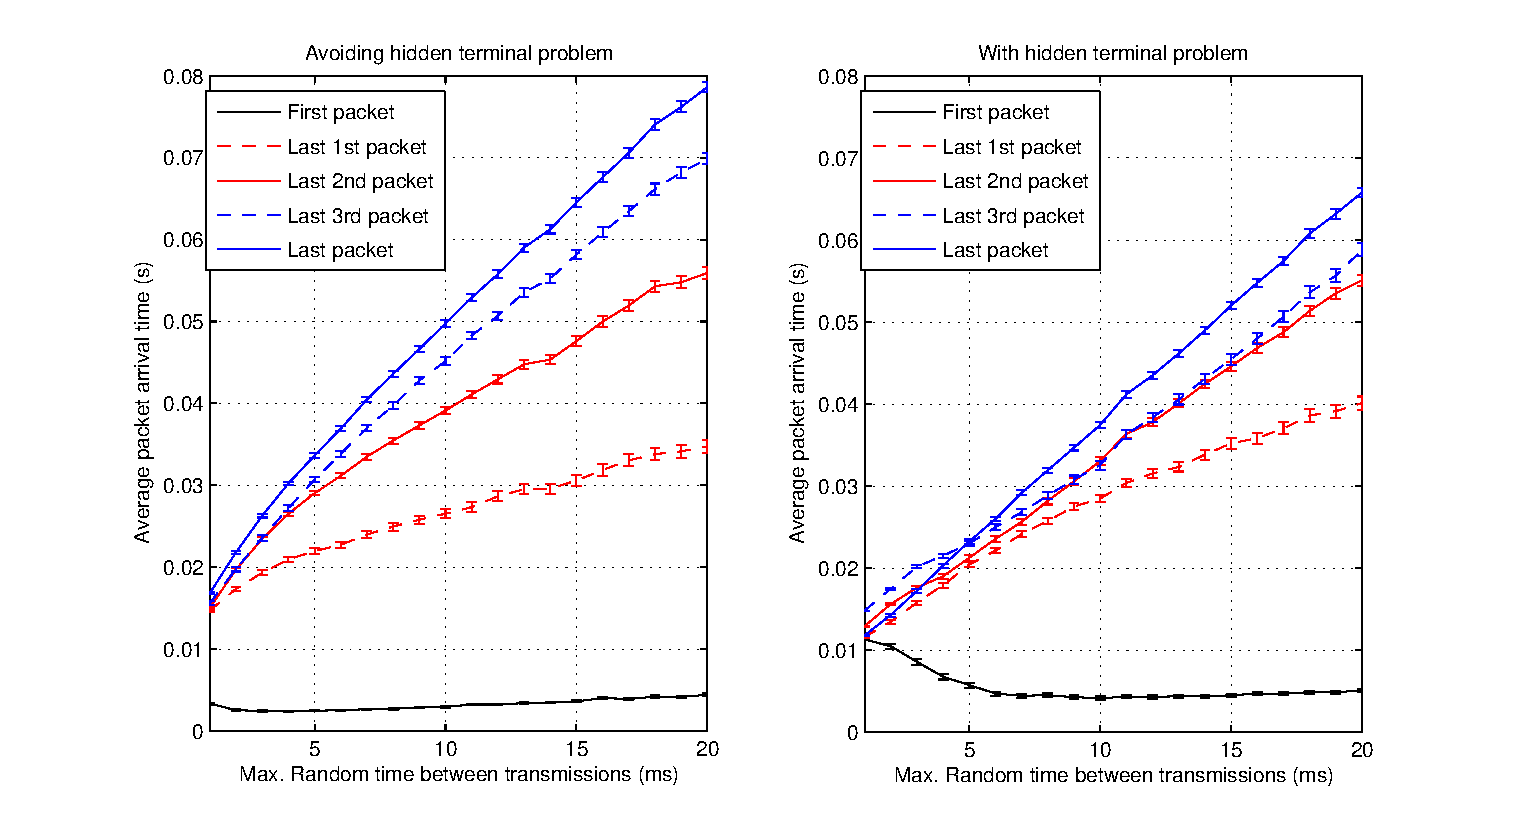
\includegraphics[width=1\textwidth]{averageDifferentTimes.eps}
 \end{center}
 \caption{Packet arrival average times}
 \label{fig:averageDifferentTimes}
\end{figure}

\textbf{Figure \ref{fig:averageDifferentTimes}} shows the average arrival time in the \ac{MN} of the first packet, the last first packet, the last
second packet, the last third packet and the last packet coming from any of the \acp{AN}.

It is easy to see that arrival time of the first packet should be smaller than the arrival time of the last first packet, this should be smaller than
 the arrival time of the last second packet, this should be smaller than last third and this smaller than the last. But if the case with Hidden 
Terminal Problem is observed, it can be found that when time between transmissions is small, last second and last third received packets arrive later 
that last received packet. How is this possible? This happens because due to the big number of collisions many times only first packets arrive or many of 
them arrive after the last second or third packets. When conditions are better (higher time between transmitted packets or no Hidden Terminal Problem) 
this does not happen because many more second or third packets are delivered and thus they will be the last packets.

It is also interesting how unlike the right figure, for the case without Hidden Terminal Problem, the arrival time of the first packet and the arrival 
time of the last first packet are quite separated. This is because in this case the collision number is much smaller, and as it was seen in Figure 
\ref{fig:receivedPacketsAndLastPacketArrival}, the \ac{MN} receives much more first packets from the \acp{AN}.

As comparison between the two cases, it can be seen that for the case without Hidden Terminal Problem, the arrival times are bigger, this is again because
the \ac{MN} receives in this case much more packets due to a lower number of collisions, making the last packets arrive later. This lower number of 
collisions makes also that the arrival time of the first packet is smaller than for the case with Hidden Terminal Problem.

\begin{figure}[ht]
 \begin{center}
  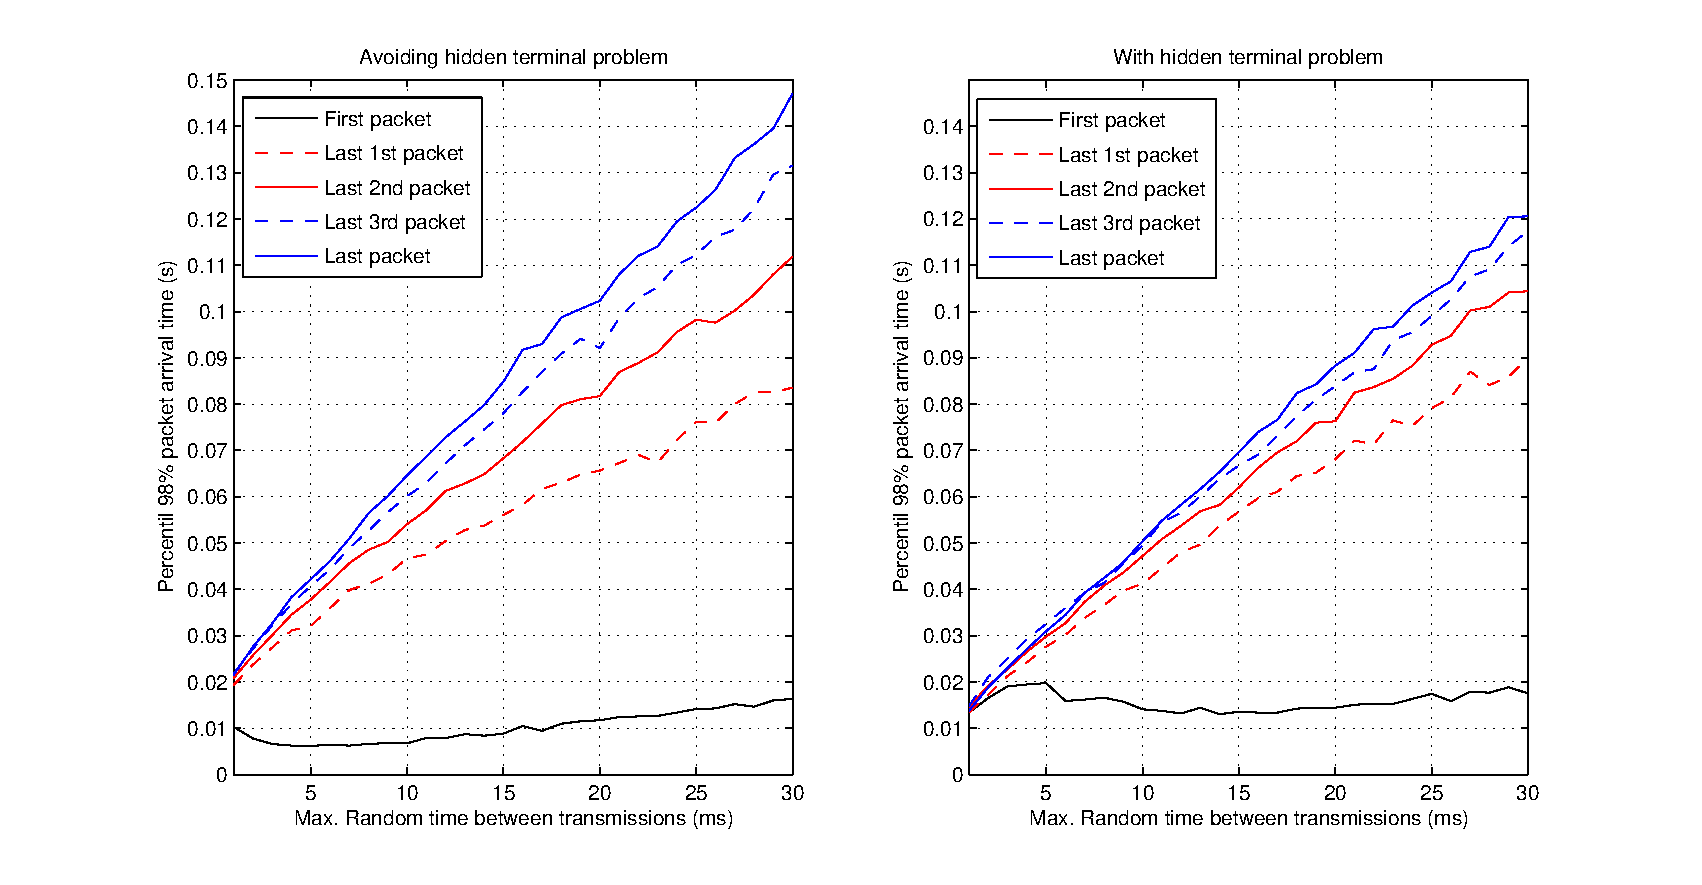
\includegraphics[width=1\textwidth]{percentil98differentTimes.eps}
 \end{center}
 \caption{Percentil 98 of packet arrival times}
 \label{fig:percentil98differentTimes}
\end{figure}

\textbf{Figure \ref{fig:percentil98differentTimes}} does not represent an average but a percentil 98, this means that if this times are taken as 
reference, in 98\% of the situations, the times are going to be under this values. This is thus a good way to get an acceptable top limit.

The analysis from this graphic is the same as the previous one with the only peculiarity that all times in Y axis are bigger, this is so because
this graphic represents the worst cases, not the average. For the same reason, in the case with Hidden Terminal Problem when the times between
transmissions are small, the first arrived packet time is bigger and behaves different as in Figure \ref{fig:averageDifferentTimes}.

\subsection{Slotted vs. Random Transmission}

The aim of this sub-section is to compare the random and the slotted transmission during the Sync Phase of the protocol. As slotted case seems to be
much better than random case, the first thing to make is looking for the best case in random transmission. To find this best case an optimum number
of broad-casted packets and time between transmissions should be found.

The scenario has 80 \acp{MN} uniformly and randomly distributed along the playground, and 30, 40, 50, 60 and 70 \acp{AN} distributed the same way.
There is hence Hidden Terminal Problem.

In order to reduce the dispersion caused by random numbers, each simulation will be done 100 times. Data will be measured in the \acp{MN}, and as 
they are disperse all over the playground, their values could be very different. That is why first an average of the 80 nodes will be done followed 
by an average of the 100 repetitions.

\subsubsection{Slot Number vs. \acp{AN} Number}

This sub-section's aim is checking how good is the algorithm to calculate the slot distribution among the \acp{AN}. For this purpose, an scenario 
with different number of \acp{AN} where slots will be calculated by a Computer as described in Chapter \ref{chap:protocoldesign}: 
\nameref{chap:protocoldesign}, will be simulated 100 times. It has to be taken into account that Computer takes also its own slot, this can be seen
like \acp{AN} number is one unit bigger.

The number of slots will be also useful for the following sub-sections, as to be able to compare randomly and slotted approaches, the Sync Phases need 
to last the same time, and this time cannot be known for random case until the number of slots is known.

\begin{figure}[ht]
 \begin{center}
  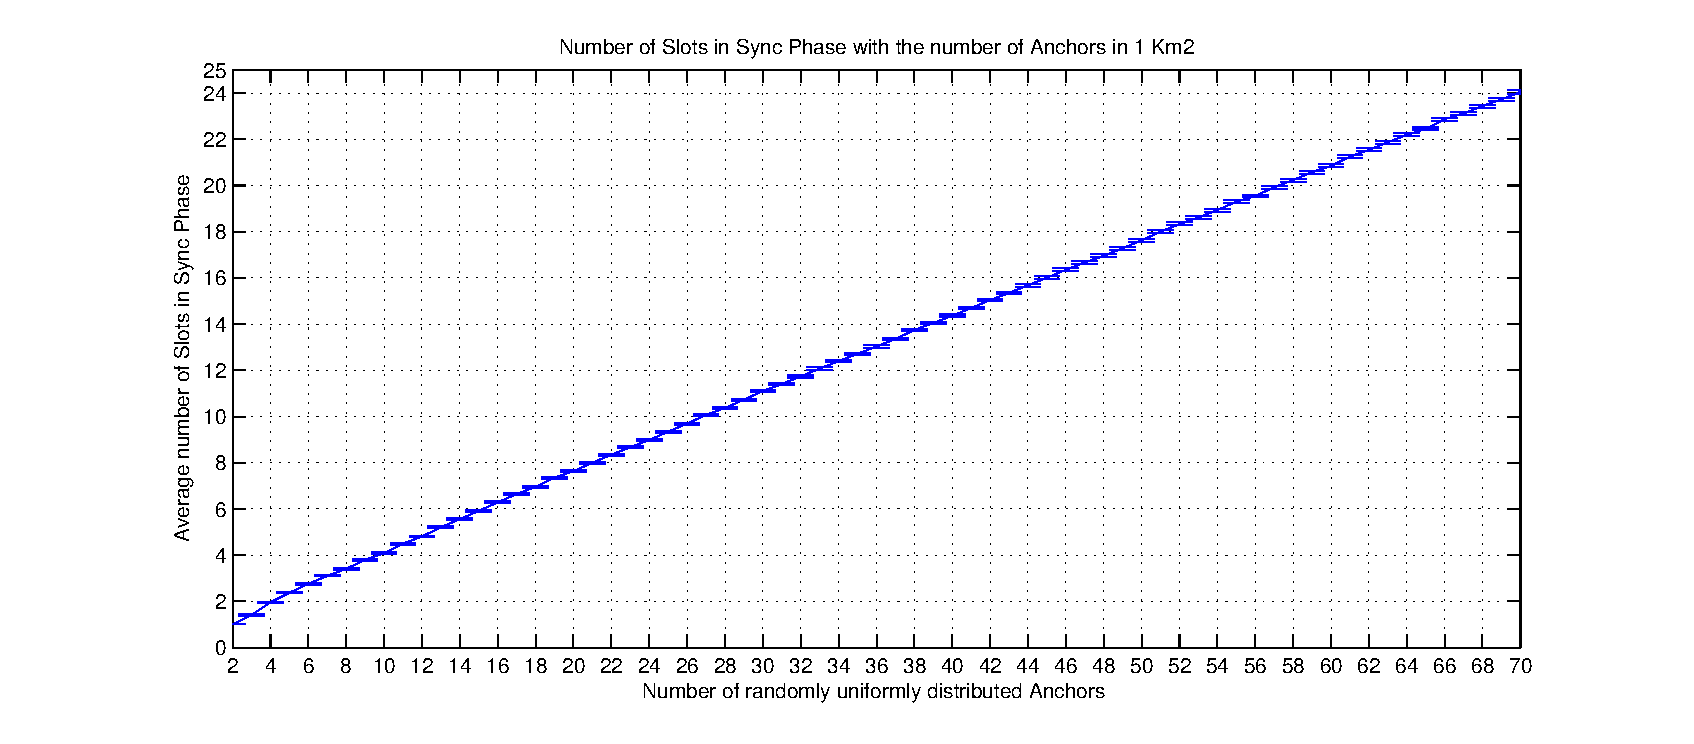
\includegraphics[width=0.8\textwidth]{numberOfSlotsWithTheAnchorDensity.eps}
 \end{center}
 \caption{Slot Number for a variable \acp{AN} density}
 \label{fig:numberOfSlotsWithTheAnchorDensity}
\end{figure}

\textbf{Figure \ref{fig:numberOfSlotsWithTheAnchorDensity}} is the result of simulating a 1 $Km^2$ playground with a number of \acp{AN} going from 
2 to 70, as the playground is fixed and only the number of nodes increase, it could be said that \acp{AN} density increases. When \acp{AN} density 
increases, and as \acp{AN} range stays constant, the number of neighbors for each \ac{AN} increases also. This makes the number of slots grow together
with the number of \acp{AN}, as it can be seen in the figure.

\begin{figure}[ht]
 \begin{center}
  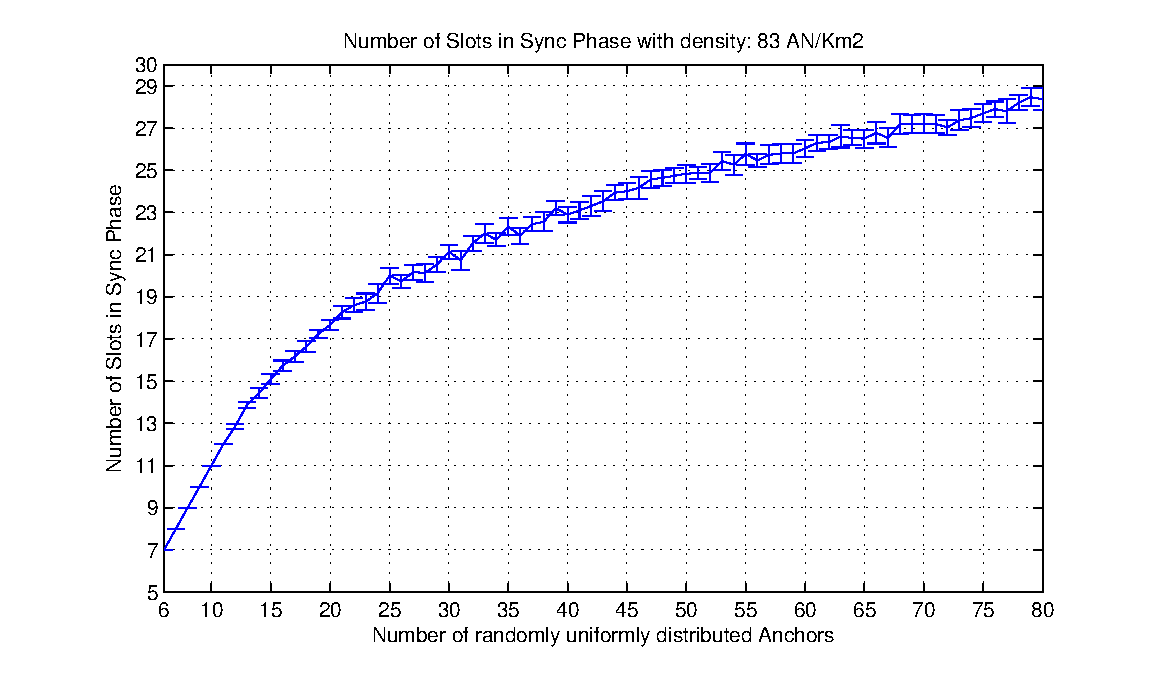
\includegraphics[width=0.8\textwidth]{numberOfSlotsWithTheSameDensity.eps}
 \end{center}
 \caption{Slot Number for a fixed \acp{AN} density}
 \label{fig:numberOfSlotsWithTheSameDensity}
\end{figure}

In this case, \textbf{Figure \ref{fig:numberOfSlotsWithTheSameDensity}} is obtained simulating 6 to 80 nodes with a minimum separation between them of 
80 meters. Playground is calculated dynamically with this parameters to have always a 83 $\acp{AN}/Km^2$ density. As \acp{AN} density remains constant,
the number of neighbors an \ac{AN} has also does. This means the re-usability of the slots will grow with the number of nodes. The re-usability can be
observed in the figure, as when the number of \acp{AN} grow, the number of slots does not grow linearly like in Figure 
\ref{fig:numberOfSlotsWithTheAnchorDensity}.

\subsubsection{Checking the best inter packet random time}

In this scenario, each \ac{AN} sends as many packets as it can during the Sync Phase time defined by the slots. First, Computer calculates the number of
slots and multiplies it by \textit{syncPacketsPerSyncPhase} (in this case 3) to obtain the Sync Phase time. This simulation will be done for different
number of \acp{AN} (already told) and different maximum random times between transmissions from 1 to 30 ms. After repeating each case 100 times,
\textbf{Figure \ref{fig:randomTimeCheckingTheBestInterpacketRandomTime}} is obtained.

\begin{figure}[ht]
 \begin{center}
  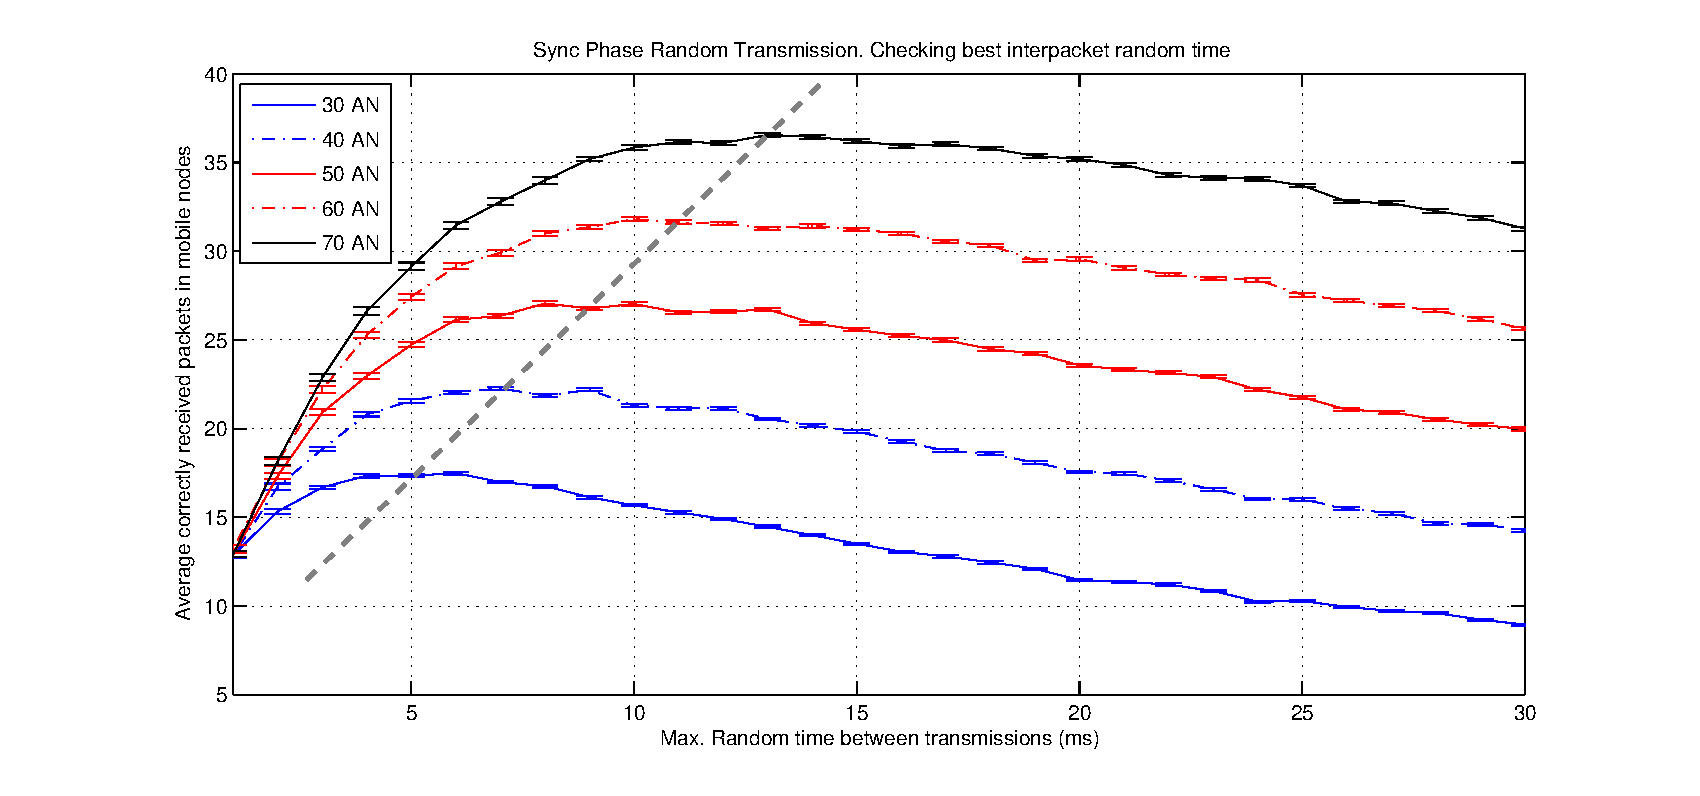
\includegraphics[width=1\textwidth]{randomTimeCheckingTheBestInterpacketRandomTime.eps}
 \end{center}
 \caption{Checking the best time between random transmissions}
 \label{fig:randomTimeCheckingTheBestInterpacketRandomTime}
\end{figure}

In this figure, it can be seen how when the time between transmissions is small, the number of delivered packets is also small. This is due to the 
collisions. When the time between transmissions grows, so does the correctly received packets until it reaches a maximum where it goes down again.
The ground for this is that the bigger the time between transmissions is, the less the number of packets that fit in the fixed Sync Phase time. When in 
Figure \ref{fig:receivedPacketsAndLastPacketArrival} there was no time limit, it could be seen how the received packets number did only grow.

From Figure \ref{fig:randomTimeCheckingTheBestInterpacketRandomTime}, it can also be seen that the more \acp{AN} there are, the more received packets and
the later the maximum comes. This maximum comes later because as the number of \acp{AN} is bigger, there are also more collisions, being its effect in the 
number of delivered packets bigger compared with the time between transmissions. And as the number of slots is bigger (hence the Sync Phase time), the 
time between transmissions influence will come later.

The gray discontinuous line was drawn following the maximum points for every curve. This line gives us the optimum waiting time between transmissions to 
be set for any number of \acp{AN}. Taking a smaller value generates more collisions and a bigger value makes the number of delivered packets smaller due
to the lack of time in the phase.

\subsubsection{Checking the best number of sent packets per \ac{AN}}

In this scenario, each \ac{AN} sends a maximum number of packets from 3 to 16 during the Sync Phase time defined by the slots. First, Computer calculates 
the number of slots and multiplies it by \textit{syncPacketsPerSyncPhase} (in this case 3) to obtain the Sync Phase time. This simulation will be done 
for different number of \acp{AN} (already told) where the previous optimal maximum random times between transmissions will be taken (see Table
\ref{tab:optimalTransmitTimes}). After repeating each case 100 times, \textbf{Figure \ref{fig:randomTimeCheckingTheBestNumberOfSentPacketsForAnchor}} 
is obtained.

\begin{table}
 \begin{center}
  \begin{tabular}{|l|c|}
   %\noalign{\vspace*{0.5cm}}
   \hline
   30 \acp{AN} & 5 ms \\
   \hline
   40 \acp{AN} & 7 ms \\
   \hline
   50 \acp{AN} & 9 ms \\
   \hline
   60 \acp{AN} & 11 ms \\
   \hline
   70 \acp{AN} & 13 ms \\
   \hline
  \end{tabular}
  \caption{Optimal maximal random times between \ac{AN} transmissions}
  \label{tab:optimalTransmitTimes}
 \end{center}
\end{table}

\begin{figure}[ht]
 \begin{center}
  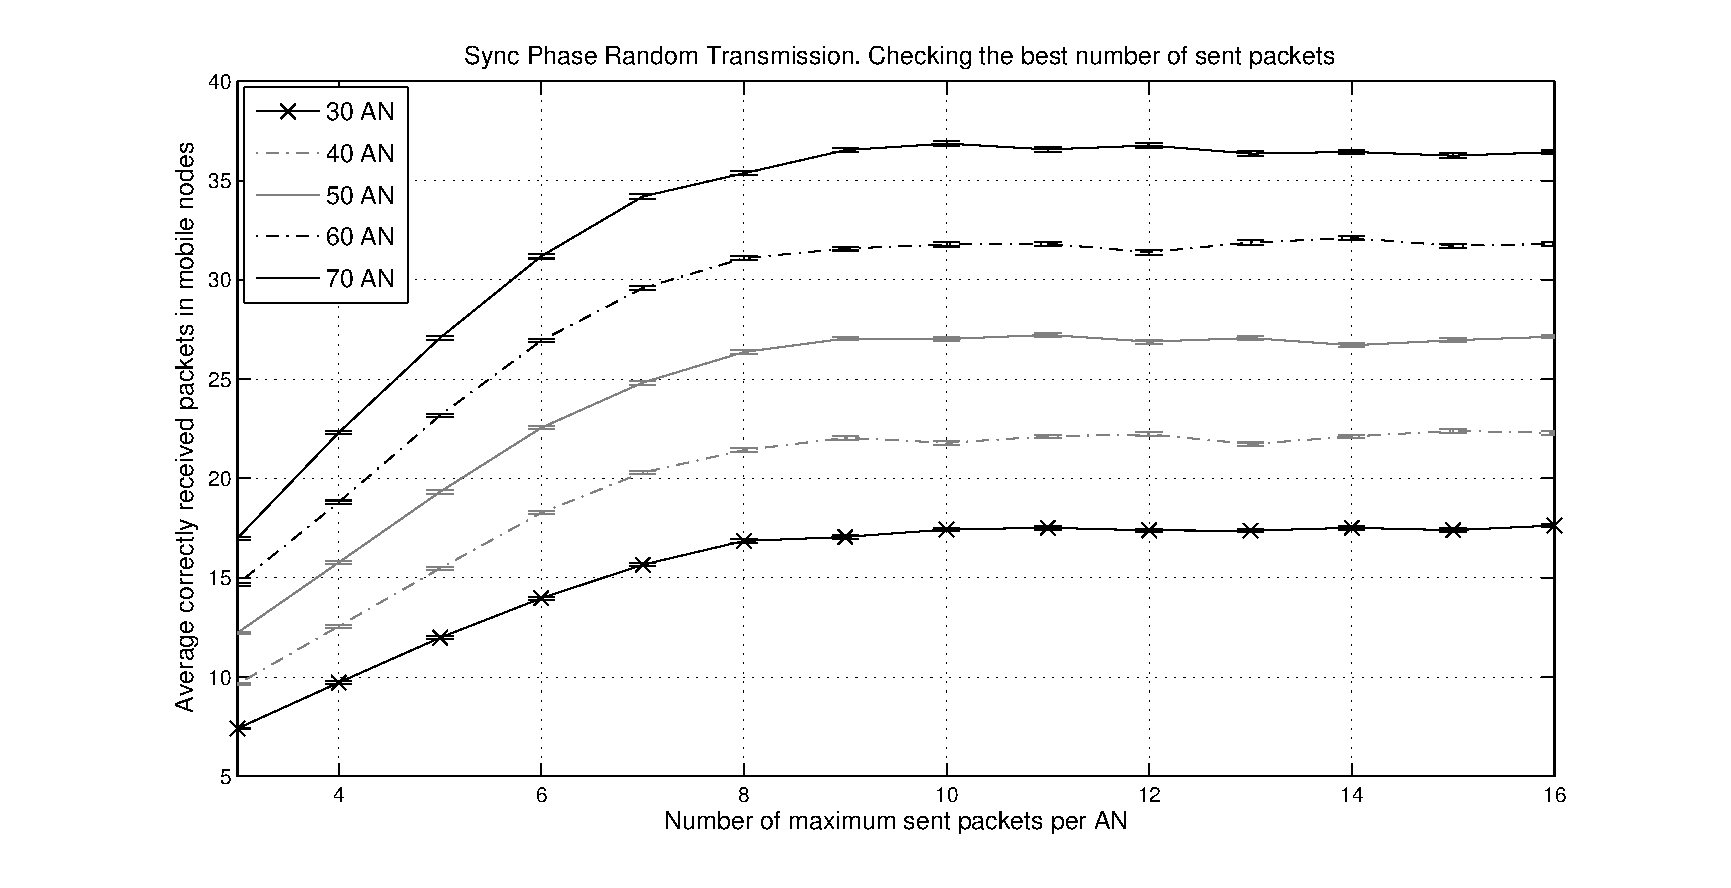
\includegraphics[width=1\textwidth]{randomTimeCheckingTheBestNumberOfSentPacketsForAnchor.eps}
 \end{center}
 \caption{Checking the best number of sent packets per \ac{AN}}
 \label{fig:randomTimeCheckingTheBestNumberOfSentPacketsForAnchor}
\end{figure}

It can be clearly seen in the figure, how the average number of received packets in the \acp{MN} increases until it reaches a maximum (approximately
with 10 sent packets). This is so because in the fixed Sync Phase time, there is no time for more packets to arrive. Ten is hence defined as the 
maximum number of packets to be sent. The reason to this limit is that when an \ac{AN} has already reached this maximum sent packets number per Sync Phase, 
it will stop sending more, leaving the channel more free for the rest of the \acp{AN} to transmit.

\subsubsection{Slotted vs. Best Random case comparison}

Both alternatives will be compared in a first approach checking the average number of packets received by the \acp{MN} in different situations. In 
all situations, cases with 30, 40, 50, 60 and 70 \acp{AN} will be studied. In the comparison there will be included the following situations: 
slotted case, best random transmissions case, worst random transmissions case ($T=1 ms$) and two random transmissions cases between worst and best cases
($T=3ms$ and $T=5ms$). Where T is the maximum random time between transmissions. In all cases the number of transmitted packet per \ac{AN} will be 10.

\begin{figure}[ht]
 \begin{center}
  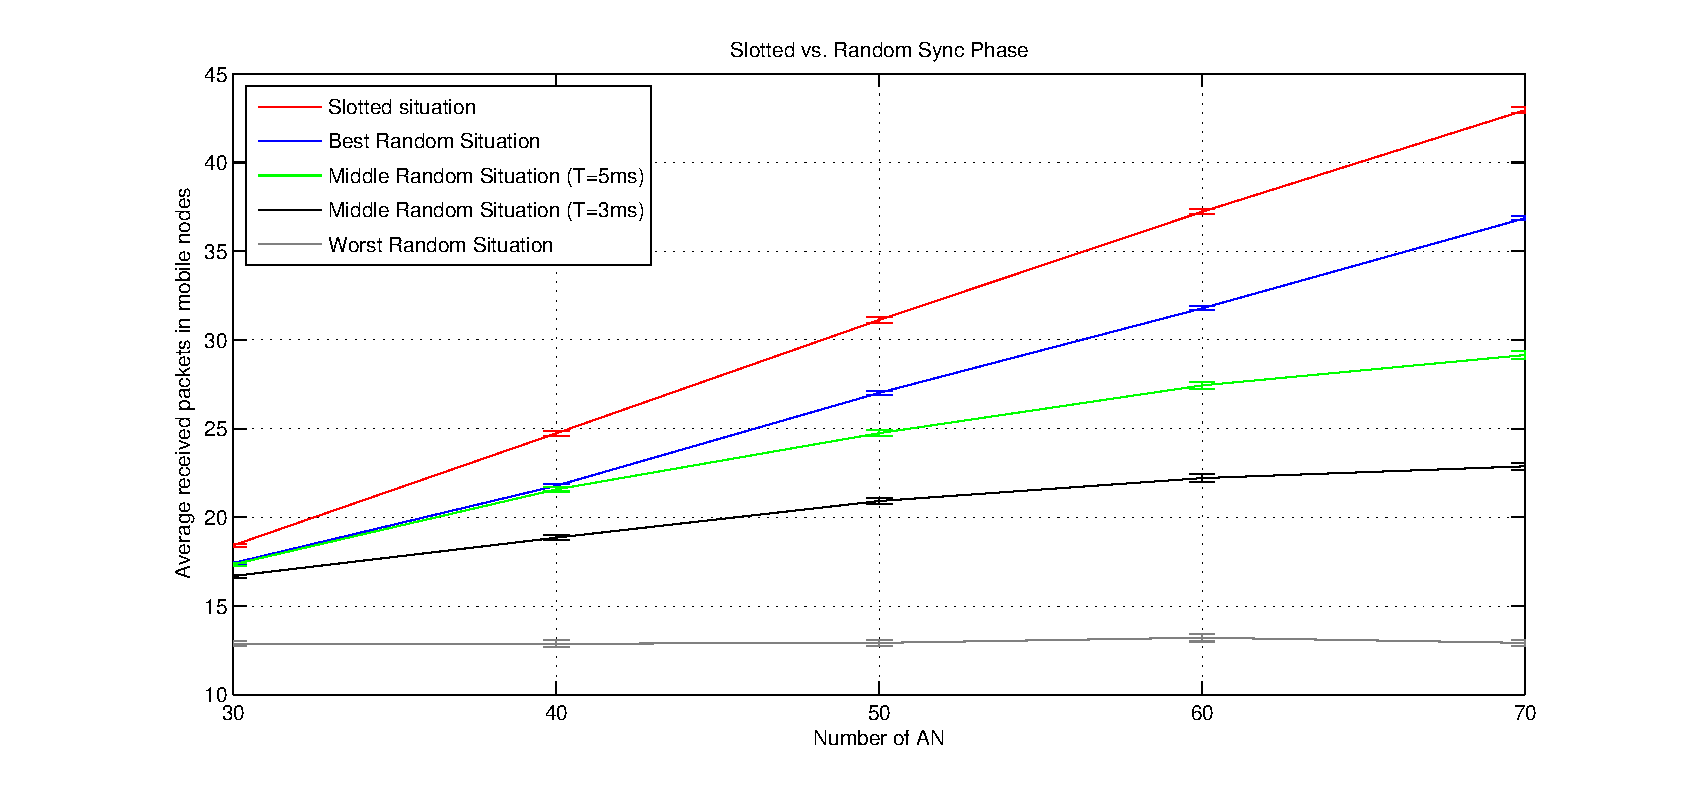
\includegraphics[width=1\textwidth]{slottedVsRandomAverageReceivedPackets.eps}
 \end{center}
 \caption{Slotted vs. Random cases comparison for number of received packets in \ac{MN}}
 \label{fig:slottedVsRandomAverageReceivedPackets}
\end{figure}

\textbf{Figure \ref{fig:slottedVsRandomAverageReceivedPackets}} shows how in all situations, in the slotted case \acp{MN} received more packets as in
any of the random cases. It can be also seen that this difference gets bigger when the number of \acp{AN} arises.

As a second comparison between the bestFrom all this, it can be obtained that slotted transmission is better than even the best case of random transmission. Slotted transmission will be hence
the one used during the Sync Phase in the complete protocol analysis. case for random transmissions and the slotted case, the number of first, second, third, fourth, \ldots, eighth
packets from an \ac{AN} received in the \ac{MN}, will be studied. Results can be seen in \textbf{Figure \ref{fig:numberOf1st2ndPacketsReceived}}.

\begin{figure}[ht]
 \begin{center}
  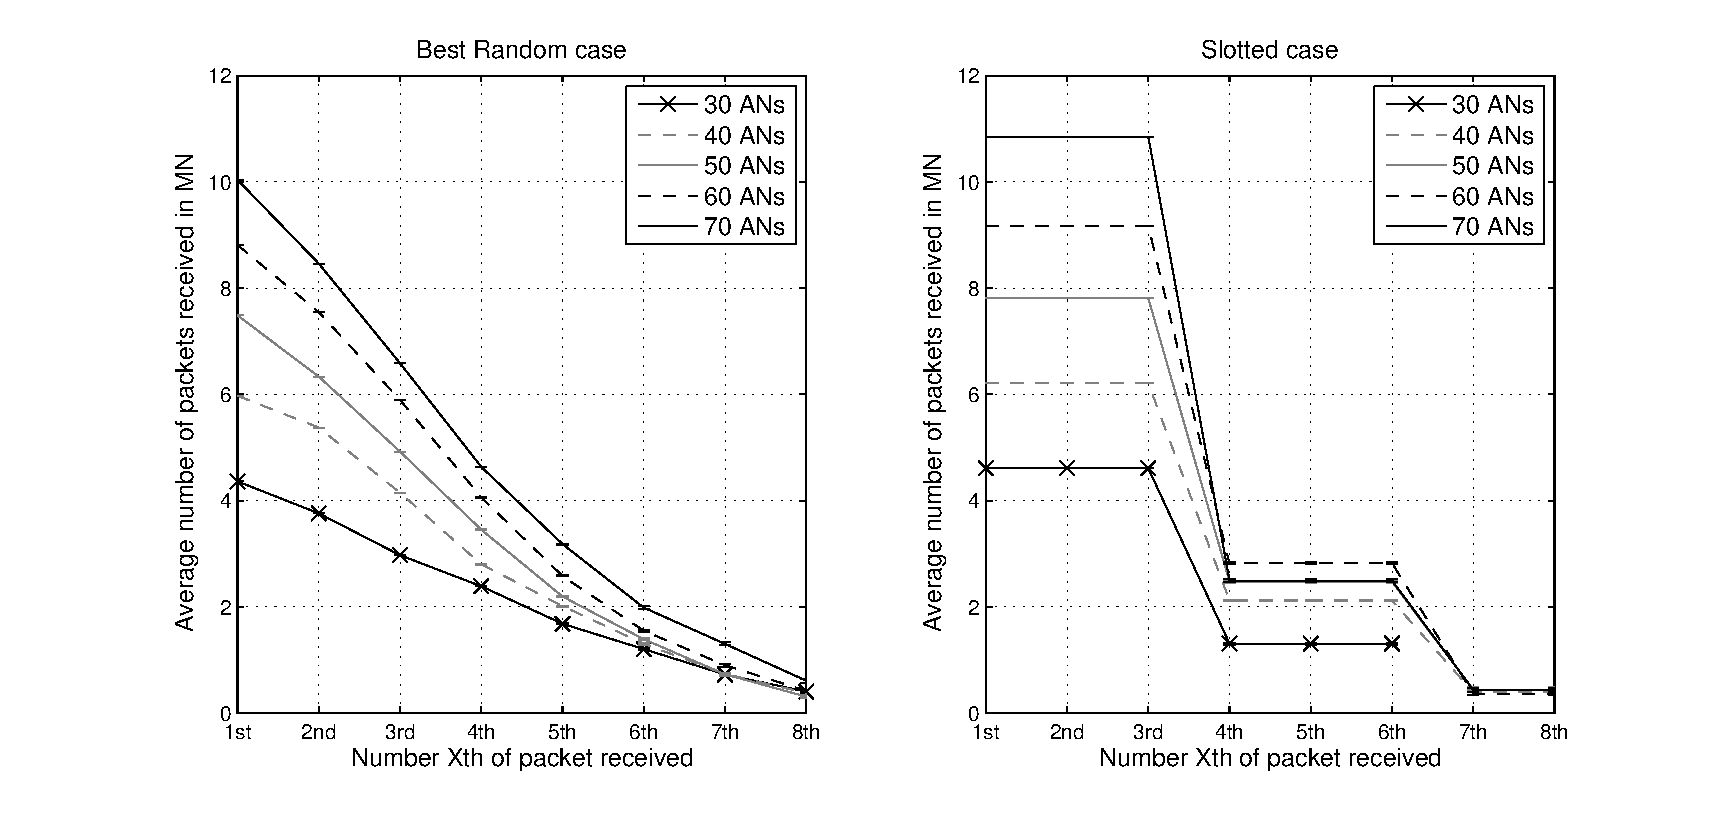
\includegraphics[width=1\textwidth]{numberOf1st2ndPacketsReceived.eps}
 \end{center}
 \caption{Number of $1^{st}$, $2^{nd}$, $3^{rd}$ \ldots, $8^{th}$ received packets in \acp{MN} from an \ac{AN}}
 \label{fig:numberOf1st2ndPacketsReceived}
\end{figure}

In both graphics can be appreciated how the more \acp{AN} there are, the more received packets in the \acp{MN}. It can be seen as well, how
for the slotted case, the number of received packets is bigger than for the random case (as it was already proved).

In the graphic on the left, it can be seen how the number of first packets received is bigger than the number of second packets. How the number of 
second packets received is bigger than the number of third packets, etc. And how this reduction occurs in a gradual way. Unlike this, in the graphic 
on the right, a stair-shaped behavior can be appreciated.

As \textit{syncPacketsPerSyncPhase} = 3, the Sync Phase will be divided into 3 identical sub phases. This means that all packets sent in one sub 
phase, will be sent in the other two. That is why the number of first, second and third packets is the same, as well as the number of fourth, fifth 
and sixth, and the number of seventh and eighth. Anytime a packet is sent more than \textit{syncPacketsPerSyncPhase} = 3 times, is due to slot re-using. 
That justifies why for example for the 30 \acp{AN} case, no seventh or eighth packets where sent, re-use here was not so big.

As a last comparison between slotted case and best random case, Packet arrival times in the \acp{MN} will be studied. Getting \textbf{Figure
\ref{fig:Lastarrivalpackettimes}} as the result to be commented. For a good understanding of this figure, X axis should be clarified. X axis has numbers
going from 1 to 11. Number from 1 to 8 represent the $1^{st}$, $2^{nd}$, $3^{rd}$ \ldots, $8^{th}$ last received packet in the \acp{MN}. Number 9 
represents the first packet arrived in the \acp{MN}. Number 10 represents the last packet arrived in the \acp{MN}. And number 11 represents the elapsed 
time between arrived packets in the \acp{MN}.

\begin{figure}[ht]
 \begin{center}
  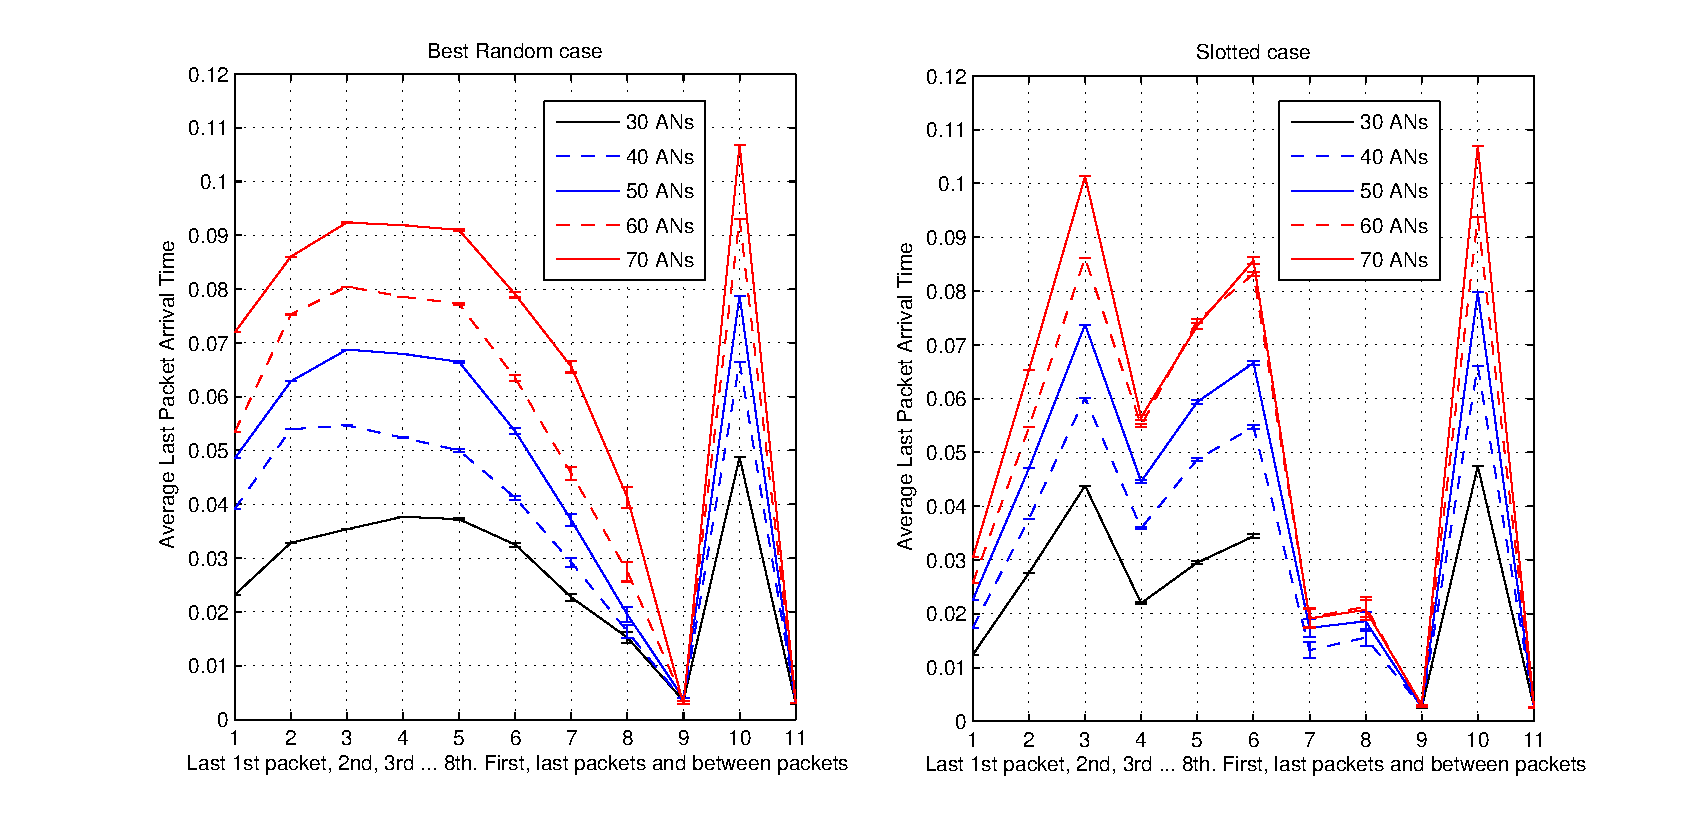
\includegraphics[width=1\textwidth]{Lastarrivalpackettimes.eps}
 \end{center}
 \caption{Different packet arrival times in the \acp{MN}}
 \label{fig:Lastarrivalpackettimes}
\end{figure}

Like for case in Figure \ref{fig:numberOf1st2ndPacketsReceived}, the more the \acp{AN} in the network, the bigger the time the \acp{MN} have to wait 
until they get the last packet.

Comparing both right and left graphics, it can be seen that the arrival times for the first ($X=9$) and last packet ($X=10$) and inter the arrival 
time ($X=11$), are very similar. This is so because this depends mainly on the duration of the Sync Phase more than on the way the packets are sent. 
Looking at the arrival time of the last packet ($X=10$), the length of the Sync Phase can be deduced. When looking to X axis values from 1 to 8, many
differences can be observed.

In the case of the graphic on the left (best random case), it can be seen that for small X values, the time of the last $X^{th}$ received packet 
grows with X. This is because all \acp{MN} receive many $1^{st}$, $2^{nd}$ or $3^{rd}$ packets, and the last of the $1^{st}$ packets should arrive 
before the last of the $2^{nd}$ and so on. But, why is it not like this until the last packet? The reason is that not many \acp{AN} are able to send
$5^{th}$, $6^{th}$, $7^{th}$ or $8^{th}$ packets being the $3^{rd}$ or $4^{th}$ the maximum packet they get to send. They are not able to send them
because the Sync Phase is limited in time, being than the $3^{rd}$ or $4^{th}$ packet sent at the end of the phase, raising thus the average arrival time
for this kind of packets.

In the slotted case graphic (on the right), the idea is the same as expressed before. The only difference is that, like in Figure 
\ref{fig:numberOf1st2ndPacketsReceived}, as \textit{syncPacketsPerSyncPhase} = 3, all behaviors are grouped. It can be seen that $1^{st}$, $2^{nd}$ and 
$3^{rd}$ last packets are together in one group. $4^{th}$, $5^{th}$ and $6^{th}$ last packets together in another group, and $7^{th}$ and $8^{th}$ in
another. Inside these groups the last $X^{th}$ arrived packet grows with X because, as the three sub phases in Sync Phase are the same, whenever a 
$4^{th}$ packet is delivered, this means that also a $5^{th}$ and $6^{th}$ packet will be.

Here it can also be observed, like in Figure \ref{fig:numberOf1st2ndPacketsReceived}, the re-usability of the slots. Seeing for example for the 
30 \acp{AN} case, that no seventh or eighth packets where sent because the re-use here was not so big.

\paragraph{Conclusion.} From all this results, it can be extracted that slotted transmission is better than even the best case of random transmission. 
Slotted transmission will be hence the one used during the Sync Phase in the complete protocol analysis.

\section{Framework simulation and analysis}

The aim of this section, is to analyze through different configurations the performance of the network for parameters like traffic or energy 
consumption among others.

The proposed scenario for this simulations is formed by 25 \acp{AN} distributed forming a grid, 60 \acp{MN} randomly and uniformly distributed in the
playground and a Computer. This scenario, with a size of 700 x 700 m, can be seen in Figure \ref{fig:finalscenario} . The \acp{AN} 
are distributed forming a grid to avoid the necessity to make a more complex routing protocol (explained in Chapter \ref{chap:protocolimplementation}: 
\nameref{chap:protocolimplementation}). Grid was also chosen because it was seen in many literature as a good standard way to study a network.

From the proposed grid, and with the help of the algorithm to assign slots (Sub-Section \ref{subsec:slottedsyncphase}: 
\nameref{subsec:slottedsyncphase}), it was obtained that 9 slots are the necessary ones to avoid Hidden Terminal Problem. This slots have the 
following distribution of \acp{AN}:

\begin{verbatim}
      Slot 0: 0, 3, 15, 18
      Slot 1: 1, 4, 16, 19
      Slot 2: 2, 17
      Slot 3: 5, 8, 20, 23
      Slot 4: 6, 9, 21, 24
      Slot 5: 7, 22
      Slot 6: 10, 13
      Slot 7: 11, 14
      Slot 8: 12
\end{verbatim}

\begin{figure}[ht]
 \begin{center}
  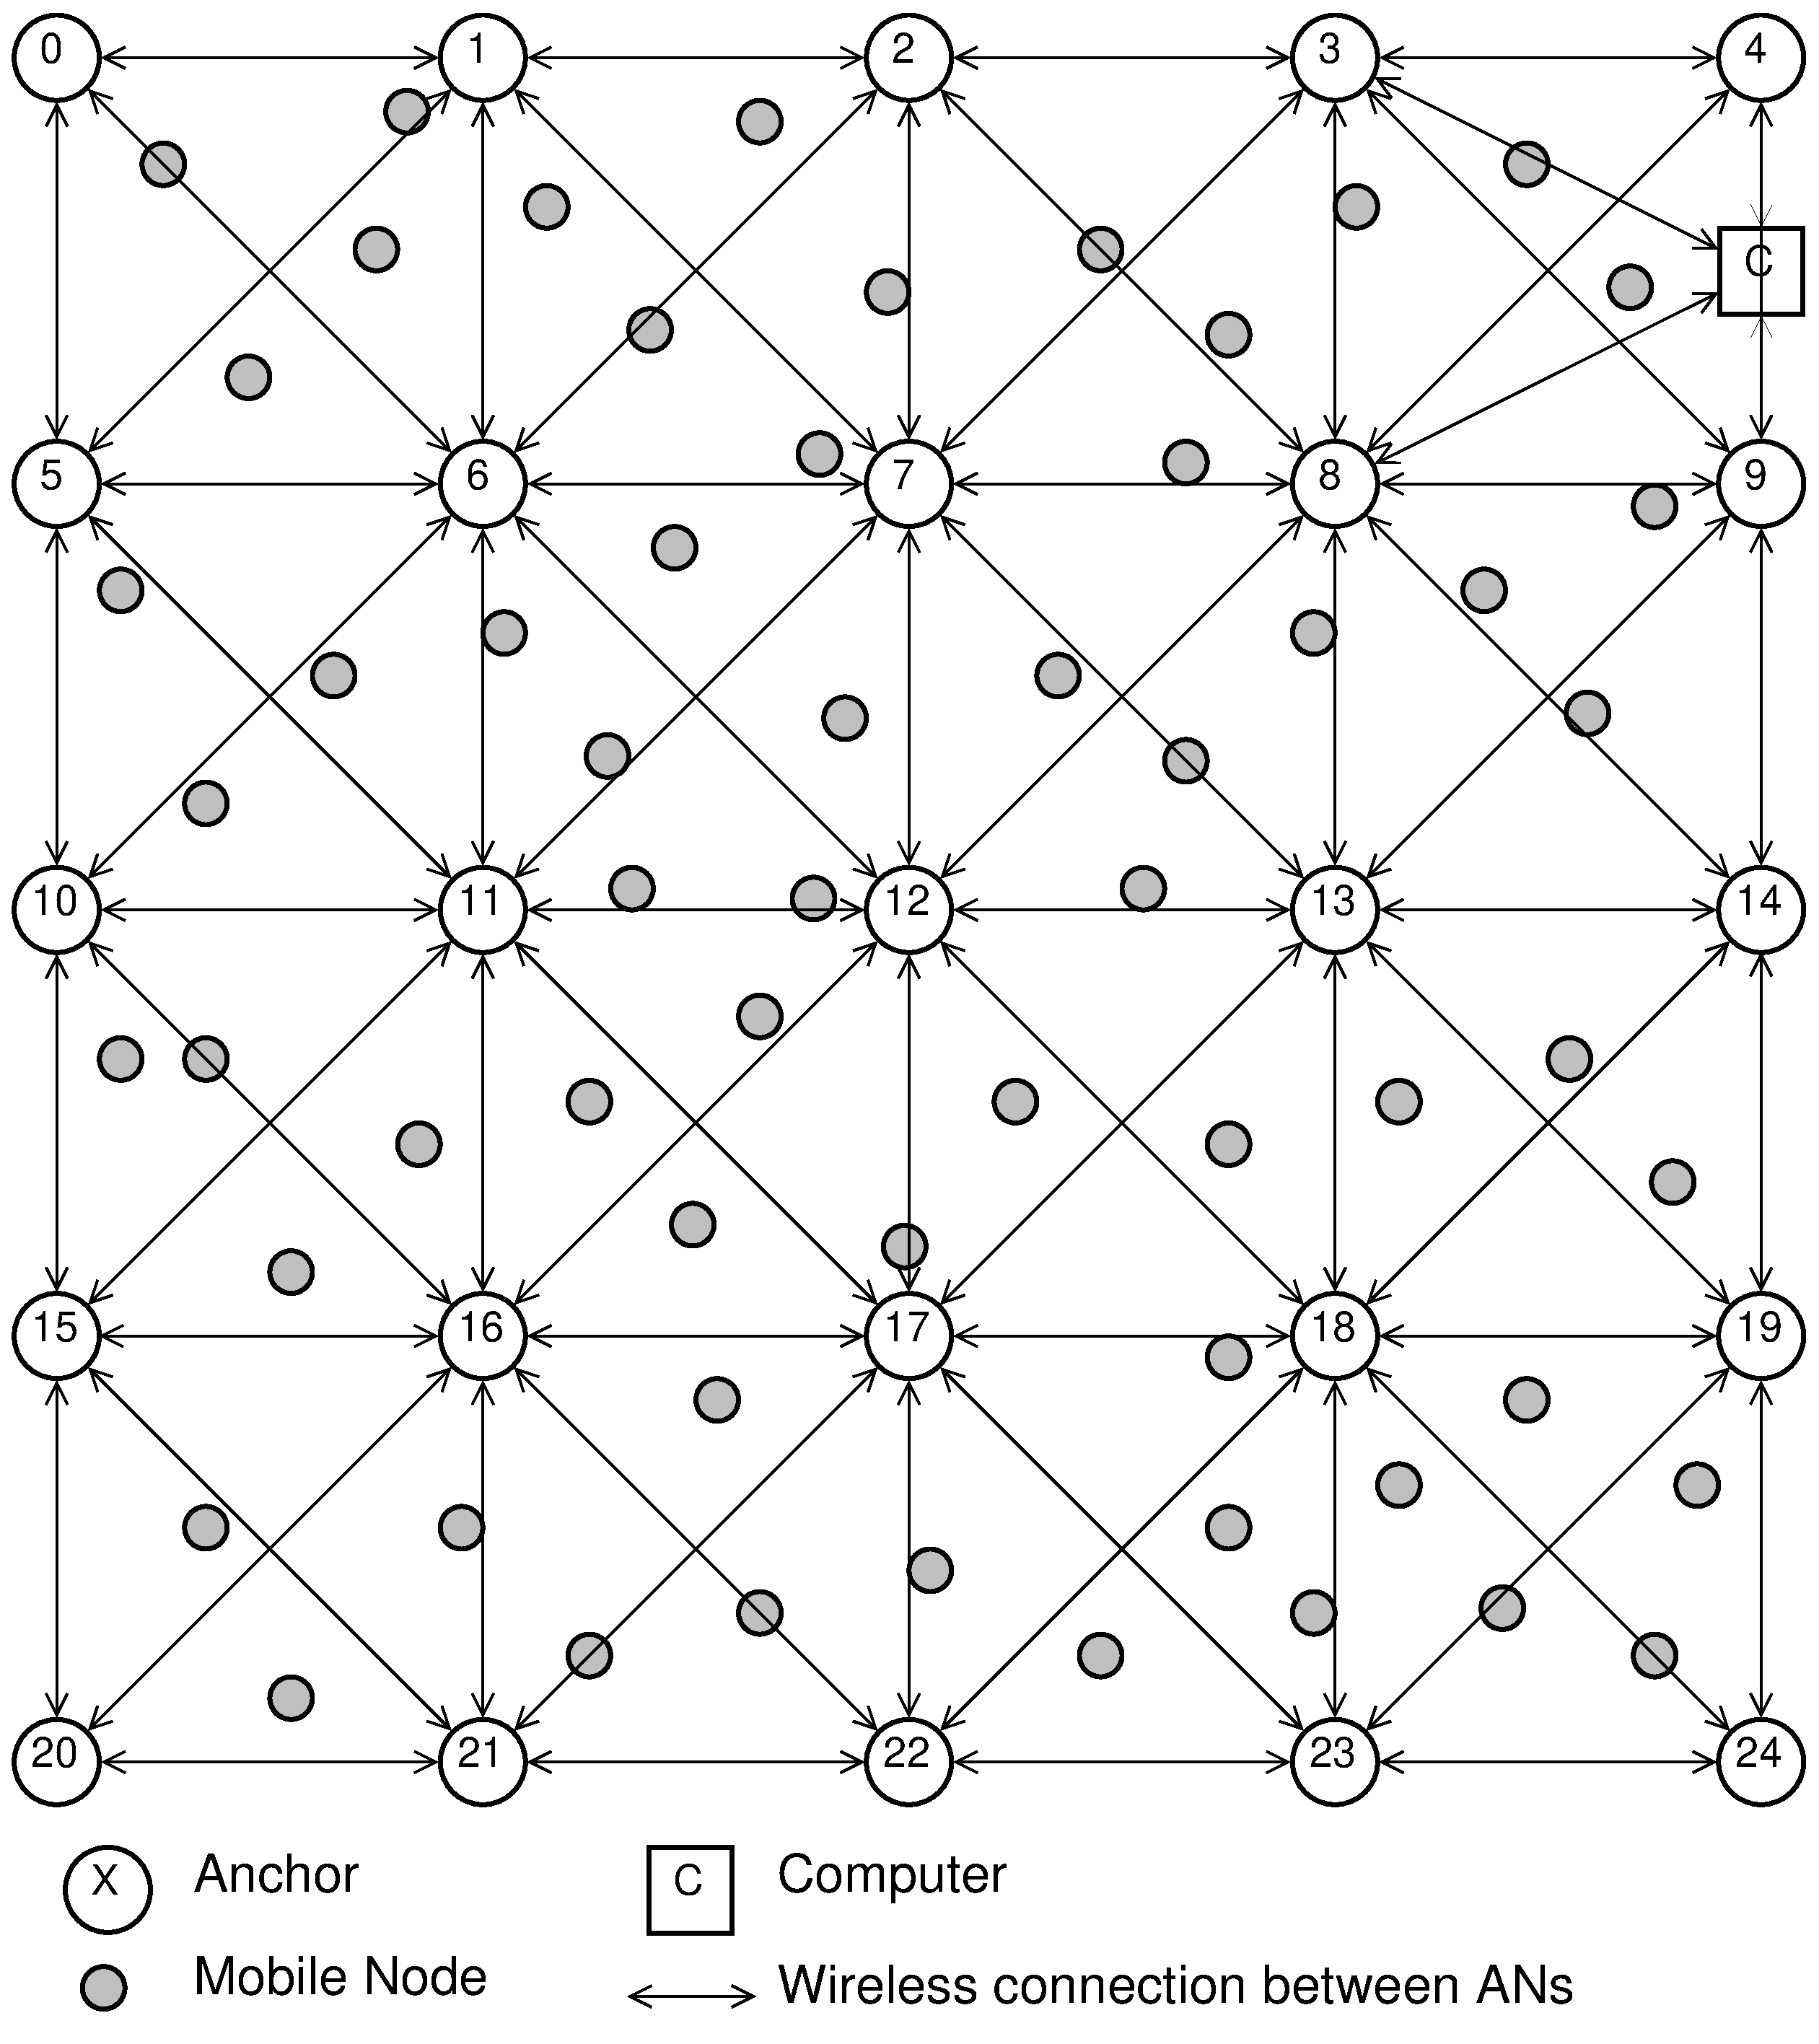
\includegraphics[width=0.5\textwidth]{finalscenario.eps}
 \end{center}
 \caption{Proposed scenario for High Configurable Protocol analysis}
 \label{fig:finalscenario}
\end{figure}

Considering that the period time is 1.5 s, the Com Sink Phases are 0.5 s each one and that there are $9\cdot3$ slots in each Sync Phase with 1.5 ms each one
of them. The following phases times are obtained:

\begin{verbatim}
    Sync Phases length:     0.0405 s
    Report Phase length:    0.2271 s
    VIP Phase length:       0.1514 s
    Com Sink Phases length: 0.5000 s
\end{verbatim}

To force different simulation situations and to be able to check the different \acp{MN} modes, ten configurations are going to be proposed. This 
configurations could be changed just modifying some parameters (explained in Section \ref{sec:ProtocolDescription}: \nameref{sec:ProtocolDescription}). 
Each one of this configurations is going to be simulated during 120 s (80 periods), and repeated 100 times to be able to compensate the dispersion 
generated by the generated random numbers. All graphics in this section will have on X axis this configurations.

The configurations are divided into two groups:

\begin{itemize}
 \item \textbf{Non distributed. }Groups the first five configurations, which are going to be the ones loading the network the most. All of this
configurations are going to have the following parameters in common:
\begin{verbatim}
 activePhases = 1
 inactivePhases = 0
 offsetPhases = 0
 offsetSyncPhases = 0
 reportPhases = 4 
 askFrequency = 2
 offsetReportPhases = 0
 NumberOfBroadcasts = 5
\end{verbatim}
As all the offsets are set to zero, all \acp{MN} will start their functionality at the beginning of the first period and all at the same
time. This is the reason why this group is called ``non distributed''. As it can be observed, inactive periods are set to 0, this way, all \acp{MN} will 
work every period, loading the network all the time. As \textit{reportPhases} = 4, \acp{MN} Mode 2 and 3 will report only 1 out 4 periods, loading even
more the network during this periods. Note also that the number of broadcast per \ac{MN} Mode 3 and 4 are five.

From this group, and attending to the number of \acp{MN} of each Mode (see Figure \ref{fig:ProtocolPhases}) this 5 configurations are proposed:
\begin{itemize}
 \item[-] \textbf{Config 1}: 15 \acp{MN} Mode 1, 15 \acp{MN} Mode 2, 15 \acp{MN} Mode 3 and 15 \acp{MN} Mode 4.
 \item[-] \textbf{Config 2}: 6 \acp{MN} Mode 1, 6 \acp{MN} Mode 2, 15 \acp{MN} Mode 3 and 33 \acp{MN} Mode 4.
 \item[-] \textbf{Config 3}: 6 \acp{MN} Mode 1, 6 \acp{MN} Mode 2, 33 \acp{MN} Mode 3 and 15 \acp{MN} Mode 4.
 \item[-] \textbf{Config 4}: 33 \acp{MN} Mode 1, 15 \acp{MN} Mode 2, 6 \acp{MN} Mode 3 and 6 \acp{MN} Mode 4.
 \item[-] \textbf{Config 5}: 15 \acp{MN} Mode 1, 33 \acp{MN} Mode 2, 6 \acp{MN} Mode 3 and 6 \acp{MN} Mode 4.
\end{itemize}
 \item \textbf{Distributed. }Groups the last five configurations, which are going to be the ones loading the network the less. All this
configurations are going to have the following parameters in common:
\begin{verbatim}
 activePhases = 2
 inactivePhases = 4
 offsetSyncPhases = 1
 reportPhases = 12
 askFrequency = 2
 NumberOfBroadcasts = 3
\end{verbatim}
This time, it can be seen that both \textit{offsetPhases} and \textit{offsetReportPhases} are not common parameters, this is because they are going to be
used to distribute all the \acp{MN} in the time in a way that $1/3$ of the \acp{MN} will start in period 0, another $1/3$ will start in period 2 and the 
rest $1/3$ will start in period 4. As \textit{activePhases} + \textit{inactivePhases} = 6, \acp{MN} will be perfectly distributed to load the network as 
low as possible. Due to the different kinds of \acp{MN}, the distribution in time will be done equally for every kind of \ac{MN}.

As \textit{reportPhases} = 12, \acp{MN} Mode 2 and 3 will report only 1 out 12 periods, that means they will almost not load the network. Note also that 
the number of broadcast per \ac{MN} Mode 3 and 4 is three instead of five.

From this group, and attending to the number of \acp{MN} of each Mode (see Figure \ref{fig:ProtocolPhases}) this 5 configurations are proposed:
\begin{itemize}
 \item[-] \textbf{Config 6}: 15 \acp{MN} Mode 1, 15 \acp{MN} Mode 2, 15 \acp{MN} Mode 3 and 15 \acp{MN} Mode 4.
 \item[-] \textbf{Config 7}: 6 \acp{MN} Mode 1, 6 \acp{MN} Mode 2, 15 \acp{MN} Mode 3 and 33 \acp{MN} Mode 4.
 \item[-] \textbf{Config 8}: 6 \acp{MN} Mode 1, 6 \acp{MN} Mode 2, 33 \acp{MN} Mode 3 and 15 \acp{MN} Mode 4.
 \item[-] \textbf{Config 9}: 33 \acp{MN} Mode 1, 15 \acp{MN} Mode 2, 6 \acp{MN} Mode 3 and 6 \acp{MN} Mode 4.
 \item[-] \textbf{Config 10}: 15 \acp{MN} Mode 1, 33 \acp{MN} Mode 2, 6 \acp{MN} Mode 3 and 6 \acp{MN} Mode 4.
\end{itemize}
Each of this configurations divide the number of \acp{MN} from each mode by 3, assigning the first third \textit{offsetPhases} = 0 and 
\textit{offsetReportPhases} = 2, the second third \textit{offsetPhases} = 2 and \textit{offsetReportPhases} = 4 and the third third
\textit{offsetPhases} = 4 and \textit{offsetReportPhases} = 6. This way all nodes will be equally distributed. That is why this group is called
``Distributed''. 
\end{itemize}








Tiempos simulacion


\clearpage{\pagestyle{empty}\cleardoublepage}
\chapter{Conclusions and future work}
\label{chap:conclusionsandfuture}

\section{Summary and Conclusions}

In this work the design of a High Configurable Protocol based on 802.15.4 standard is proposed. This protocol appears as a combination of two
previous proposals: \ac{LPL} and \ac{OLP}. Unlike this two proposals, this protocol allows \acp{MN} to operate in different modes according to 
their necessities and the situation of the network. Four operation modes are proposed. Mode 1 allows \acp{AN} or the Computer to estimate the 
\ac{MN}'s position using the reports sent by the \acp{MN}. This reports contain \ac{RSSI} measurements. This mode is equivalent to \ac{OLP}
approach. \acp{MN} in Mode 2 estimate their position their selves using low-complexity algorithms, avoiding the overload of the network. This 
position is estimated thanks to the captured \ac{RSSI} values. Mode 3 is used within \acp{MN} with a critical battery status. To make them 
consume as low as possible, this \acp{MN} do not listen to the channel but send their own broadcast packets to be detected by the \acp{AN}. 
This mode is equivalent to \ac{LPL}. And finally, an operational Mode 4 used by the \acp{MN} which need a high position accuracy. This is 
done combining the functionality in Modes 1 and 3.

The protocol's functionality is divided into periods which will be repeated periodically. Each period is divided into seven phases. During 
the first, fourth and sixth phases (Sync Phases) all nodes in the network are synchronized thanks to broadcast packets sent by the \acp{AN}. 
This broadcast packets are also used to provide to the \acp{MN} with \ac{RSSI} samples. The synchronization phase is divided into three parts 
to avoid correlation in \ac{RSSI} values between consecutive broadcast packets. During the second phase (Report Phase), all \acp{MN} send their
reports in case they have to. \acp{MN} configured in Mode 4 send also their broadcast packets. The third phase (\ac{VIP} Phase) is reserved for the \acp{MN} in Mode
3. During this phase they do not need to compete, with \acp{MN} in other modes, for the channel, to be able to send all their broadcast packets. 
The fifth and seventh phases are reserved for communication among \acp{AN} and the Computer.

This new protocol allows, changing the \ac{MN}'s configuration, to distribute the working periods of each \ac{MN} in time. This way the network
load will be distributed avoiding periods highly loaded compared with the others.

In the results, it is proved that \acp{MN} in Mode 3 consume much less energy than the \acp{MN} operating in other modes and, how,
this is independent of the simulated configuration. This shows how listening to broadcasted packets instead of transmitting them arises
the energy consumption. When the number of \acp{MN} in Modes 3 and 4 grows, it is seen, how, the energy consumption 
for this \acp{MN} also grows and, the performance of the ComSink Phases decreases. Hence, it is proved that \ac{LPL} configuration is not enough
for all situations, specially when the number of \acp{MN} is big. On the other hand, if all \acp{MN} were configured in Modes 1 and 2, the accuracy
and the energy consumption would be affected, revealing that \ac{OLP} configuration is not enough either. It is proved then, the necessity of
a High Configurable Protocol.

From the results can also be extracted that, independently of the configuration, the ComSink Phases are not enough to put up with all generated 
traffic. It becomes essential then to make these phases' duration longer, to reduce the overall traffic in the network by configuring most of 
the \acp{MN} in Modes 1 and 2 or to have a good distribution in time to avoid traffic concentration.

In this work two different approaches for Sync Phase were also studied. In the first approach the \acp{AN} transmit their broadcast packets randomly
in time. The best random transmission case, due to maximum random time between deliveries, is searched. In the second approach the \acp{AN} transmit
their broadcast packets distributed into time slots previously calculated by the Computer. From the results can be extracted that slotted 
transmission performance is better than even the best case of random transmission. Slotted transmission was, therefore, the one used during 
the Sync Phase in the complete protocol analysis. An automatic algorithm to calculate the slot distribution is also presented in this work.


\section{Future Work}

This work presents a stable and functional framework for a High Configurable Protocol based on 802.15.4 standard. However, all possible aspects
for a full protocol are not still contemplated. The following aspects could be still improved or developed:

\begin{itemize}
  \item \textbf{Change \ac{MN}'s configuration}. It was repeatedly said that \acp{MN} must adapt to network conditions and their own necessities. 
  The need of a \ac{MN}'s configuration change during the simulation depending on this aspects is still not contemplated in this work. The
  \acp{MN} are just configured at the beginning of the simulation.

  \item \textbf{Mobile \acp{MN}}. All this study was done for the case where all \acp{MN} stay in their original places. A study when the 
  \acp{MN} move around the playground would be also interesting.

  \item \textbf{Optimal configuration}. In this work a couple of configurations were tested to extract the first conclusions about
  this protocol. When using this protocol in a real situation, a deeper study of the configurations must be done. This way an optimal configuration
  could be used in each network situation.

  \item \textbf{Real network comparison}. Whenever this protocol is build in real devices, a deep comparison between simulation and real case should
  be done, to test the simulation validity.

  \item \textbf{Network division}. When network is too big, a division of the network into different areas could be beneficial, to avoid the high
  traffic during the ComSink Phases.

  \item \textbf{Broadcast \acp{AN}}. Another interesting case to be studied is an \acp{AN} division into two groups. One group would be the 
  \acp{AN} saw during this work, but, without the broadcasting function. A second group would be formed by \acp{AN} with a high power ability 
  which will transmit only the broadcast packets at a high power. This \acp{AN} will be able to reach all the network, synchronizing it 
  easily and in less time. This way idle time in \acp{MN} would be reduced and, for big networks, the synchronization problems due to long paths 
  and, the high routing traffic, would be avoided.

  \item \textbf{Reuse erased packets}. In this work packets are erased under many circumstances. In a future work these packets could be recovered
  or reused somehow not to lose them.

  \item \textbf{Full Network Layer}. To reduce the complexity of this project, the network layer routing was fixed, simulating always with the same
  \ac{AN}'s distribution. In a future, the Network Layer should calculate the routing automatically depending on the \ac{AN}'s position.

  \item \textbf{Aggregation and Segmentation}. In this work, \acp{AN} send a report for each \ac{MN}'s communication. To reduce traffic during
  ComSink Phases, it could be positive aggregating communications from different \acp{MN} in just one report. For this, aggregation must be added 
  to the protocol. When aggregated packets become too big, they must be segmented into smaller packets. This two capabilities should be implemented
  in the Transport Layer which does nothing in this work.

  \item \textbf{Real information in packets}. As this work's aim is to develop a working framework to test the protocol. All packet's 
  information is not real, being the only important aspect of a packet, its size. For a more realistic behavior, packets should carry 
  real information and, its handling should depend on this information.

  \item \textbf{ComSink Phases study}. It was seen how this phases are the most critical in this protocol. A deeper study of this phases
  should be done. An analysis of the advantages and disadvantages of, joining them in one bigger ComSink, taking out the up-links and down-links 
  restriction or further studies, should be done.

  \item \textbf{Queue priorities}. This work assumes all message's priority the same, putting them in a \ac{FIFO} queue. But as all messages have
  not the same importance, a priority queue should be developed. The messages should also have a life time, as some messages would be occupying 
  the queues even when they are not important anymore.

\end{itemize}

\clearpage{\pagestyle{empty}\cleardoublepage}

\appendix

\cleardoublepage
\pagestyle{fancy}
\chapter{Source code first contact}
\label{chap:installation}

This appendix will give a basic explanation about the control version tool used during this work. It will also introduce how to deal with 
the contents in the \ac{DVD} for the first time. All the steps will be explained for the Linux case, more precisely for Ubuntu 10.04.

\section{Git Introduction}

All backups during this work were done with a version control program called GIT \cite{git}. It is recommended to read a good tutorial to get
to work with it \cite{manualgit}.

In GIT, there are two important files:

\begin{itemize}
  \item \textbf{.gitconfig} - This file is located on the home directory and its content defines the author, some shortcuts and other configurations.
  The file used in this work is like follows.
  \begin{verbatim}
[user]
  name = Jorge Perez
  email = jorgeperezhidalgo@gmail.com
[alias]
  co = checkout
  ci = commit
  st = status
  br = branch
  hist = log --pretty=format:\"%h %ad | %s%d [%an]\" --graph --date=short
  type = cat-file -t
  dump = cat-file -p
[merge]
  tool = vimdiff
  \end{verbatim}

  Before continuing reading, it is recommended to create also this file changing the name and email because from now on, all aliases are going to
  be used. A copy of this file can be found in the root directory of the \ac{DVD}.

  \item \textbf{.gitignore} - Not all files in the working directory are important to be saved in a backup, for example, compiled files, documents, 
  etc. are not important. In this file it is defined which files are going to be saved and which not. This file should be placed in the root working
  directory, in this case the \verb|MiXiM| directory. To get a detailed description of this file's format, please refer to \cite{manualgit}. A copy of 
  this file can be found in \verb|MiXiM| directory in the \ac{DVD}.
  
\end{itemize}


\section{First contact}

First thing to do is installing \ac{OMNeT++} 4.0 \cite{OMNeT}. It can be easily done following \cite{installationomnet}. To follow this guide, 
\ac{OMNeT++} 4.0 must be installed in the home directory.

After that, copy the \verb|MiXiM| directory from the \ac{DVD} to the \verb|~/omnetpp-4.1/samples/| directory and, open the \ac{OMNeT++} 4.0.

Once the program is opened, the MiXiM project must be imported. For that click on ``File'' and than ``Import''. In the new window select 
``Existing Projects into Workspace'' from the ``General'' menu.

Assure ``Select root directory'' is selected and browse the 
\verb|~/omnetpp-4.1/samples/MiXiM/| directory. Than click on ``Finish''. Than the new project must be compiled, that is done by pressing ``Ctrl. + B''.
To run the last version, first a configuration should be done, this can be done following \cite{manualomnet}.

To see a history of all the versions in the project, from a terminal window and inside \verb|~/omnetpp-4.1/samples/MiXiM/| directory, \verb|git hist --all|
must be execute, obtaining the following output.

\footnotesize
\begin{verbatim}
~/omnetpp-4.1/samples/MiXiM$ git hist --all
* e821eb8 2011-08-19 | Correcting document (HEAD, origin/master, origin/HEAD, master) [Jorg...
* fe8ce36 2011-08-17 | Chapters 1 to 5 ready. Chapters 1 to 3 reviewed with Caro [Jorge Perez]
* 0f6887c 2011-08-15 | Correcting chapters and finishing chapter 4 in document [Jorge Perez]
* af6a4d3 2011-08-11 | Completing document chapter 4 [Jorge Perez]
* 682758c 2011-08-10 | Revised all graphics and finished chapter 5 in document [Jorge Perez]
* d12d184 2011-08-08 | Started document chapter 5, done some new graphics [Jorge Perez]
* 907b88b 2011-08-08 | Added another slots number graphic [Jorge Perez]
* 8baff00 2011-08-07 | Starting document chapter 4 [Jorge Perez]
* f41f67d 2011-08-06 | Ended document chapter 3 [Jorge Perez]
* 63d3c92 2011-08-05 | Continuing document chapter 3 [Jorge Perez]
* e163b2f 2011-08-04 | First contact with final simulation [Jorge Perez]
* c37d1b1 2011-08-02 | Document Chapter 3 start [Jorge Perez]
* be45e73 2011-07-27 | Added different packet sizes and different network configurations [J...
* a56a4b5 2011-07-26 | Document Chapter 1 and 2 ready [Jorge Perez]
* db46eca 2011-07-23 | LaTeX document structure done [Jorge Perez]
* c201800 2011-07-21 | Corrected error: going to Rx when a transmission ready, in App layer...
* 790553c 2011-07-13 | First steps writing the project with LaTeX [Jorge Perez]
* 8046976 2011-06-06 | Sleeping the Nodes and waking them up [Jorge Perez]
* aa8459d 2011-06-01 | Restructuring the configuration phases to reduce the number of event...
* 1cb3f90 2011-05-19 | Solving some problems when having a Broadcast MN type [Jorge Perez]
* 796160b 2011-05-04 | Mobile Nodes Types and Behaviour (frequencies, active and inactive f...
* 3bf9dfb 2011-05-02 | Slotted & Random Modes comparison graphics saved and commented [Jorg...
* 7cf1f71 2011-04-26 | RSSI info forwarded to App layer to start with phase organization [J...
* e912ccb 2011-04-18 | Corrected some general misstakes and ROUTING WORKING [Jorge Perez]
* 467d069 2011-04-13 | Added automatic grid location for Anchors [Jorge Perez]
* cfd79e0 2011-04-12 | Comparison between sloted phase 1 and random phase 1 [Jorge Perez]
* 88d0229 2011-04-11 | Check the total number of slots in sync phase when changing the dens...
* 2cf324f 2011-04-11 | Added Net and Trans Layer for Nodes and Computer [Jorge Perez]
* 6fa2e53 2011-04-07 | Added Net and Trans Layer to Anchor and deleted not useful files fro...
* f2d8e00 2011-04-04 | Added computer entity and anchor density distribution in map [Jorge ...
* f678d11 2011-02-22 | Added random transmision in phase 1 with results in Matlab [Jorge Pe...
* 04db6aa 2011-02-03 | Anchors transmit in every slot and model adapted to all phases [Jorg...
* 54dd74f 2011-01-25 | Added the slot division and assigned one or more slots to every Anch...
* 871f78d 2011-01-20 | Place anchor and mobile nodes randomly in the map with minimum separ...
* d713063 2011-01-20 | First Commit [Jorge Perez]
\end{verbatim}
\normalsize

It can be observed how each version has a reference number, the modification date, a description and the name of the person who modified
it. The ``HEAD'' word indicates which version is the current one and ``origin'' is the last saved version.

To change to an specific version execute, for example, \verb|git reset --hard 8046976|. And to go back to last version \verb|git reset --hard origin|.
This way all tracked files are changed to the desired version. To start another version from a specific point read about ``branches'' in
\cite{manualgit}. Remember to recompile the code in \ac{OMNeT++} by pressing ``Ctrl. + B'' each time the version is changed, as compiled
files are not saved in the backup.

MiXiM has many examples apart from the one studied by this work. This example is contained in directory \verb|~/omnetpp-4.1/samples/MiXiM/examples/ieee802154Narrow/|.

In the folder \verb|Resultados| in \verb|~/omnetpp-4.1/samples/MiXiM/examples/ieee802154Narrow/| directory are all the Matlab files necessary to plot
all the results contained in the work.

In the folder \verb|Proyecto| in \verb|~/omnetpp-4.1/samples/MiXiM/examples/ieee802154Narrow/| directory can be found this work document made in \LaTeX{}.

The \ac{DVD} folders \verb|Documents| and \verb|Programs| contain the documents and programs used during the development of this work.


\clearpage{\pagestyle{empty}\cleardoublepage}
\pagestyle{plain}
\chapter{Acronyms}
\label{chap:acronyms}
\begin{acronym}[OMNeT++]
%\setlength{\itemsep}{-\parsep}
  \acro{ACK}{Acknowledgement}
  \acro{AN}{Anchor Node}
  \acro{BE}{BackOff Exponent}
  \acro{CAF}{Channel Access Failure}
  \acro{CCA}{Clear Channel Assessment}
  \acro{CD}{Compact Disk}
  \acro{CRC}{Cyclic Redundancy Code}
  \acro{CSMA/CA}{Carrier Sense Multiple Access with Collision Avoidance}
  \acro{DVD}{Digital Versatile Disc}
  \acro{ED}{Energy Detection}
  \acro{FCS}{Frame Control Sequence}
  \acro{FFD}{Full Function Device}
  \acro{FIFO}{First In First Out}
  \acro{FSM}{Finite State Machine}
  \acro{GTS}{Guaranteed Time Slot}
  \acro{IEEE}{Institute of Electrical and Electronics Engineers}
  \acro{KO}{Knocked Out}
  \acro{LIFS}{Long Inter Frame Spacing}
  \acro{LPL}{Low Power Localization}
  \acro{LQI}{Link Quality Indication}
  \acro{LR-WPAN}{Low Rate WPAN}
  \acro{MAC}{Media Access Control}
  \acro{MATLAB}{Matrix Laboratory}
  \acro{MFR}{MAC Footer}
  \acro{MHR}{MAC Header}
  \acro{MiXiM}{Mixed Simulator}
  \acro{MN}{Mobile Node}
  \acro{MP3}{Moving Picture Experts Group Audio Layer III}
  \acro{NB}{Number of Backoffs}
  \acro{NED}{Network Description}
  \acro{NIC}{Network Interface Card}
  \acro{OLP}{Optimized Listening Period}
  \acro{OMNeT++}{Objective Modular Network Testbed}
  \acro{O-QPSK}{Offset quadrature phase-shift keying}
  \acro{PAN}{Personal Area Networks}
  \acro{PDA}{Personal Data Assistant}
  \acro{PHY}{Physical Layer}
  \acro{RFD}{Reduced Function Device}
  \acro{RSSI}{Received Signal Strength Indicator}
  \acro{Rx}{Reception}
  \acro{SIFS}{Short Inter Frame Spacing}
  \acro{Tx}{Transmission}
  \acro{uC}[$\mu$C]{MicroController}
  \acro{VIP}{Very Important Priority}
  \acro{WPAN}{Wireless Personal Area Networks}
  \acro{WSN}{Wireless Sensor Networks}
  \end{acronym}

\clearpage{\pagestyle{empty}\cleardoublepage}
\bibliographystyle{unsrt}
\bibliography{bib}
\pagestyle{plain}


% Pages with extra content of the document
%\appendix

\end{document}